%
% PhD Thesis
%
\documentclass[11pt,a4paper,twoside,openright]{book}

%
% Version: 0.0
%
% Semantic versioning (aka SemVer) [...] uses a sequence of three digits (Major.Minor.Patch) [...]
% Breaking changes are indicated by increasing the major number (high risk),
% new non-breaking features increment the minor number (medium risk) and
% all other non-breaking changes increment the patch number (lowest risk).

% 
% Specifications
%
% Ref: https://www.cambridgestudents.cam.ac.uk/your-course/examinations/graduate-exam-information/submitting-and-examination/phd-msc-mlitt/word#biology
%
% - The thesis for the PhD is not to exceed 60,000 words in length (80,000 by
%   special permission), exclusive of tables, footnotes, bibliography, and
%   appendices.
% - A4 portrait
% - Double-spaced or one-and-a-half spaced (one-and-a-half recommended by general Cambridge guidelines).
% - Single or double-sided printing (double-sided recommended by general Cambridge guidelines).

%
% Preamble
%
% \input{filename} imports the commands from filename.tex into the target file;
% it's equivalent to typing all the commands from filename.tex right into the
% current file where the \input line is.
%
% Preamble
%
% https://tex.stackexchange.com/questions/553/what-packages-do-people-load-by-default-in-latex

%
% Typesetting
%

% https://tex.stackexchange.com/questions/44694/fontenc-vs-inputenc
%
% Use modern font encoding
% fontenc is oriented to output, that is, what fonts to use for printing characters.
\usepackage[T1]{fontenc}
% inputenc allows the user to input accented characters directly from the keyboard
\usepackage[utf8]{inputenc}

% Correct hyphenation
% Specify patterns using e.g.  \hyphenation{hy-phen-a-tion MATLAB}
\usepackage[english]{babel}

% Typographic optimisation
% It doesn't work with latex, you have to use pdflatex instead.
\usepackage{microtype}

% Better Computer Modern font
\usepackage{lmodern}

% Extension package to amsmath
\usepackage{mathtools}
% Extended symbol collection
\usepackage{amssymb}
% For theorems
\usepackage{amsthm}

% Context-sensitive quotes, provides \enquote
%
% When using babel or polyglossia with biblatex, loading csquotes is recommended
% to ensure that quoted texts are typeset according to the rules of your main
% language.
\usepackage{csquotes}

%
% Document structure
%

% Automatically adds the bibliography and/or the index and/or the contents, etc.,
% to the Table of Contents listing.
\usepackage[nottoc]{tocbibind}

% Increase the value of tocdepth and secnumdepth. The tocdepth value determines
% to which level the sectioning commands are printed in the ToC (they are always
% included in the .toc file but ignored otherwise). The secnumdepth value
% determines up to what level the sectioning titles are numbered.
\setcounter{tocdepth}{3}
\setcounter{secnumdepth}{3}

% Extra control of appendices
% \usepackage[toc]{appendix}

%
% Figures and tables
%

\usepackage{graphicx}
\usepackage[font={footnotesize}]{caption}
\usepackage[font={footnotesize}]{subcaption}
% Changes the filename algorithm to check for known graphics extensions
\usepackage{grffile} 
% Using \usepackage{flafter} avoids figures floating before they were defined
\usepackage{flafter}

% Nicer tables
\usepackage{booktabs}

% Pretty-print code
\usepackage{listings}

% Define box for scaling tables
\usepackage{adjustbox}

%
% Formatting and appearance
%

% Format numbers using e.g. \numprint{2.742647826672E-01}
\usepackage{numprint}

% Format si units
\usepackage{siunitx}

% Define line spacing
% Setspace switches off double-spacing at places where even the most die-hard
% official would doubt its utility (footnotes, figure captions, and so on); it’s
% very difficult to do this consistently if you’re manipulating \baselinestretch
% yourself.
\usepackage{setspace}
\onehalfspacing

% 1 space after punctuation
\frenchspacing

% Extensive control of page headers and footers
\usepackage{fancyhdr}
\pagestyle{fancy}

% Allow modifications to enumerate lists
\usepackage{enumitem}

% Defines an outline environment, which allows outline-style indented lists with freely mixed levels up to four levels deep.
\usepackage{outlines}

%
% Navigation
%

% Clickable links
\usepackage{hyperref}
% Nice colors for clickable links
\usepackage{xcolor}
\usepackage{bookmark}
\hypersetup{
	colorlinks,
	linkcolor={red!50!black},
	citecolor={blue!70!black},
	urlcolor={blue!60!black}
}

%
% Misc
%
%
% TO-DO command and list
%
\usepackage{todonotes}
%
% Allow dummy text
%
\usepackage{lipsum}

%
% Bibliography
%
% https://tex.stackexchange.com/questions/25701/bibtex-vs-biber-and-biblatex-vs-natbib
%
% bibtex and biber are external programs that process bibliography information
% and act (roughly) as the interface between your .bib file and your LaTeX
% document.
% natbib and biblatex are LaTeX packages that format citations and
% bibliographies; natbib works only with bibtex, while biblatex (at the
% moment) works with both bibtex and biber.)

% https://leesjohn.wordpress.com/2013/04/22/a-latex-bibliography-style-i-like-nature-style-in-biblatex/
\usepackage[
	style=nature,
	maxcitenames=1,
	maxnames=6,
    giveninits=true,
	uniquename=init,
	sorting=none,
	url=false,
	doi=true,
	isbn=false,
	eprint=false,
	texencoding=utf8,
	bibencoding=utf8,
	autocite=superscript,
	backend=biber
]{biblatex}
% 
% NOTE: this is a path relative to main.tex
\addbibresource{backmatter/zotero_My-Library_phd_Better-BibLaTeX.bib}

%
% Abbreviations
%
% NOTE: there are certain packages that must be loaded before glossaries, if
% they are required: hyperref, babel, polyglossia, inputenc and fontenc.
\usepackage[
    abbreviations,
    % nohypertypes={abbreviations}
]{glossaries-extra}
%
% Set first use of abbreviation to appear expanded.
\setabbreviationstyle{long-short}
% use TeX to sort (slow)
\makenoidxglossaries
%
% Definitions
%
% \newabbreviation[⟨options⟩]{⟨label⟩}{⟨short⟩}{⟨long⟩}
\newabbreviation[longplural=genome-wide association studies]{GWAS}{GWAS}{genome-wide association study}
\newabbreviation[longplural=expression quantitative trait loci]{eQTL}{eQTL}{expression quantitative trait locus}
\newabbreviation[longplural=quantitative trait loci]{QTL}{QTL}{quantitative trait locus}
\newabbreviation[]{HIRD}{HIRD}{Human Immune Response Dynamics}
\newabbreviation[]{TRI}{TRI}{Titre Response Index}
\newabbreviation[]{RNAseq}{RNA-seq}{RNA-sequencing}
\newabbreviation[]{DE}{DE}{differential expression; differentially expressed}
\newabbreviation[]{DGE}{DGE}{differential gene expression}
\newabbreviation[]{HAI}{HAI}{haemagglutination inhibition}
\newabbreviation[]{MN}{MN}{microneutralisation}
\newabbreviation[]{PBMC}{PBMC}{peripheral blood mononuclear cell}
%


%
%
%
\begin{document}

\title{<title>}
\author{Benjamin Yu Hang Bai}
\date{<date>}

%
% Frontmatter
% Overall format based on: Mori, L. F. Writing a thesis with LaTeX.
%
\frontmatter

% \include{filename} essentially does a \clearpage before and after
% \input{filename}, [...] is primarily useful when you have a big project on a slow
% computer; changing one of the include targets won't force you to regenerate the
% outputs of all the rest. [...] but it also can't be nested, can't
% appear in the preamble, and forces page breaks around the included text.
%
% https://www.cambridgestudents.cam.ac.uk/your-course/examinations/graduate-exam-information/submitting-and-examination/phd-msc-mlitt/submit
% 1. A title page displaying:
%     the full title of the thesis,
%     your full name (as it appears on your passport),
%     your college,
%     the date of your submission (month and year)
%     and a declaration stating: "This thesis is submitted for the degree of Doctor of Philosophy/Master of Science/Master of Letters (as appropriate)."

% \maketitle

\begin{titlepage}
    \begin{center}
            
        \null
        \vspace{\stretch{13}}

        \Huge
        Genomic profiling of response to\\
        \textit{in~vivo} immune perturbations

        \vspace{1em}
            
        \Large
        Benjamin Yu Hang Bai

        \vspace{2em}
            
        
\includegraphics[width=0.3\textwidth]{frontmatter/figures/Churchill_College_Crest.pdf}

        \vspace{1em}
            
        Churchill College

        University of Cambridge

        Wellcome Sanger Institute

        \vspace{1em}

        November 2020

        \vspace{1em}

        \normalsize
        This thesis is submitted for the degree of Doctor of Philosophy

        \vspace{\stretch{21}}
        \null
            
    \end{center}
\end{titlepage}

%
% Dedication
%

% Set ratio of vertical space before and after dedication.
\null
\vspace{\stretch{1}}

\begin{flushright}
    % \textit{The more you know, the more you know you don't know.}
    % \url{https://www.poetsgraves.co.uk/Classic%20Poems/Pope/a_little_learning.htm}
    <dedication>
\end{flushright}

\vspace{\stretch{2}}
\null

%
% Abstract
%
\chapter*{Abstract}

\todo{make shorter to keep on one page}

The human immune system plays a central role in defense against infection, 
but its dysregulation is implicated in immune-mediated diseases.
The past decade has seen increasing application of high-throughput technologies to profile, predict, and understand immune response to perturbation.
% This thesis examines response to two immune perturbations:
% influenza vaccine response in healthy individuals,
% and drug response in patients with immune-mediated disease.
The ability to measure immune gene expression at scale has led to the identification of 
transcriptomic signatures that predict clinical phenotypes such as antibody response to vaccines.
It has also been recognised that both expression and phenotypic responses are traits with complex genetic architectures.
This thesis examines the longitudinal transcriptomic response to immune perturbations,
and its association with clinical response phenotypes and common genetic variation.

\Cref{ch:hird_DGE} explores transcriptomic response to pandemic influenza vaccine in a multi-ethnic cohort of healthy adults.
The success of vaccination in controlling influenza is indisputable, 
but it is not completely understood why some individuals fail to mount protective antibody responses.
I meta-analysed blood microarray and \gls{RNAseq} datasets, 
identifying a distinct transition from innate immune response at day 1 after vaccination, to adaptive immune response at day 7.
Heterogeneity between measurement platforms made it difficult to identify single-gene transcriptomic associations with antibody response.
Using a gene set approach, I found expression modules related to the inflammatory response, the cell cycle, CD4\textsuperscript{+} T cells, and plasma cells 
to be associated with vaccine-induced antibody response.

In \cref{ch:hird_reQTL}, I map \glspl{reQTL} in the same cohort to investigate regulation of transcriptomic response by common genetic variants.
Rather than driving differential expression post-vaccination,
the strongest \gls{reQTL} appear to be explained by changes in cell composition revealing cell type-specific \gls{eQTL} effects.
For example, a \gls{reQTL} identified for \gene{ADCY3} specific to day 1 was driven largely by high monocyte proportions at day 1 compared to other timepoints.
Changes in cell composition present a significant challenge to interpreting \glspl{reQTL} found through bulk sequencing of heterogeneous tissues.

Finally, \cref{ch:multiPANTS} applies an analogous longitudinal study design to explore \gls{CD} patient response to anti-\gls{TNF} drugs: infliximab and adalimumab.
Anti-\gls{TNF} treatment has revolutionised patient care for \gls{CD},
but 20-40\% of patients show primary non-response soon after starting treatment.
I identified baseline expression modules associated with primary non-response, but also significant heterogeneity in associations between the two drugs.
Expression changes post-treatment in non-responders were largely magnified in responders, suggesting there may be a continuum of response.
Distinct expression trajectories identified for responders and non-responders revealed sustained expression differences up to week 54.
A set of interferon-related genes were regulated in opposing directions in responders and non-responders,
presenting an attractive target for future studies of the biological mechanisms underlying non-response.


%
% Acknowledgements
%
\chapter*{Acknowledgements}

<acknowledgements>

% \textit{The more you know, the more you know you don't know.}
% No other aphorism may be more apt
% to describe the process
% which is still incomplete, so please bear this in mind when you read
% This thesis is truely an exercise in the above
% But what I do know---without doubt---is that the number of people 0 there is a large number of people to thank.
% too many to individually name

% merge in Acknowledgements from first year report

% First and foremost,
% supervisor
% 1st class scientific rigor, embedded in lab culture
% empathy* and positivity in the more interesting times, 

% here I must also thank the team
% iterate through team members past and present
% team has greatly evolved in the past few years:
% everyone left sorely missed
% everyone joined brought something unique
% scientifically brilliant

% thesis committee, examiners

% collabs: KCL, abbvie, exeter
%
% research assistants/research managers
% SM
% pipelines
%
% of course the individuals

% on the other side of the balance
% friends
    % Fellow PhD cohort, commiserate
    % churchill MCR,
    % various badminton and 
        % special shoutout to cuams, eternally enshrined in my list of abbreviations
% a little more multi-colored
% Many good times were had
%
% family, although distant
thousands of  between us
Mother, 
to my Grandparents in Auckland and 张家口
The thousands of miles
    xxxxx km is a long way indeed
    but held close to heart
    % Backbone


\include{./frontmatter/table_of_contents}
%
% Nomenclature
%

\printnoidxglossary[
    type=acronym,
    title=List of nomenclature,
    toctitle=List of nomenclature,
    nonumberlist,
    nopostdot
]


%
% Mainmatter
%
\mainmatter
%
% Chapter 1
%
% Unifies results chapters under the framework of human genetics.

% TODO: look through dloads folder for relevant papers for each section

\chapter{Introduction}

\begin{outline}

\section{Structure and diversity of the human genome}

\1 The human genome is about three billion \glspl{bp} in length, containing 20000-25000 protein-coding genes \autocite{1000genomesprojectconsortium2015GlobalReferenceHuman,theencodeprojectconsortium2012IntegratedEncyclopediaDNA} that span 1-3\% of its length.
The majority of the remainder is likely dedicated to regulatory activities \autocite{theencodeprojectconsortium2012IntegratedEncyclopediaDNA}.
A diploid human cell contains two copies of the genome; 46 chromosomes comprised of 23 maternal-parental pairs: 22 pairs of homologous autosomes and one pair of sex chromosomes.

\1 Variation in the genome exists in the form of \glspl{SNP}, short indels, and structural variants.
% https://www.ncbi.nlm.nih.gov/dbvar/content/overview/
% Structural variation (SV) is generally defined as a region of DNA
% approximately 1 kb and larger in size and can include inversions and
% balanced translocations or genomic imbalances (insertions and deletions),
% commonly referred to as copy number variants (CNVs).
The vast majority ($> \percentage{99.9}$) of variants are \glspl{SNP} and short indels \autocite{1000genomesprojectconsortium2015GlobalReferenceHuman}.
On average, a pair of human genomes differs by one \gls{SNP} per 1000-2000 \gls{bp} \autocite{theinternationalsnpmapworkinggroup2001MapHumanGenome}.

\todo{work in definition of haplotype somewhere, is it specifically from parents, or from any ancestor?}
The fundamental sources of genetic diversity are mutation and meiotic recombination, generating new alleles and haplotypes over time.
Variants at physically close loci on a chromosome are less likely to flank a recombination event, hence more likely to cosegregate, referred to as linkage.
% The Law of Dominance: An organism with alternate forms of a gene will express the form that is dominant.
% Law of Segregation: states that a diploid organism passes a randomly selected allele for a trait to its offspring, such that the offspring receives one allele from each parent.
% Law of independent assortment: states that genes do not influence each other with regard to the sorting of alleles into gametes; every possible combination of alleles for every gene is equally likely to occur.
Non-random association of alleles at two loci, more often than expected from the law of independent assortment, is known as \gls{LD} \autocite{slatkin2008LinkageDisequilibriumUnderstanding}.
\gls{LD} is often quantified within a population by $r^2$, the squared correlation coefficient between the binary presence/absence vectors for each allele over population individuals \autocite{slatkin2008LinkageDisequilibriumUnderstanding}.
Recombination events are not distributed uniformly throughout the genome.
Over time, the result is a genome structured in a mosaic of blocks delimited by recombination hotspots, each block containing haplotypes in strong \gls{LD} \autocite{wall2003HaplotypeBlocksLinkage,theinternationalhapmapconsortium2007SecondGenerationHuman}.
\todo{not exactly sure if having LD automatically results in haplotype blocks over time, there are evo forces at work too}
This correlation structure reflects population-specific evolutionary history, and can be used to trace the demography of human populations back through time \autocite{karczewski2020AnalyticTranslationalGenetics}.

\section{Genetic association studies for complex traits}

\1 Variation in human traits arises from an interplay between genetics and environment.
Traits for which genetic variation explains a non-zero fraction of phenotypic variation are heritable.
    \2 Twin studies provide upper bounds on heritability \url{https://www.nature.com/articles/nrg3243}
\1 Discovering the specific variants that contribute through association of genetic variants and phenotypes is a mainstay of the field of human genetics.
Barring somatic mutation, an individual's genome is fixed at conception, providing a causally upstream anchor.
Genetic association studies have intrinsic resistance to backdoor path effects that plague observational studies of phenotypes.
\todo{something sweeping about utility: mechanism and translational utility}
    % karczewski2020AnalyticTranslationalGenetics
    % In humans, analysis of large-scale natural variation data can provide valuable insights into human
    % disease and gene function. Joint analysis of genotype and phenotype data is especially powerful,
    % but even in the absence of phenotype data, patterns of variation data across the genome can inform
    % population history, natural selection, and the biological function of genes.
    \2 What are the benefits of leveraging natural genetic variation? Analogies to RCTs.

\1 Under the central dogma, information flows from gene to RNA to protein to phenotype via transcription and translation, thus it is assumed that genetic variation affects phenotype through it's impact on the function or regulation of genes.
How genetic variation contributes to any heritable trait defines it's genetic architecture: the number of genes affecting that trait, and the frequencies, effect sizes, and interactions between trait-associated variants \autocite{visscher2019Fisher1918Paper}.
The number of genes defines a spectrum of traits from monogenic (where inheritance may follow a Mendelian pattern) to polygenic (where inheritance is complex).
Many architectures have been proposed for complex traits; all have in common that the number of genes that affect a complex trait is very large (ranging from dozens to many thousands),
and the average effect of each locus is relatively small compared to loci associated with monogenic traits \autocite{gibson2011RareCommonVariants,boyle2017ExpandedViewComplex}.
\todo{distinguish genes and loci and variants, consider adding margin notes}

\1 [Principles of GWAS]
For decades, linkage analysis was successfully used to map genetic variants affecting Mendelian traits by tracing their cosegregation through pedigrees.
They were not successful for complex traits, as small effect size on disease risk leads to low penetrance \autocite{visscher2012FiveYearsGWAS}.
% \1 Prior to the advent of \glspl{GWAS}, genetic association studies were performed for variants in or near candidate genes selected on the basis of prior knowledge \autocite{hirschhorn2002ComprehensiveReviewGenetic}.
%     \2 Reviews of these early studies already noted issues with replication \autocite{hirschhorn2002ComprehensiveReviewGenetic},
%     \2 \glspl{GWAS} has revealed the vast majority of humans traits are complex, and that many such studies suffered from poor power at the samples sizes
%     \2 \autocite{border2019NoSupportHistorical} TODO: read this to find out exactly why they failed
\glspl{GWAS} systematically tests large numbers of variants selected in an unbiased manner across the genome for association with a trait, taking advantage of the block-like \gls{LD} structure of the genome.
    \2 The number of variants on a modern genotyping array is in the order of $10^5 - 10^6$, carefully selected to sufficiently tag (be in strong \gls{LD} with) known common variants \autocite{theinternationalhapmapconsortium2005HaplotypeMapHuman}.
    \2 Genotype imputation then allows ascertainment of variants not directly genotyped \autocite{das2018GenotypeImputationLarge}.
    As unrelated individuals still share ancestral haplotypes, study samples can be matched to a panel of haplotypes derived from reference samples via the directly genotyped variants, then unmeasured variants can then be imputed.
    Given a sufficient sample size, modern imputation panels now allow cost-effective genetic association at hundreds of millions of variants with frequencies as rare as 0.01\% \url{https://www.biorxiv.org/content/10.1101/563866v1}. 
    \todo{seems like there is some connection to be made between the selection of tag snps and the feasibility of imputation}
    \2 Testing such large numbers of variants incurs a massive multiple testing burden, but again, correlation between variants due to \gls{LD} means there are only the equivalent of $\approx 10^6$ tests that can be performed in the European genome \autocite{peer2008EstimationMultipleTesting}.
    \2 The field has thus converged on a discovery threshold of $0.05 / \num{10e6} = \num{5e-8}$ for genome-wide significance in European populations \autocite{jannot2015108HasEmerged},
    akin to controlling the family-wise type I error rate at $\alpha = 0.05$ for one million tests using the Bonferroni correction\footnote{
        The Bonferroni procedure makes no assumptions about the dependence structure of the \pvalues, and is always conservative (i.e. controls the \gls{FWER} at a stricter level than the chosen $\alpha$) unless the \pvalues have strong negative correlations \autocite{goeman2014MultipleHypothesisTesting}.
    }.

% Also see:
% 2007: Wellcome Trust Case Control Consortium landmark GWAS
% 2009: Well-known paper: Finding the missing heritability of complex diseases https://www.ncbi.nlm.nih.gov/pmc/articles/PMC2831613/
% 2018: Revisiting the Missing Heritability of Complex Diseases, Ten Years On https://www.genome.gov/event-calendar/Revisiting-Missing-Heritability-of-Complex-Diseases-Ten-Years-On
%
% NOTE: a second approach to heritability estimation is linkage disequilibrium (LD) score regression.
%
% \1 Missing heritability refers to the observation that SNP-based heritability estimates from \gls{GWAS} fall short of additive (narrow-sense) heritability estimates from traditional quantitative methods such as twin studies.
% Perhaps unsurprisingly, it has been hypothesised that the remaining heritability lies in variants that can not be assessed by \gls{GWAS} due to rarity or small effect.
% A classic example is the heritability of human height, estimated at 80\% by twin studies \autocite{maher2008PersonalGenomesCase},
% where considering only significant associations from \gls{GWAS} explains 5\% \autocite{maher2008PersonalGenomesCase}.
% Consideration of all common variants using mixed models (\software{GCTA}) increases the estimate to 45\% \autocite{yang2010CommonSNPsExplain},
% Recent work (\software{GREML-WGS}) suggests the full estimate of 80\% might be recoverable by also including rare and poorly tagged variants measured by \gls{WGS} \autocite{wainschtein2019RecoveryTraitHeritability}.

% \1 WES/WGS is a trade-off between sample size and genomic coverage
%     \2 Allows discovery and association with rare and novel variation, including structural variants.
% \1 WES (covers about 40Mbp of the genome)
%     \2 covers more of the genome than GWAS
%     \2 but lower n, so lower power to do single variant associations
%     \2 needs 50x: variable coverage due to pulldown
% \1 WGS
%     \2 there is a tradeoff between variant capture (n needed to observe variant) and sequencing depth (gives confidence to call variants)
%     \2 20x ok to call 90\% of singletons
%     \2 rare variants, including in nc regions
%         \3 current discovery biases, finding higher effect size vars first
%         \3 burden tests (e.g. SAIGE)
%             \4 review \url{https://www.nature.com/articles/s41576-019-0177-4}
%     \2 also gets structural variants

% Read:
%     5 years of GWAS: most common traits are polygenic
%     10 years of GWAS:
% TODO: then outline only at this point, or risk wasting time
\1 [Finding the causal variant]
    \2

Operationally, in this
review what we mean by ‘‘causal variant’’ is an
(unknown) variant that has a direct or indirect functional
effect on disease risk, rather than a variant
that is associated with disease risk through LD,

    \2 tagging enables, but also a curse
    \2 tag snps: causal snps may not be directly typed, may need to be imputed

    \2 as sample sizes get larger, and provided that sequencing or imputation can more exhaustively identify all of the candidate SNPs on the haplotype, rare recombination events will pile up, helping to make the causal SNP stand out above the passenger SNPs that usually travel on its haplotype [Huang 2017].

\section{Interpretation of genetic associations with molecular phenotypes}

QTLs

\1 [locus to gene mapping problem]
    \2 Even if the causal variant is known
    \2 nc snps regulate
        \3 Genome-wide association studies have successfully identified genetic variants associated with immune-mediated disease, the majority of which are non-coding[10 Years of GWAS Discovery].

        % many prioritisation methods possible https://www.nature.com/articles/ng.3359
        e.g.
            https://www.ncbi.nlm.nih.gov/pmc/articles/PMC5062579/
            We then used Sherlock, a tool that integrates GWAS and expression quantitative trait locus (eQTL) data, to identify weak GWAS signals that are also supported by eQTL data. 
    \2 enriched in reg

\1 using ifntermediate/endophenotypes
    \2 endophenotypes paper \autocite{goldman2007DeconstructionVulnerabilityComplex}
    % and used when final phenos are complicated https://www.ncbi.nlm.nih.gov/pmc/articles/PMC4961231/

\1 Gene expression is a fundamental intermediate phenotype
    % dogma
        \2 measure by array, rnaseq 
    \2 theory is that genetic variants manifest their effects through these phenotypes, central dogma based

    % For example, Gamazon et al.31proposed agene-based association method called
    % PrediXcan that testspredicted gene expression through which genetic
    % variationaffects a phenotype. In this method, an external referencedataset
    % that has jointly measured genotypes and tissue-spe-cific gene expression is
    % used to identify a set of variants thatmodulate transcript abundance of a
    % gene. Like other tran-scriptome-wide association studies
    % (TWASs),32PrediXcancan be considered a weighted burden test, where
    % eachvariant in a gene set is weighted by its additive allelic effecton
    % expression.
    % 31.Gamazon, E.R., Wheeler, H.E., Shah, K.P., Mozaffari,
    % S.V.,Aquino-Michaels, K., Carroll, R.J., Eyler, A.E., Denny, J.C.,
    % Nic-olae, D.L., Cox, N.J., Im, H.K.; and GTEx Consortium (2015).A
    % gene-based association method for mapping traits usingreference
    % transcriptome data. Nat. Genet.47, 1091–1098.
    % 32.Gusev, A., Ko, A., Shi, H.,
    % Bhatia, G., Chung, W., Penninx,B.W.J.H., Jansen, R., de Geus, E.J.C.,
    % Boomsma, D.I., Wright,F.A., et al. (2016). Integrative approaches for
    % large-scale tran-scriptome-wide association studies. Nat. Genet.48,
    % 245–252.

    GTEx

    \1 eqtl reviwe: albert2015RoleRegulatoryVariationa
    % and
    % Imprialou, M., Petretto, E., & Bottolo, L. (2017). Expression QTLs Mapping and Analysis: A Bayesian Perspective. In K. Schughart & R. W. Williams (Eds.), Systems Genetics (Vol. 1488, pp. 189–215). Springer New York. https://doi.org/10.1007/978-1-4939-6427-7_8

    recent review
    Vandiedonck
    % Altogether, these studies revealed important recurrent features of the
    % thousands of eQTLs found in different tissues. Thus, almost 60%‐80% of
    % genes have at least one eQTL,64 mostly cis‐acting usually within 1 Mb of
    % the transcription start site (TSS).89 Distant eQTLs or even eQTLs lying on
    % a different chromosome are less frequent, although a bias due to a lack of
    % statistical power to detect them cannot be excluded.90 A general rule is
    % that the more distant the eQTLs, the more cell‐ and context‐specific and
    % the lower their effect sizes.

\1 coloc methods
    % (that photo on all the coloc methods that all attempt to solve the problem)

    \2 coloc
        \3 Under the assumption that the mechanism by which non-coding associations affect disease risk is through their effect on gene expression, a successful way to link associations to their target gene is by statistical colocalisation with eQTL datasets, to determine if the GWAS and eQTL signal share the same causal variant[Co-localization of Conditional eQTL and GWAS Signatures in Schizophrenia].

        % https://www.nature.com/articles/s41588-019-0385-z
    \2 TWAS
    % When a TWAS gene also colocalizes with your trait of interest you have a 19% chance you've found the correct causal gene.
    % https://twitter.com/Eric_Fauman/status/1220885592193499137?s=09
    % _tmp_TWAS_faq

    \2 MR
    https://www.nature.com/articles/s41576-018-0020-3
    Using genetic data to strengthen causal inference in observational research
    Transcriptome-wide association studies (TWAS) integrating GWAS and eQTLs data have been proposed to unravel gene–trait associations7,9,10. However, although these studies aim to identify genes whose (genetically predicted) expression is significantly associated to complex traits, they do not aim to estimate the strength of the causal effect and are unable to distinguish causation from horizontal pleiotropy (i.e., when a genetic variant influences multiple phenotypes independently). For this reason, we rather chose to apply a Mendelian randomization (MR) approach to estimate the causal effect of gene expression on complex traits.

    \2 a transcriptional risk score (TRS)

    \2 causal inference

\1 for eqtls, closest gene is often not the best candidate
        % https://twitter.com/Eric_Fauman/status/1198595609013489670/photo/1
    \2 annotation of nc var is functional genomics
        \3 e.g. gtex, ENCODE
        % http://www.cureffi.org/2019/12/04/prnp-gwas-other-traits/
        % Another solution is functional genomics — you ask whether the GWAS hit SNPs are also known, from other datasets, to have functional effects on a gene. See, as one example, a recent study of drug targets for immune-related traits [Fang 2019].

    \2 Drug target prioritisation for disease traits
    % higher success rate
    % https://doi.org/10.1371/journal.pgen.1008489

    % karczewski2020AnalyticTranslationalGenetics
    % Genetic studies inform therapeutic discoveries and development


\section{The effects of genetic variation on expression: context is key}


\1 inthe dreaded GxE interaction
    \2 "In genetics, context matters"
    % https://www.nature.com/articles/s41588-019-0515-7

    \2 for both gwas, and molQTLs, context is key

\1 Architecture varies e.g. across cell type and tissues
% Common regulatory variation impacts gene expression in a cell type–dependent manner
% The architecture of gene regulatory variation across multiple human tissues: The MuTHER study.
\1 emph all these are just interactions with diff things
    \2 tissue
    \2 cell type
    \2 interaction between cells in vivo
    \2 stimulation conditions

    % emph that reveals differences in regulation structure or importance between conditions
review: condition/Cell-type specific methods
    refere to 2019-11-19 Cell-count specific eQTL mapping papers

    % https://academic.oup.com/hmg/article/23/7/1947/655184/
\1 QTLs can interact with sex and age

\1 types of context specific QTL
    \2 ackerman conditional vs dynamic

\1 why care about reQTLs
Expose differences in regulation

% 	Found reQTLs? So what? Gather take home messages and inspiration for post reQTL analyses
% •	reQTL effect characteristation
% o	reQTLs can show reversal of effect between conditions (Fairfax et al. 2014)
% •	reQTLs vs expression
% o	enrichment in DE genes vs eQTLs and non eQTLs (Barreiro et al., 2012)
% o	context-specific eQTL are identified because of both treatment-induced regulatory effects and treatment-inducing gene expression to detectable levels (Fairfax et al. 2014)
% •	trans effects
% o	reQTLs develop trans-effects on stimulation (Fairfax et al. 2014)
% •	reQTLs in pathways
% o	Fairfax et al. 2014: reQTLs frequently intersected established canonical pathways of monocyte signaling
% •	reQTLs enrichment in relevant GWAS hits
% o	Barreiro et al., 2012
% o	Fairfax et al. 2014
% •	genomic feature enrichment of reQTLs in certain feature classes
% o	UTRs (Fu et al., 2012)
% •	Overlap of reQTL genes with DE genes
% o	Franco et al. 2014
% •	Mediation analysis of eQTL -> Ab response (Franco et al. 2014)
% •	Colocalisation with GWAS (Kim-Hellmuth et al. 2017)
% •	motifs enriched at reQTL binding sites e.g. STATs, IRFs (Caliskan et al. 2015; Davenport et al. 2018)
% 	Gather reQTL datasets for coloc
% •	Fairfax 2014 stim monocytes
% •	CEDAR range of resting cells
% •	Schmiedel_2018 stim CD4/8s
% •	Alasoo 2018 stim macro
% •	… and whole blood meta control


\1 Mechanisms of reQTLs
What molecular mechanisms might allow for interaction between \Gls{eQTL} and different environmental conditions?
% Fu, J., Wolfs, M. G. M., Deelen, P., Westra, H.-J., Fehrmann, R. S. N., te Meerman, G. J., … Franke, L. (2012). Unraveling the Regulatory Mechanisms Underlying Tissue-Dependent Genetic Variation of Gene Expression. PLoS Genetics, 8(1), e1002431. https://doi.org/10.1371/journal.pgen.1002431
Four categories of tissue-dependent cis-eQTL effects, and proposed two molecular models.
% o	reQTL review
% 	Prev paragraph:
% •	Molecular models (Fu 2012)
% •	Conceptual models (Ackermann 2014)


% Rotival, M. (2019). Characterising the genetic basis of immune response variation to identify causal mechanisms underlying disease susceptibility. HLA, 94(3), 275?284. https://doi.org/10.1111/tan.13598

% notice that reQTLs and DE can be decoupled.
% Maranville, J. C., Luca, F., Richards, A. L., Wen, X., Witonsky, D. B., Baxter, S., Stephens, M., & Di Rienzo, A. (2011). Interactions between Glucocorticoid Treatment and Cis-Regulatory Polymorphisms Contribute to Cellular Response Phenotypes. PLoS Genetics, 7(7), e1002162. https://doi.org/10.1371/journal.pgen.1002162

coloc of immune mediated traits is enhanced by context-specific eQTLs



Longitudinal studies
    what are we actually being told?
    differences in regulation over time

    genetic effects on change in expression

    both appear as an interaction

\section{Immunity is a complex trait}

Is it even plausible that genetic var is important?
    Brodin: most env paper.

Immune-mediated diseases
    Heritability of immune parameters and immune-mediated diseases
        ranges from 

% The innate immune response 
% The adaptive immune response can be either humoral or cell-mediated

Genetic factors affecting the healthy immune system

    Why study health?
    Factors affecting the healthy immune system.

    In healthy populations, $\approx$50\% variation in immune system driven by non-genetic factors, $\approx$30–40\% variation is driven by genetic variation (Liston and Goris 2018).

    "Such systems  immunology studies in  healthy individuals have  revealed that human immune  systems are incredibly  variable among individuals,  but very stable within  individuals over time (11),  and most of this variation is  attributed to non-heritable  factors (12)."

Genetic factors affecting immune response to challenge

    Given the genetic control of the healthy immune system, one can hypothesise that immune response to challenge may also be influenced by genetic factors.

    The need for controlled immune challenge in trials.
    Studies of natural infection are complicated.
    clinical trials as an opportunity: 
        Vaccines and drugs used as controlled immune challenge.

Need for systems immunology
    generate mol phenotypes 
    in the right context

\subsection{Context-specific immune response eQTLs in vitro}

% nice figure from human adaptation perspective
% https://www.researchgate.net/publication/315705480_Living_in_an_adaptive_world_Genomic_dissection_of_the_genus_Homo_and_its_immune_response

reqtls in immunity
% kim-h 2017
% An increasingly popular approach to identifying genetic factorsinfluencing
% the interindividual variation in immune response is tomap expression
% quantitative trait loci (eQTLs)—variants thatassociate  with  gene
% expression—and  to  identify  so-calledresponse  eQTLs  (reQTLs)  where  the
% eQTL  effect  differsbetween immune stimuli. Such genetic variants can impact
% thetranscriptional response to infection, and also represent geneticeffects
% that are modified by the infectious environment viagene-by-environment
% interactions. We and other groups havepreviously published reQTL studies of
% stimulated immune cellsand demonstrated that the effects of a genetic variant
% ongene expression are highly context-specific and informativefor disease6–11.

The majority of response eQTL mapping experiments to date have been conducted \textit{in vitro}, where one can precisely adjust both the length and intensity of stimulation.
Environmental variables including cell type composition or tissue type that are expected to interact with the eQTL effect and may affect the interaction effect with stimulation can be controlled.
The choice of experiment system and stimulation can also be hypothesis-driven, for example, if certain tissues are expected to be more relevant for a specific disease. 
\todo{add more pros for in vitro reQTLs here, and find citations}.

One of the first studies to perform \gls{reQTL} mapping for an immune stimulation was \autocite{barreiro2012DecipheringGeneticArchitecture}, where eQTLs were mapped separately in monocyte-derived dendritic cells before and after 18h infection with \textit{Mycobacterium tuberculosis}.
reQTLs were detected for 198 genes, 102 specific to the uninfected state, and 96 specific to the infected state. 
These reQTLs were enriched for GWAS SNPs associated with host susceptibility to tuberculosis; this was not observed for eQTLs that were not reQTLs.

% read teh classic
% Common Genetic Variants ModulatePathogen-Sensing Responsesin Human Dendritic Cells

Since then, \textit{in vitro} immune reQTL studies have been conducted for a variety of experimental systems (e.g. primary CD14+ monocytes\autocite{fairfax2014InnateImmuneActivity}) and stimulations (IFN$\gamma$ and LPS\autocite{fairfax2014GeneticsGeneExpression}).

Take home messages:
- reQTLs develop trans-effects on stimulation \autocite{fairfax2014InnateImmuneActivity}
Overall, as the number of experimental systems and stimulations increases, large number of eQTLs are only detected.

moost recent are very high thrgouhpug
% https://www.ncbi.nlm.nih.gov/pmc/articles/PMC5131815/

\subsection{\textit{in vivo} response QTL mapping}

less popular
A complementary approach.

in vivo pros
    choice of context 
    whole organism phenotypes
    more likely to be repeated measures
        why is this good

        blocking: deliberate aliasing with higher order interactions

Review of in vivo mapping.
What we learn on top of in vitro
(Franco et al., 2013)
% TB https://www.nature.com/articles/srep16882
% Franco
% Lareau smallpox apoptosis
% Caliskan Rhinovirus
% Davenport

Large cohorts: 
% vQTLs possible: https://advances.sciencemag.org/content/5/8/eaaw3538/tab-pdf

\subsection{Immune response to vaccination is a complex trait}

Vaccination has enormous impact on global health [10.1098/rstb.2013.0433].

Vaccines stimulate the immune system with pathogen-derived antigens to induce effector responses (primarily antigen-specific antibodies) and immunological memory against the pathogen itself.
These effector responses are then be rapidly reactivated in cases of future exposure to the pathogen, mediating long-term protection.

Systems vaccinology: from empirical to rational vaccinology

    % Convert sysvacc lit review to text

    History of vaccine dev
    [summary of low-throughput immunology e.g. animal models]  

    - Vaccination coverage in vunerable populations is below optimal

    However, a vaccine that is highly efficacious in one human population may have significantly lower efficacy in other populations.
    [1 statistic on vaccine efficiacy differences e.g. rotavirus]
    % Vaccination of special populations: Protecting the vulnerable.
    Particularly challenging populations for vaccination include the infants and elderly, pregnant, immuno comprimised patients, ethnically-diverse populations, and developing countries.
    For the majority of licensed vaccines, there is a lack of understanding regarding the molecular mechanisms that underpin this variation in host immune response.
    Immunological mechanisms that underpin a specific vaccine's success or failure in a given individual are often poorly understood[Immunological mechanisms of vaccination]. 

    rational vacc, where the key is sys vacc

    Review of systems vaccinology (pull out of self\_viva\_copypasta)
    These systems vaccinology studies often consider longitudinal measurements of the transcriptomic, cellular, cytokine, and antibody immune responses following vaccination[Vaccinology in the era of high-throughput biology.].

    Systems vaccinology is the application of -omics technologies to provide a systems-level characterisation of the human immune system after vaccine-perturbation.
    Measurements are taken at multiple molecular levels (e.g. genome, transcriptome, proteome), and molecular signatures that correlate with and predict vaccine-induced immunity are identified [http://dx.doi.org/10.1098/rstb.2014.0146].
    \todo{define what a signature is}
    Systems vaccinology has been successfully applied to a variety of licensed vaccines [yellow fever, influenza], and also to vaccine candidates against [HIV, malaria], resulting in the identification of early transcriptomic signatures that predict vaccine-induced antibody responses.

    % Merge in first year report intro

    Cotugno
    - dna meth: DNA methylation [52, 53, 54] events

    How to use sysvacc to inform better design (A systems framework for vaccine design Mooney2013), and how to move towards personalised vaccinology (https://doi.org/10.1016/j.vaccine.2017.07.062).

    Overview, including pathogen-side factors

Genetic factors affecting vaccine response

    % linnik2016ImpactHostGenetic
    % Although immunobiological research (green cluster) shows close proximity to genetic studies (blue cluster), vaccine research and clinical studies (red cluster) are almost separated from genetic studies. In contrast, cancer research (yellow cluster) highly overlaps with both genetic studies and immunobiological research.

    Read this \url{Vaccine. 2018 August 28; 36(36): 5350–5357. doi:10.1016/j.vaccine.2017.07.062.}
    Search for "variation in vaccine response genetics GA Poland" in google scholar

    % https://www.thelancet.com/journals/laninf/article/PIIS1473-3099(19)30121-5/fulltext

    % See protocol paper for references

    measles
    % https://www.sciencedaily.com/releases/2011/09/110922134546.htm

    Relatively few studies have assessed the impact of human genetic variation on responses[Franco, Lareau 2016].
    % Franco to be touched on in chapter 3

    This is despite evidence from genome-wide association studies suggesting such genetic variation influences immune response to vaccines and susceptibility to disease[Systems immunogenetics of vaccines.].
    %     https://www.ncbi.nlm.nih.gov/pmc/articles/PMC3570049/
    %     https://www.ncbi.nlm.nih.gov/pmc/articles/PMC5548390/
    %     https://www.ncbi.nlm.nih.gov/pmc/articles/PMC2610683/

    Results from vaccine-related twin studies e.g. in "TWIN STUDIES ON GENETIC VARIATIONS IN RESISTANCE TO TUBERCULOSIS", and (Defective T Memory Cell Differentiation after Varicella Zoster Vaccination in Older Individuals)

    Nice summary table for gwas 
    Review paper on GWAS for vaccines mooney2013SystemsImmunogeneticsVaccines

    Genetics of adverse events e.g. \url{https://www.ncbi.nlm.nih.gov/pubmed/18454680}

\subsection{Immune response to biologic therapies is a complex trait}

Expression response to biologics

Genetic factors affecting biologic responses

e.g. PANTS immunogenicity
% touched on in chapter 3

\section{Thesis overview}

By chapter CCC overview.

\end{outline}

 % Intro
%
% Chapter 2
%
% Systems vaccinology-style paper.

% The one central and memorable contribution of the paper.
\chapter{Transcriptomic response to influenza A (H1N1)pdm09 vaccine}
\label{ch:hird_DGE}

\section{Introduction}
% TODO add specific flu vaccine immunology here

\subsection{Seasonal and pandemic influenza}

Influenza is an infectious disease, generally seasonal, caused by the influenza A and influenza B viruses in humans.
Influenza A viruses circulate not only in humans, but also in a variety of other birds and mammal hosts.
They are classified into antigenically-distinct subtypes by the combination of two surface proteins: \gls{HA} and \gls{NA}\autocite{krammer2018Influenza}.

There are three classes of influenza vaccine against seasonal strains in use: inactivated vaccines, \glspl{LAIV}, and recombinant \gls{HA} vaccines.
\todo{why? for diff groups of people}
These vaccines confer a degree of strain-specific protection, primarily by raising serum antibodies against the \gls{HA} and/or \gls{NA} proteins.
Antigenic drift, the accumulation of mutations in these surface proteins over time, necessitates the annual reformulation of seasonal influenza vaccines to reflect circulating strains\autocite{houser2015InfluenzaVaccinesChallenges, sautto2018UniversalInfluenzaVaccine}.
On occasion, a novel subtype against which the majority of the population is immunogically naive can arise suddenly (antigenic shift), often from zoonotic origins.
A recent example occurred in 2009, when an outbreak of a novel swine-origin strain, eventually termed influenza A (H1N1)pdm09, resulted in a global pandemic, the fourth to occur in the last 100 years\autocite{krammer2018Influenza}.
%
% Describes 2009 H1N1 specifically
% Antigenic and Genetic Characteristics of Swine-Origin 2009 A(H1N1) Influenza Viruses Circulating in Humans (\url{https://science.sciencemag.org/content/325/5937/197})
\todo{add a point that 2009h1n1 is now circulating seasonally, this is a common trend}

\subsection{Quantifying immune response to influenza vaccines}

The 2009 pandemic motivated the rapid development, trialing, and licensing of several novel vaccines\autocite{broadbent2011InfluenzaVirusVaccines}.
\todo{Add specific section about pandemrix, it's correlates of protection, it's durability? or maybe in methods}
\todo{Here, add few points about the immunological response to adjuvanted TIVs i.e. what happens after Pandemrix admin? Involve the innate -> B/CD4T response. Goto plotkins}
% Efficacy
% Class and target of abs raised
% Durability
% cellular responses
%
% 2. Characteristics of human antibodies specific for influenza viruses
% https://www.sciencedirect.com/science/article/pii/S0264410X17311180?via%3Dihub
%
Immune response to influenza vaccines in clinical trials is evaluated by assays that measure levels of antibodies specific to the vaccine strain(s).
The \gls{HAI} assay measures the levels of serum antibodies specific to the \gls{HA} surface protein.
% \todo{how HA abs work} \autocite{dhakal2019HostFactorsImpact}
The related \gls{MN} assay measures levels of antibodies (which may or may not be anti-\gls{HA}) that neutralise the infectivity of the virus in cell culture \autocite{klimov2012InfluenzaVirusTitration}.
Values from these assays can be compared against thresholds for known correlates of protection: markers that associate with whether an individual is protected from the disease.
For example, \gls{HAI} titres are regarded as the primary correlate of protection for inactivated influenza vaccines.
Targets that regulatory agencies expect a licensed vaccine to meet are based on thresholds such as the proportion of trial individuals achieving \gls{HAI} titres $\ge 40$ and seroconversion ($\ge$ 4-fold increase in titres)\autocite{plotkin2010CorrelatesProtectionInduced,cox2013CorrelatesProtectionInfluenza}.
% https://www.sciencedirect.com/science/article/pii/S1045105609000116?via%3Dihub
% \todo{\url{} how much protective is 40?}

\subsection{Systems vaccinology of influenza vaccines}

Although \gls{HAI} titres are accepted as established correlates for inactivated seasonal influenza vaccines, they fail to account for alternate mechanisms such as T cell-mediated protection, and correlates for \gls{LAIV} and pandemic influenza vaccines are less reliable\autocite{houser2015InfluenzaVaccinesChallenges}.
For novel and emerging diseases, there may be no prior knowledge of robust correlates to use in the vaccine development process.
% Preparing for the Next Influenza Pandemic: The Development of a Universal Influenza Vaccine Michelle C Crank, John R Mascola, Barney S Graham The Journal of Infectious Diseases, Volume 219, Issue Supplement_1, 15 April 2019, Pages S107–S109, https://doi.org/10.1093/infdis/jiz043
In response, the last decade has seen the rise of systems vaccinology studies: the analysis of high-dimensional data measured using multiple technologies in vaccinated individuals, in order to characterise response to vaccination at multiple levels of the biological system\autocite{pulendran2014SystemsVaccinologyProbing}.
\todo{is there a more recent review?}
\todo{define 'signature'}
Such information helps elucidate a vaccine's mode of action, discover \enquote{molecular signatures} predictive of vaccine safety and efficacy, and has become an increasingly important part of the modern vaccine development chain\autocite{hagan2015SystemsVaccinologyEnabling,raeven2019SystemsVaccinologyBig}.

Various systems vaccinology studies of seasonal influenza vaccines have been conducted, taking longitudinal measurements pre-vaccination, and commonly at some subset of days 1, 3, 7, and 28 post-vaccination.
These measurements can be correlated to changes in antibody titres after vaccination to define signatures of antibody response with potential utility as correlates of protection.
One of the earliest such studies by Zhu et al.\autocite{zhu2010WholeGenomeTranscriptional} found that expression of type 1 interferon-modulated genes was a signature of response to \gls{LAIV}.
An expression signature including \gene{STAT1}, CD74, and E2F2 correlated with serum antibody titres after vaccination with trivalent inactivated influenza vaccine\autocite{bucasas2011EarlyPatternsGene}; kinase CaMKIV expression is also a strong predictor \autocite{nakaya2011SystemsBiologyVaccination}, as are genes related to B cell proliferation \autocite{tan2014GeneSignaturesRelated}.

For these studies of seasonal influenza vaccines in adults, responses tend to be biased by recall from past vaccination or infection\autocite{bucasas2011EarlyPatternsGene, nakaya2012SystemsVaccinologyLearning}.
There have also been few studies of adjuvanted influenza vaccines, despite their superior efficacy in comparison to non-adjuvanted counterparts\autocite{wilkins2017AS03MF59AdjuvantedInfluenza,tregoning2018AdjuvantedInfluenzaVaccines}.

\subsection{The \glsfmtfull{HIRD} study}

The \gls{HIRD} study conducted by \textcite{sobolev2016AdjuvantedInfluenzaH1N1Vaccination} was conceived with the above limitations in mind.
The vaccine studied was Pandemrix, an AS03-adjuvanted, split-virion, inactivated vaccine against the influenza A (H1N1)pdm09 strain, for which the majority of the cohort at the time would be unlikely to have immunological memory.
A total of 178 individuals were vaccinated with a single dose of Pandemrix, and longitudinal transcriptomic, cellular, antibody
titre, and adverse event phenotypes were collected.
Gene expression was profiled using a microarray, and \gls{DGE} analyses detected genes associated with both myeloid and lymphoid effector functions upregulated at day 1, most prominently for genes associated with interferon responses.
% \enquote{biggest fold-change was in interferon-γ (IFN-γ), a cytokine associated with type 1 helper T cells (TH1 cells), cytolytic T cells, γδ T cells, natural killer T (NKT) cells, NK cells and type 1 innate lymphoid cells (Fig. 1e).}
These early myeloid responses were consistent with studies of unadjuvanted seasonal influenza vaccines, but the interferon gamma-associated lymphoid response was unique to this adjuvanted vaccine.

Genes related to plasma cell development and antibody production were more highly expressed in 23 vaccine responders compared to 18 non-responders at day 7 post-vaccination.
\todo{high variability, recheck this was the reason, or quote them}
However, due to high variability among the vaccine non-responders in variables such as baseline antibody titres, a consensus predictive model that segregated the two groups could not be built, even considering other measures such as frequencies of immune cell subsets and serum cytokine levels, suggesting there was no single contributing factor that led to vaccine failure.
This is in contrast to several studies of seasonal influenza vaccines, where certain expression signatures are able to predict vaccine response even pre-vaccination\autocite{furman2013ApoptosisOtherImmune, tsang2014GlobalAnalysesHuman, nakaya2015SystemsAnalysisImmunity, hipc-chisignaturesprojectteam2017MulticohortAnalysisReveals}.
\todo{make sure gap and how it is filled is emphed enough}

\subsection{Chapter summary}

Transcriptomic measurements in the original \gls{HIRD} study were restricted to a relatively small number (46/178) of individuals, potentially limiting power to detect a expression signatures associated with antibody response.
% TODO: http://www.dokeefe.net/pub/okeefe07cmm-posthoc.pdf
% These four variables—power, significance criterion, sample size, and populationeffect size—are related such that when the values of three of these are fixed, thefourth is determined (Cohen, 1988, p. 14).
% TODO: do not say power when you mean efficiency or sensitivity
In addition, the responder vs. non-responder phenotype definition used does not account for variation in pre-existing baseline titres, and the binary definition can result in loss of statistical power\autocite{cohen1983CostDichotomization, senn2005DichotomaniaObsessiveCompulsive, fedorov2009ConsequencesDichotomization}.

In this chapter, I integrate the original microarray data from \gls{HIRD} with \gls{RNAseq} data on a larger subset (75) of newly sequenced individuals from the same cohort using Bayesian random-effects meta-analysis.
The overall pattern of expression over time from my meta-analysis agrees with the patterns from the original study \autocite{sobolev2016AdjuvantedInfluenzaH1N1Vaccination}, with transient innate immune response at day 1 post-vaccination, progressing to adaptive immune response by day 7.
\todo{needs 1 more punchline sentence here}

From existing \gls{HAI} and \gls{MN} data, I compute a baseline-adjusted, continuous measure of antibody response to vaccination, the \gls{TRI}\autocite{bucasas2011EarlyPatternsGene}.
Effect sizes of genes with expression that correlated with \gls{TRI} were very dependent on measurement platform (array or \gls{RNAseq}), and no robust hits were detected in the meta-analysis.
Leveraging the greater power that rank-based gene set enrichment analyses affords, I find modules of coexpressed genes that correlate with antibody response, with the strongest effects observed for adaptive immune modules at day 7, but also in inflammatory modules at baseline.
% TODO: The power of a binary hypothesis test is the probability that the test rejects the null hypothesis ( H 0 {\displaystyle H_{0}} H_{0}) when a specific alternative hypothesis ( H 1 {\displaystyle H_{1}} H_{1}) is true. The statistical power ranges from 0 to 1, and as statistical power increases, the probability of making a type II error (wrongly failing to reject the null hypothesis) decreases.
% TODO: For comparing significance tests, a meaningful measure of efficiency can be defined based on the sample size required for the test to achieve a given task power.[9]

\section{Methods}

\subsection{Existing \glsfmtshort{HIRD} study data and additional data}
\label{subsec:hird_dge_studyDesign}

The design of the \gls{HIRD} study is described in \autocite{sobolev2016AdjuvantedInfluenzaH1N1Vaccination}.
In brief, the study enrolled 178 healthy adult volunteers in the UK.
The vaccine dose was administered after blood sampling on day 0; five other longitudinal blood samples were taken on days -7, 0, 1, 7, 14 and 63.
\todo{why blood? ready easy supply of immune cells, despite delivery being muscle?}
% \autocite{brodin2015VariationHumanImmune}
% Although blood is not an immunological organ per se, it is the conduit for most immune cells circulating in the body, especially after an immunological stimulus such as vaccination (FIG. 1).
Serological responses were measured on days -7 and 63 using the \gls{HAI} and \gls{MN} assays, and various subsets of the cohort were also profiled for serum cytokine levels (Luminex panel, days -7, 0, 1 and 7), immune cell subset counts (\gls{FACS} panels, all days), and \gls{PBMC} gene expression (microarray, days -7, 0, 1 and 7).
% TODO: Check range of inflenza hai and MN titres.  Indicate min max
The gene expression microarrays were performed in two batches.

In addition to the existing data, array genotypes were generated for 169 individuals; and \gls{RNAseq} data for 75 individuals at days 0, 1, and 7.
The sets of individuals with gene expression assayed by microarray and \gls{RNAseq} is disjoint, as no biological material for RNA extraction remained for the microarray individuals.
An overview of datasets is shown in \autoref{fig:hird_design}.

\begin{figure}
    \includegraphics[width=1.0\textwidth]{mainmatter/figures/chapter_02/graphics_ashg19/hird_design-crop.pdf}
    \caption{Data types, timepoints, and sample sizes. Individuals were vaccinated after day 0 sampling. Antibodies to the vaccine strain were measured by \gls{HAI} and \gls{MN} assays. Array and \gls{RNAseq} gene expression measured in the \gls{PBMC} compartment.}
    \label{fig:hird_design}
\end{figure}

\subsection{Computing baseline-adjusted measures of antibody response}

In \autocite{sobolev2016AdjuvantedInfluenzaH1N1Vaccination}, Pandemrix responders were defined as individuals with $\ge$4-fold titre increases in either the \gls{HAI} or \gls{MN} assays.
This is a threshold for seroconversion set out by the U.S. Food and Drug Administration\autocite{foodanddrugadministration2007GuidanceIndustryClinical}, and is used in many studies of seasonal influenza vaccines\autocite{hagan2015SystemsVaccinologyEnabling}.
The responder status for 166 individuals with both \gls{HAI} and \gls{MN} titres available at baseline (day -7) and post-vaccination (day 63) were computed according to this definition.
\todo{atm I'm not using R/NR. wording here implys I am}
% \begin{outline}
% \1 Pre-process phenotypes
%     \2 Compute responder status (>= 4-fold in HAI or MN)
%     \2 Compute TRI (based on Bucasas 2009)
%         \3 “We related the change in titer between pre- and postvaccination measurements (response variable) to the prevaccination titer (explanatory variable) using a simple linear model”
%         \3 “We next determined the residuals from the above linear regressions and used them as the input values for the individual response scores.”
%         \3 “we standardized the residuals by dividing by the residual standard deviation for each component”
%             \4 Based on their axis ranges, it appears they are plotting log2(post)-log2(pre)), equivalently log2(post/pre), a.k.a. log2 fold-change; against log2(pre)
%             \4 Note that log2(post-pre) does not make sense mathematically, as post-pre may well be negative
%             \4 The negative relationship indicates lower initial titres are more amenable to high fold-change increases, which is exactly what TRI is designed to correct for
% \end{outline}
\todo{heterogeneity: well of course there was}
However, \autocite{sobolev2016AdjuvantedInfluenzaH1N1Vaccination} noted there was heterogeneity in the baseline titres of non-responders, citing \enquote{glass ceiling} non-responders whose high baseline titres made the fixed 4-fold threshold hard to achieve.\todo{cite appropriate subfigures here}
\todo{change score is usually negatively correlated to baseline \autocite{clifton2019CorrelationBaselineScore}. hence TRI, whilst combining, is still not ideal}
\todo{upend change score bit, the only thing we are concerned wtih here is clifton2019CorrelationBaselineScore}
Dichotomisation of continuous response variables can also result in loss of statistical power \autocite{cohen1983CostDichotomization, fedorov2009ConsequencesDichotomization}.
% TODO: efficiency

To address these concerns, I computed the \gls{TRI} as defined in \textcite{bucasas2011EarlyPatternsGene}.
% TODO: it is a residualised change score \url{https://www.tandfonline.com/doi/abs/10.1080/02732173.1991.9981960?journalCode=usls20}
For each assay, a linear regression was fit with the $\log_2{\text{day 63}/\text{day -7}}$ titre fold change as the response, and the $\log_2{\text{day -7}}$ baseline titre as the predictor.
The residuals from the two regressions were each standardized to zero mean and unit variance, then averaged.
The \gls{TRI} expresses a continuous measure of change in antibody titres across both assays post-vaccination, compared to individuals with a similar baseline titre, and remains comparable to the binary 4-fold change definition (\autoref{fig:hird_tri}).\todo{cite appropriate subfigures here, after adding proper subfigure labels}

\begin{figure}
    \includegraphics[width=1.0\textwidth]{mainmatter/figures/chapter_02/phenotype_data_setup.tri_comparison.pdf}
    \caption{Comparison of \gls{TRI} to \gls{HAI} (left column) and \gls{MN} (right column) titres and binary responder/non-responder status (colored) in 166 \gls{HIRD} individuals. Row 1: baseline titres are positively correlated to post-vaccination titres. Row 2: baseline titres are negatively correlated to fold change. Row 3: \gls{TRI} regresses out the correlation between baseline titre and response. Row 4: \gls{TRI} is still comparable in ordering to binary response status.}
    \label{fig:hird_tri}
\end{figure} 

Descriptive statistics for the 114 individuals with both gene expression and antibody titre data are presented in \autoref{tab:hird_table1}.
Although the proportion of responders between array (32/44) and \gls{RNAseq} (59/70) individuals is similar ($p = 0.1551$, Fisher's exact test), the variance of \gls{TRI} in array individuals is higher ($p = 0.0002098$, Levene's test), suggesting more extreme antibody response phenotypes are present (\autoref{fig:hird_phenotypes_by_platform}).
The cause of this is unknown, there is a possibility that individuals with more extreme phenotypes were prioritised for array transcriptomics in the original \gls{HIRD} study\footnote{Personal communication with authors.}.

\begin{table}[ ht ] 
 \centering 
 \caption{Sample descriptive statistics.}\label{tab:hird_table1}
 \begin{tabular}{ l c c c }
 \toprule
  &   &  \multicolumn{ 2 }{c}{ platform }\\ 
   & Total & array & rnaseq \\ 
  & n = 114 & n = 44 & n = 70 \\ 
  \midrule
 Gender &   &   &  \\ 
 \hspace{6pt}    F & 72 (63.2\%) & 27 (61.4\%) & 45 (64.3\%)\\ 
 \hspace{6pt}    M & 42 (36.8\%) & 17 (38.6\%) & 25 (35.7\%)\\ 
 Age at vaccination  years  &   &   &  \\ 
 \hspace{6pt}   & 29.2 (11.8) & 32.9 (14.1) & 26.8 (9.4)\\ 
 Ethnic Background &   &   &  \\ 
 \hspace{6pt}    Asian & 14 (12.3\%) & 5 (11.4\%) & 9 (12.9\%)\\ 
 \hspace{6pt}    Black/African & 9 (7.9\%) & 4 (9.1\%) & 5 (7.1\%)\\ 
 \hspace{6pt}    Caucasian & 82 (71.9\%) & 33 (75\%) & 49 (70\%)\\ 
 \hspace{6pt}    Latin american & 2 (1.8\%) & 1 (2.3\%) & 1 (1.4\%)\\ 
 \hspace{6pt}    Mixed & 5 (4.4\%) & 1 (2.3\%) & 4 (5.7\%)\\ 
 \hspace{6pt}    Other - Arab & 1 (0.9\%) & 0 (0\%) & 1 (1.4\%)\\ 
 \hspace{6pt}    White Other & 1 (0.9\%) & 0 (0\%) & 1 (1.4\%)\\ 
 log2 HAI 0  &   &   &  \\ 
 \hspace{6pt}   & 4.4 (1.8) & 4.2 (1.6) & 4.5 (1.9)\\ 
 log2 HAI 6  &   &   &  \\ 
 \hspace{6pt}   & 7.6 (1.8) & 7.4 (2.2) & 7.6 (1.5)\\ 
 log2 HAI ratio  &   &   &  \\ 
 \hspace{6pt}   & 3.2 (1.9) & 3.2 (2.4) & 3.1 (1.6)\\ 
 log2 MN 0  &   &   &  \\ 
 \hspace{6pt}   & 6.2 (2.8) & 5.4 (2.4) & 6.6 (3.0)\\ 
 log2 MN 6  &   &   &  \\ 
 \hspace{6pt}   & 10.4 (2.0) & 9.5 (2.2) & 10.9 (1.6)\\ 
 log2 MN ratio  &   &   &  \\ 
 \hspace{6pt}   & 4.2 (2.3) & 4.1 (2.6) & 4.3 (2.1)\\ 
 responder &   &   &  \\ 
 \hspace{6pt}    FALSE & 23 (20.2\%) & 12 (27.3\%) & 11 (15.7\%)\\ 
 \hspace{6pt}    TRUE & 91 (79.8\%) & 32 (72.7\%) & 59 (84.3\%)\\ 
 TRI &   &   &  \\ 
 \hspace{6pt}   & -0.0 (0.9) & -0.2 (1.2) & 0.1 (0.7)\\ 
 \bottomrule
 
 \end{tabular}
 \end{table}


\begin{figure}
    \includegraphics[width=1.0\textwidth,page=1]{mainmatter/figures/chapter_02/compare_phenotype_by_platform.pheno_boxplots.pdf}
    \caption{Distribution of \gls{TRI}, stratified by platform used to measure expression.}
    \label{fig:hird_phenotypes_by_platform}
\end{figure}

\subsection{Genotype data generation}

\todo{Add to collab note that extractions were done at KCL}
DNA was extracted from frozen blood using the Blood and Tissue DNeasy kit (Qiagen), and genotyping was performed using on the Infinium CoreExome-24 BeadChip (Illumina).
In total, 192 samples from 176 individuals in the HIRD cohort were genotyped at 550601 markers, including replicate samples submitted for individuals where extracted DNA concentrations were low.

\subsection{Genotype data preprocessing}
\label{subsec:hird_dge_genotype_preproc}

Using PLINK (v1.90b3w), genotype data underwent the following quality control procedures to remove poorly genotyped samples and markers:
max marker missingness across samples $< 5\%$, 
max sample missingness across markers $< 1\%$, 
max marker heterozygosity rate within 3 standard deviations of the mean (threshold selected visually to exlude outliers, \autoref{fig:hird_genotype_sample_hetRate_missingness}),
% TODO: recheck if this is really max marker heterozygosity rate, not sample rate
% TODO: add discordant sex mismatch to indicate possible sample swaps, distribution of F estimates
% The HWE threshold should depend on the multi-ethnicity of the cohort
% \todo{see}
% https://www.nature.com/articles/nrg2344
% Once armed with a set of called genotypes, the final phase of quality control beckons. Experience has shown that most SNPs showing extreme departures from Hardy–Weinberg equilibrium (HWE) in controls can be safely discarded1, although lesser (but nevertheless quite marked) departures are to be expected under the null hypothesis, given the number of tests performed. Appropriate thresholds for any given study will depend on the sample size and overall data quality, and might best be defined by using the observed distribution of HWE statistics (the WTCCC used this approach to set a threshold at an exact p < 5.7 × 10−7 in controls)1. In any event, HWE is an imprecise tool for quality control purposes. Tests of departure from HWE are underpowered for the detection of genotyping error75,76, whereas overenthusiastic use of HWE as a quality criterion can prove to be counterproductive given that modest disequilibrium (in cases particularly) can be a signature of true association.
removal of markers that deviate from Hardy–Weinberg equilibrium (\texttt{-{}-hwe} option, $\text{p} < 0.00001$).
% TODO
% We exclude markers that show extensive deviation from Hardy-Weinberg equilibrium (HWE) because
%   this can be indicative of a genotyping or genotype-calling error. However,
%   deviations from HWE may also indicate selection; accordingly,
%   if a case sample shows deviations from HWE at loci associated with disease,
%   it would obviously be counterproductive to remove these loci from further investigation.
%   Therefore, only control samples should be used when testing for deviations for HWE.
  

\begin{figure}
    \includegraphics[width=1.0\textwidth,page=2]{mainmatter/figures/chapter_02/coreex_eQTLflu_20171204.gencall.smajor.impute_sex.qc2.pdf}
    \caption{Sample filters for missingness and heterozygosity rate. Samples outside the central rectangle were excluded.}
    \label{fig:hird_genotype_sample_hetRate_missingness}
\end{figure}

To exclude highly-related individuals and deduplicate replicate samples, pairwise kinship coefficients were computed on \gls{MAF} $< 0.05$ pruned genotypes using KING (v1.4).
For each pair of samples with pairwise kinship coefficient $> 0.177$ (first-degree relatives or closer), the sample with lower marker missingness was selected.

After filtering, 169 samples and 549414 markers remained.

\subsection{Computing genotype \glsfmtlongpl{PC} as covariates for ancestry}
\label{subsec:hird_dge_genotype_pc}

% TODO: read
% Efficient toolkit implementing best practices for principal component analysis of population genetic data

As shown in \autoref{tab:hird_table1}, the \gls{HIRD} cohort is multi-ethnic, hence there is potential for confounding by population structure (sample structure due to genetic background) and genetic association studies \autocite{price2006PrincipalComponentsAnalysis,eu-ahsunthornwattana2014ComparisonMethodsAccount}.
Large-scale population structure explains variation in gene expression \autocite{brown2018ExpressionReflectsPopulation}, so including population structure as covariates can increase power.
Treating HapMap 3 samples \autocite{theinternationalhapmap3consortium2010IntegratingCommonRare} as a reference population where the major axes of variation in genotypes are likely to be ancestry, \gls{PCA} was performed using smartpca (v8000) on \gls{LD}-pruned genotypes (\texttt{PLINK -{}-indep-pairwise 50 5 0.2}).
% https://journals.plos.org/plosone/article?id=10.1371/journal.pone.0093766
% TODO: Prior to PCA, thinning of the SNPs by LD and removal of regions with known high LD or other artefacts such as inversions have been recommended [1], [15], as high correlations between the SNPs can distort the resulting eigenvectors.
% TODO
% price2006PrincipalComponentsAnalysis supp note
% Linkage disequilibrium and choice of markers. Genome-wide data sets containing hundreds of thousands of markers are likely to exhibit substantial linkage disequilibrium (LD) between markers, even in the case of markers chosen to optimally tag all variation in the genome. Thus,
% Page 6inferring population structure from the set of all markers has two potential problems. The first problem is that, due to varying levels of LD, some regions will have more redundant markers than others and will thus be overrepresented. The second problem is that strong LD at a given locus which affects many markers could result in an axis of variation which corresponds to genetic variation specifically at that locus, rather than to genome-wide ancestry. Nonetheless, we recommend inferring population structure using all markers. This recommendation is based on an analysis of HapMap8 data which suggests that these potential problems will not affect results in practice, even on a data set with over 3 million markers
% TODO: why exclude long range/prune
% https://www.nature.com/articles/ejhg201348
% Very strong and/or long-range LD at a particular locus can even result in PCs that only reflect genetic variation at that specific locus.6, 7
% We thus conclude that both excluding long-range LD regions and LD pruning are necessary when studying a relatively small population, which may consist of overlapping subpopulations.
\gls{HIRD} sample \glspl{PC} were computed by projection onto the HapMap 3 \gls{PCA} eigenvectors.
% TODO: this vs in-sample pca
% TODO http://www.biostatgen.org/wp-content/uploads/2018/09/bby081.pdf % If we assume that the correlation structure itselfdiffers between cases and controls, then it makes sense to do thePCA on controls and then project its results on cases as discussedin [71]. However, if we assume that the structure itself may bethe same, but just the factor values are different, then we coulduse the entire group for the PCA to have a larger sample sizeand obtain more stable results.
% TODO: https://www.ncbi.nlm.nih.gov/pmc/articles/PMC6007879/#!po=31.2500
% if there may be related, prefer projection:
% Principal Components Analysis with Related individuals (PC-AiR) [Conomos, et al. 2015] infers PS in the presence of related individuals. This method identifies an unrelated subset of individuals that represents the ancestral diversity of the sample and computes PCs in this subset and projects PCs onto the remainder of the sample.
For non-genotyped individuals, \gls{PC} values were imputed as the mean value for all genotyped individuals with the same self-reported ancestry.
The top \glspl{PC} separate samples of European, African and Asian ancestry (\autoref{fig:hird_genotype_pca_withHapmap}), hence these \glspl{PC} can be used as continuous covariates for ancestry downstream.
\todo{Add Tracy-Widom statistics for PCs to justify later choice of 4 PCs for covariates}
% TODO: https://journals.plos.org/plosgenetics/article?id=10.1371/journal.pgen.0020190
\todo{nicer version, copy the peer code, facet the hird and hapmap samples}

\begin{figure}
    \includegraphics[width=1.0\textwidth]{mainmatter/figures/chapter_02/coreex_eQTLflu_20171204.gencall.smajor.impute_sex.qc3.pruned.hapmap_merged.flipped.pca.evec.pdf}
    \caption{\gls{HIRD} samples (cyan) projected onto \gls{PC}1 and \gls{PC}2 axes defined by \gls{PCA} of HapMap 3 samples. The first two \glspl{PC} separate European (CEU, upper-right) from Asian (CHB and JPT, lower-right) and African (YRI, lower-left) individuals.}
    \label{fig:hird_genotype_pca_withHapmap}
\end{figure}

\subsection{\glsfmtshort{RNAseq} data generation}

Total RNA was extracted from \glspl{PBMC} using the Qiagen RNeasy Mini kit, with on-column DNase treatment.
RNA integrity was checked on the Agilent Bioanalyzer and mRNA libraries were prepared with the KAPA Stranded mRNA-Seq Kit (KK8421), which uses poly(A) selection.
% 7 lanes x 3 plates
To avoid confounding of timepoint and batch effects from pooling, samples were pooled by library prep plate, ensuring libraries from all timepoints of an individual were in the same pool, and then sequenced across multiple lanes as technical replicates (HiSeq 4000, 75bp paired-end).

% To get to cram files:
% From .cram headers:
% 1.	The NextSeq, HiSeq, and NovaSeq Sequencing Systems generate raw data files in binary base call (BCL) format.
% 1.1.	HiSeq Sequencing Control Software (SCS), version HD 3.4.0.38, used for basecalling
% 2.	biobambam2/bamadapterfind: bamdapterfind scans a BAM file for contaminations by sequencing adapters.
% 3.	bambi decode: decode a multiplexed bam file
% 4.	bwa sampe (alignment using BWA-backtrack): alignment to phiX, which is then merged with the original bam
% 5.	pb_calibration/spatial_filter: Identify regions with spatially correlated errors e.g. bubbles, (from aligned BAM files where the read name can be parsed for spatial location) and allow filtering out or marking of the BAM fail bit for reads in those regions.
% 6.	Alignment with tophat 2.0.14
% 6.1.	 --keep-fasta-order --no-sort-bam --output-dir tophat_out_24165_1#10 --mate-inner-dist 100 --num-threads=8 --library-type=fr-firststrand --no-coverage-search --microexon-search --transcriptome-index=/lustre/scratch117/core/sciops_repository/transcriptomes/Homo_sapiens/ensembl_83_transcriptome/GRCh38_15_plus_hs38d1/tophat2/GRCh38_15_plus_hs38d1.known/lustre/scratch117/core/sciops_repository/references/Homo_sapiens/GRCh38_15_plus_hs38d1/all/bowtie2/Homo_sapiens.GRCh38_15_plus_hs38d1.fa
% 7.	Some sort of duplicate marking and filtering (?) using some combination of:
% 7.1.	biobambam/bamsormadup: parallel sorting and duplicate marking
% 7.2.	uk.ac.sanger.npg.picard.AlignmentFilter
% 7.3.	biobambam/bamstreamingmarkduplicates
% 8.	Write .cram files using scramble (cram is a reference-based compression)
% 8.1.	/lustre/scratch117/core/sciops_repository/references/Homo_sapiens/GRCh38_15_plus_hs38d1/all/fasta/Homo_sapiens.GRCh38_15_plus_hs38d1.fa
% 9.	NOTE: Note lots of intermediate biobambam 2.0.76 and scramble processing steps, not all are listed.

\todo{Can add other fastqc plots e.g. kmers, overrepresented seqs, seq length}
% Genomic origin of reads and gene end biases were assessed using Qualimap, after aligning the reads to the human GRCh38_15_plus_hs38d10 reference transciptome using tophat2.
\gls{RNAseq} quality metrics were assessed using FASTQC\footnote{\url{https://www.bioinformatics.babraham.ac.uk/projects/fastqc/}} and Qualimap\autocite{okonechnikov2015QualimapAdvancedMultisample}, then visualised with MultiQC\autocite{ewels2016MultiQCSummarizeAnalysis}.
% See log 2017-11-20 for fastqc discussion
Sequence quality was high (\autoref{fig:hird_fastqc_seqQual}), and duplication levels were low (\autoref{fig:hird_fastqc_seqDupe}).
The unimodal GC-content distribution suggested negligible levels of non-human contamination (\autoref{fig:fastqc_gc}).

\begin{figure}
	\centering
	\includegraphics[width=\textwidth]{mainmatter/figures/chapter_02/graphics_firstYearReport/fastqc/mqc_fastqc_per_base_sequence_quality_plot_1.pdf}
    \caption{FastQC sequence quality versus read position for \gls{HIRD} \gls{RNAseq} samples.}
	\label{fig:hird_fastqc_seqQual}
\end{figure}

\begin{figure}
	\centering
	\includegraphics[width=\textwidth]{mainmatter/figures/chapter_02/graphics_firstYearReport/fastqc/mqc_fastqc_sequence_duplication_levels_plot_1.pdf}
	\caption{FastQC sequence duplication levels for \gls{HIRD} \gls{RNAseq} samples.}
	\label{fig:hird_fastqc_seqDupe}
\end{figure}

\begin{figure}
	\centering
	\includegraphics[width=\textwidth]{mainmatter/figures/chapter_02/graphics_firstYearReport/fastqc/mqc_fastqc_per_sequence_gc_content_plot_Counts.pdf}
	\caption{FastQC GC profile for \gls{HIRD} \gls{RNAseq} samples.}
	\label{fig:fastqc_gc}
\end{figure}

\subsection{\glsfmtshort{RNAseq} quantification and filtering}
\label{subsec:hird_dge_rnaseq_quantAndFilter}

% 1.	Quantification (Salmon --libType ISR, which is equiv to TopHat -fr-firststrand with paired end data)
% 1.1.	Used index /lustre/scratch117/core/sciops_repository/transcriptomes/Homo_sapiens/ensembl_83_transcriptome/GRCh38_15_plus_hs38
% 1.1.1.	This is GRCh38.p5, Dec 2017, v83; with additional hs38d1: Decoy version 1 for GRCh38
% 1.1.2.	Contains ENST transcript ids
% 1.2.	Output quantifies transcripts in terms of: TPM — This is salmon’s estimate of the relative abundance of this transcript in units of Transcripts Per Million (TPM). TPM is the recommended relative abundance measure to use for downstream analysis.
% 1.2.1.	https://haroldpimentel.wordpress.com/2014/05/08/what-the-fpkm-a-review-rna-seq-expression-units/ TPM = (count/effectiveLength) / sumOverAllTranscripts(count/effectiveLength)
% 1.3.	Note Salmon also takes into account: EffectiveLength — This is the computed effective length of the target transcript. It takes into account all factors being modeled that will effect the probability of sampling fragments from this transcript, including the fragment length distribution and sequence-specific and gc-fragment bias (if they are being modeled).
% 2.	Gene-level regeneration of counts (tximport)
% 2.1.	“generate estimated counts using abundance estimates scaled up to library size (scaledTPM)”
% 2.1.1.	Note, we do not scale for gene length, that would be lengthScaledTPM. Hence the generated counts remain length-corrected.
% 2.2.	Summarizes using a mapping of ENST to ENSG, generated from /lustre/scratch117/core/sciops_repository/transcriptomes/Homo_sapiens/ensembl_83_transcriptome/GRCh38_15_plus_hs38d1/gtf/ensembl_83_transcriptome-GRCh38_15_plus_hs38d1.gtf
% 2.3.	Counts from all lanes of a sample are summed
% 3.	GC bias, length bias, mappability
% 3.1.	Length bias only affects RNAseq: somewhat alleviated by Salmon using effective length
% 3.2.	GC bias affects both technologies: somewhat alleviated by Salmon using effective length (see the salmon paper)
% NOTE:
% 3.3.	Mappability has not been considered
\todo{add software versions}
Reads were quantified against the Ensembl reference transcriptome (GRCh38) using Salmon\autocite{patro2017SalmonProvidesFast} in quasi-mapping-based mode, which internally accounts for transcript length and GC composition.
% https://www.biostars.org/p/304552/
To combine technical replicates, as the sum of Poisson distributions remains Poisson-distributed, counts for technical replicates were summed for each sample.
% Also see:
%
% https://genomebiology.biomedcentral.com/articles/10.1186/s13059-016-0881-8
% "While some authors will argue that as few as five million mapped reads are sufficient to quantify accurately medium to highly expressed genes in most eukaryotic transcriptomes, others will sequence up to 100 million reads to quantify precisely genes and transcripts that have low expression levels [7]."
%
% https://genome.ucsc.edu/ENCODE/protocols/dataStandards/ENCODE_RNAseq_Standards_V1.0.pdf
% 2. Sequencing depth.
% The amount of sequencing needed for a given sample is determined by the goals of the experiment and the nature of the RNA sample.
% Experiments whose purpose is to evaluate the similarity between the transcriptional profiles of two polyA+ samples may require only modest depths of sequencing (e.g. 30M pair-end reads of length > 30NT, of which 20-25M are 3mappable to the genome or known transcriptome, Experiments whose purpose is discovery of novel transcribed elements and strong quantification of known transcript isoforms requires more extensive sequencing.
% The ability to detect reliably low copy number transcripts/isoforms depends upon the depth of sequencing and on a sufficiently complex library.
% For experiments from a typical mammalian tissue or in which sensitivity of detection is important, a minimum depth of 100-200 M 2 x 76 bp or longer reads is currently recommended.
The mean number of mapped read pairs per sample after summing was 27.09 million read pairs (range 20.24-39.14 million), representing a mean mapping rate of 80.73\% (range 75.57-90.10\%), comfortably within sequencing depth recommendations for \gls{DGE} experiments\autocite{liu2014RNAseqDifferentialExpression}.
Relative transcript abundances were summarised to Ensembl gene-level count estimates using tximport (scaledTPM method) to improve statistical robustness and interpretability\autocite{soneson2016DifferentialAnalysesRNAseq}.

% 5.	Pre-process RNA-seq expression data
% 5.1.	Pull in tximport counts
% 5.1.1.	60675 loci, 223 samples
% 5.2.	Add gene annotation based on EnsDb.Hsapiens.v86
% 5.3.	Low-count filtering (>0.5 CPM in 10% of 223 samples i.e. 22 samples)
% Max zero prop: need to be stringent as limma doesn't account for neg bin
% 5.4.	Remove globin genes and short non-coding RNAs
% 5.4.1.	Human globins: https://en.wikipedia.org/wiki/Globin#Examples
% 5.4.2.	Short non-coding GENEBIOTYPES: https://www.gencodegenes.org/pages/biotypes.html
% 5.5.	NOTE: we have not yet removed GENEBIOTYPE=NA. These may be retired ids.
Genes with short noncoding RNA biotypes\footnote{miRNA, miRNA\_pseudogene, miscRNA, miscRNA pseudogene, Mt rRNA, Mt tRNA, rRNA, scRNA, snlRNA, snoRNA, snRNA, tRNA, tRNA\_pseudogene. List from \url{https://www.ensembl.org/Help/Faq?id=468}} were removed, as they are generally not polyadenylated, and expression estimates can be biased by misassignment of counts from overlapping protein-coding or lncRNA genes\autocite{zhao2018EvaluationTwoMain}.
% TODO: Also, they can be shorter than the 75 bp read length, should be depeleted by size selection, and are likely to be misassigned
Globin genes, which are highly expressed in erythrocytes and reticulocytes, cell types expected to be depleted in \gls{PBMC} \autocite{min2010VariabilityGeneExpression}, were also removed.
% TODO: https://www.nature.com/articles/s41598-020-62801-6
Given the proportion of removed counts at this stage was low for most samples (\autoref{fig:hird_shortncRNA_and_globins}), poly(A) selection and \gls{PBMC} isolation procedures were deemed to have been efficient.

\begin{figure}
    \centering
    \includegraphics[width=1.0\textwidth, page=1]{mainmatter/figures/chapter_02/rnaseq_data_setup.per_sample.short_ncRNA_globin_levels_hist.pdf}
    \caption{Distributions of removed short ncRNA and globin counts as a proportion of total counts in \gls{RNAseq} samples.}
    \label{fig:hird_shortncRNA_and_globins}
\end{figure}

Many of the genes in the reference transcriptome are not expressed in \gls{PBMC} (\autoref{fig:hird_rnaseq_filtering_zeroProp}), and many genes are expressed at counts too low for statistical analysis of \gls{DGE}
Genes were further filtered to require detection (non-zero expression) in at least 95\% of samples, and a minimum of 0.5 \gls{CPM} in at least 20\% of samples.
% TODO: check number of genes hit by non-zero and write a justification
The 0.5 \gls{CPM} threshold was chosen to correspond to approximately 10 counts in the smallest library, where 10-15 counts is a rule of thumb for considering a gene to be robustly expressed\autocite{chen2016ReadsGenesPathways}.
% TODO \url{https://f1000research.com/articles/5-1408/v3}
The change in the distribution of gene expressions among samples before and after filtering shows a substantial number of low expression genes are removed (\autoref{fig:hird_rnaseq_cpm_filtering}).

\begin{figure}
    \centering
    \includegraphics[width=0.6\textwidth, page=1]{mainmatter/figures/chapter_02/rnaseq_data_setup.gene_zero_prop.pdf}
    \caption{Distribution of the proportion of samples in which genes were detected (non-zero expression). Many genes are not detected in any samples. Vertical line shows 5\% threshold below which genes were discarded.}
    \label{fig:hird_rnaseq_filtering_zeroProp}
\end{figure}

\begin{figure}
    \includegraphics[width=1.0\textwidth]{mainmatter/figures/chapter_02/rnaseq_data_setup.sample_cpm_density_filtered.pdf}
    \caption{Distribution of gene expressions for \gls{RNAseq} samples before and after filtering no expression and low expression genes. Vertical line shown at \gls{CPM} = 0.5 threshold.}
    \label{fig:hird_rnaseq_cpm_filtering}
\end{figure}

After the application of all filters, expression values were available for 21626 genes over 223 samples (75/75 individuals on day 0, 73/75 on day 1, and 75/75 on day 7).

\subsection{Array data preprocessing}
\label{subsec:hird_dge_array_preproc}

% 6.	Pre-process microarray expression data
% 6.1.	Annotate Entrez and ENS ids using hgug4112a.db
% 6.1.1.	The chip is single-channel “Agilent-014850 Whole Human Genome Microarray 4x44K G4112F”
% 6.1.2.	Apparently fine to use 4112A db for 4112F https://support.bioconductor.org/p/73193/
% 6.2.	Redefine responder phenotype to be consistent with RNA-seq and Sobolev paper (>= 4-fold in HAI or MN)
% 6.3.	Background correction: limma::backgroundCorrect(x, method="normexp")
% 6.3.1.	Background comes from non-specific binding
% 6.3.2.	Pipeline from the Agi4x44PreProcess Bioconductor package (deprecated)
% 6.3.3.	Notes on Edwards: https://academic.oup.com/bioinformatics/article/23/20/2700/230165#2633725
% 6.3.3.1.	“adjusts the foreground intensities by subtracting the background when the difference between the foreground and background is larger than a small threshold value. When the difference is less than the threshold, subtraction is replaced by a smooth monotonic function.“
% 6.3.3.2.	May be preferred over normexp in our case due to “Question: Compressed boxplots after 'normexp+offset' background correction of Agilent one color microarrays in LIMMA“ https://support.bioconductor.org/p/46485/
% 6.3.3.3.	Example of Edwards used over normexp for Agilent arrays: “Modified least-variant set normalization for miRNA microarray” https://www.ncbi.nlm.nih.gov/pmc/articles/PMC2995391/
% 6.3.3.4.
% 6.3.4.	Notes on normexp:
% 6.3.4.1.	This function is designed to produce positive corrected intensities.
% 6.3.4.1.1.	“If the "normexp" method is selected, then a convolution of normal and exponential distributions is fitted to the foreground intensities using the background intensities as a covariate, and the expected signal given the observed foreground becomes the corrected intensity.”
% 6.3.4.1.2.	https://www.ncbi.nlm.nih.gov/pmc/articles/PMC2648902/ “A method normexp was introduced which models the observed intensities as the sum of exponentially distributed signals and normally distributed background values”
% 6.3.4.2.	[…] an offset value (normally 50) is used. This offset adds a constant to the intensities before log-transforming, so that the log ratios are shrunk towards zero at the lower intensities.
% 6.3.4.3.	The optimal choice for the offset is the one which makes the variability of the log-ratios as constant as possible across the range of intensity values (Smyth, G. in BioC mailing List, https://stat.ethz.ch/pipermail/bioconductor/2006-April/012554.html ).
% 6.3.5.	Choice of offset: https://academic.oup.com/nar/article/38/22/e204/1049223#93002104
% 6.3.5.1.	Adding an offset to the intensities before log transformation not only was found to lower the variance (improve precision) but also to compress the fold-change range and increase bias. In other words, offsets decrease noise but increase bias.
% 6.3.5.2.	The normexp by control (neqc) algorithm […] For routine practical use, we recommend modest offsets for Illumina data in the range of 10–50, which minimize the bias while still delivering a benefit in terms of FDR. Offsets of 16–50 have been used in a number of biological studies (10,13,16). These results remain essentially unchanged whether or not control probes are used […]  The default offset is 16, which seems generally to give good results on recent versions of human and mouse Illumina arrays.
% No need for normalizeWithinArrays in 2 color.
% 6.4.	Between-sample normalization: Limma::normalizeBetweenArrays(y, method="quantile")
% Why quantile normalise arrays? "A comparison of normalization methods for high density oligonucleotide array data based on variance and bias"
% 6.4.1.	Note that we omit any normalize within arrays procedures, as this is a single-channel array
% 6.4.2.	Normalization is the attempt to compensate for systematic technical differences between chips
% 6.4.3.	Uses https://www.rdocumentation.org/packages/limma/versions/3.28.14/topics/normalizeQuantiles
% 6.4.3.1.	“Each quantile of each column is set to the mean of that quantile across arrays. The intention is to make all the normalized columns have the same empirical distribution. This will be exactly true if there are no missing values and no ties within the columns: the normalized columns are then simply permutations of one another.”
% 6.4.4.	Also see this “StatQuest: Quantile Normalization” https://www.youtube.com/watch?v=ecjN6Xpv6SE
% 6.4.5.	This also does a log2 transform, so final units are normalized log2 intensity
%
Single-channel Agilent 4x44K microarray (G4112F) data for 173 samples from \autocite{sobolev2016AdjuvantedInfluenzaH1N1Vaccination} were downloaded from ArrayExpress\footnote{\url{https://www.ebi.ac.uk/arrayexpress/experiments/E-MTAB-2313/}}.
These arrays were originally processed in two batches, the effect of which is seen in the raw foreground intensities (\autoref{fig:hird_array_boxplots_raw}).

\begin{figure}
    \centering
    \includegraphics[width=1.0\textwidth,page=1]{mainmatter/figures/chapter_02/array_data_setup.array_intensity_boxplots.pdf}
    \caption{Raw foreground intensities for 173 \gls{HIRD} array samples. Colored by array processing batch.}
    \label{fig:hird_array_boxplots_raw}
\end{figure}

% Actually uses:
% The so-called glog2 (short for generalised logarithm) is a function that is like the logarithm (base 2) for large values (large compared to the amplitude of the background noise), but is less steep for smaller values.
VSN\autocite{huber2002VarianceStabilizationApplied} was used to perform background correction, between-array normalisation, and variance-stabilisation of intensity values, resulting in expression values on a $\log_2$ scale.

% 6.5.	Summarise probes (into loci): WGCNA::collapseRows(rowGroup=Ensembl ID, method="MaxMean", connectivityBasedCollapsing=FALSE)
% 6.5.1.	https://www.ncbi.nlm.nih.gov/pmc/articles/PMC3166942/
% 6.5.1.1.	“For example, we find that in most microarray experiments performed on brain tissue it is best to choose the probe with the maximum mean expression per gene, whereas when choosing a single gene to represent a co-expression module, the optimal collapsing method depends on the goal of the analysis.”
% 6.5.1.2.	“In the case of collapsing probes to their respective gene symbols, for example, we find that the 1.max strategy (implemented by setting method = "MaxMean" and connectivityBasedCollapsing = FALSE) produces the most robust results.”
% 6.5.1.3.	i.e. choose the probe with the highest mean of expression over the samples
Most genes are targetted by multiple array probes; 31208 probes were collapsed into 18216 Ensembl genes using by selecting the probe with the highest mean intensity for each gene (\texttt{WGCNA::collapseRows(method=MaxMean)}, recommended for probe to gene collapsing\autocite{miller2011StrategiesAggregatingGene}).
While it would be optimal to select a collapsing method to maximise the concordance between array and \gls{RNAseq} expression values, there were no samples assayed by both platforms in the \gls{HIRD} dataset.
The final normalised $\log_2$ intensity values for these 18216 genes over 173 samples is shown in \autoref{fig:hird_array_boxplots_MaxMean}.

\begin{figure}
    \centering
    \includegraphics[width=1.0\textwidth]{mainmatter/figures/chapter_02/array_data_setup.array_intensity_boxplots.MaxMean.pdf}
    \caption{Array intensity estimates after VSN normalisation and collapsing of probes to genes. Colored by array processing batch.}
    \label{fig:hird_array_boxplots_MaxMean}
\end{figure}

\subsection{\Glsfmtlong{DGE}}

\gls{PCA} of the expression data reveals although samples separate by experimental timepoint along \gls{PC}3 (\autoref{fig:hird_expression_pcs}d), measurement platform is by far the largest source of variation.
% TODO: note no filtering of expression data before pca due to wanting to see batch fx
Normalisation was also not able to completely remove the batch effect within the array data (\autoref{fig:hird_expression_pcs}a).
% Also see:
% Wang, C., Gong, B., Bushel, P. R., Thierry-Mieg, J., Thierry-Mieg, D., Xu, J., Fang, H., Hong, H., Shen, J., Su, Z., Meehan, J., Li, X., Yang, L., Li, H., Łabaj, P. P., Kreil, D. P., Megherbi, D., Gaj, S., Caiment, F., … Tong, W. (2014). The concordance between RNA-seq and microarray data depends on chemical treatment and transcript abundance. Nature Biotechnology, 32(9), 926–932. https://doi.org/10.1038/nbt.3001
%
% TODO: THE rnaseq review paper: https://www.nature.com/articles/nrg2484
% Figure 2: Quantifying expression levels: RNA-Seq and microarray compared.
% The CBM paper intro has a good summary too. https://www.ncbi.nlm.nih.gov/pmc/articles/PMC5510692/
The large platform effect likely stems from systematic technological differences in how each platform measures expression.
For example, arrays suffer from ratio compression due to cross-hybridisation\autocite{draghici2006ReliabilityReproducibilityIssues}.
\gls{RNAseq} has a higher dynamic range, resulting less bias at low expression levels, but estimates are more sensitive to changes in depth than array estimates are to changes in intensity \autocite{robinson2015NestedParallelExperiment}.
There are also differences in the statistical models behind expression quantification and normalisation, as described above\todo{cite relevant preprocessing sections}.

Despite the shortcomings of array data detailed above, the array dataset tends to contain individuals with more extreme antibody response phenotypes (\autoref{fig:hird_phenotypes_by_platform}), and hence the data should not be excluded.
Given the magnitude of the platform effect, I concluded that the appropriate approach should be a two-stage approach that integrates per-platform \gls{DGE} effect estimates while explicitly accounting for between-platform heterogeneity.

\begin{figure}
    \includegraphics[width=1.0\textwidth,page=1]{mainmatter/figures/chapter_02/compare_phenotype_by_platform.E_pca.pdf}
    \caption{First four \glspl{PC} in the \gls{HIRD} expression data, colored by platform and batch (left), and timepoint (right).}
    \label{fig:hird_expression_pcs}
\end{figure}

% Also see: https://support.bioconductor.org/p/72815/
Regarding the batch effect within the array data, a popular adjustment method is ComBat\autocite{johnson2007AdjustingBatchEffects}, which estimates centering and scaling parameters by pooling information across all genes using empirical Bayes.
\todo{combat does have a pro in that it can do per gene scaling, that fixed fx won't do}
ComBat is the method used in \autocite{sobolev2016AdjuvantedInfluenzaH1N1Vaccination}.
In comparisons of microarray batch effect adjustment methods, ComBat performs favourably (vs. five other adjustment packages)\autocite{chen2011RemovingBatchEffects} or comparably (vs. batch as a fixed or random effect in the linear model)\autocite{espin-perez2018ComparisonStatisticalMethods}.
However, where batches are unbalanced in terms of sample size\autocite{zhang2018AlternativeEmpiricalBayes} or distribution of study groups that have an impact on expression\autocite{nygaard2015MethodsThatRemove}, ComBat can overcorrect batch differences or bias estimates of group differences respectively.
In our data, sample size and timepoint groups are fairly balanced between the two array batches, but the proportion of responders is not\autoref{tab:hird_batch_balance}, hence I elect not to use ComBat to pre-adjust the array expression data, and model the batches as fixed effects.
In practice, results from the \gls{DGE} analysis were not substantially affected by the choice of whether to use a ComBat pre-adjustment or a fixed effect.
\todo{this is not a very precise justification. actually, if I were to color R/NR in the PCA plot, R/NR doesn't really explain a lot of var in global gene expression. that's probably why the results don't change much.}
\todo{weaken this. combat is used multiple times in ch3}
\todo{be more specific about how combat works i.e. estimates factors per gene per batch?}

\begin{table}[] 
 \centering 
 \caption[\captionshort{Distribution of \gls{HIRD} samples among timepoint and responder groups in the array batches and \gls{RNAseq} pools.}]{\textbf{Distribution of \gls{HIRD} samples among timepoint and responder groups in the array batches and \gls{RNAseq} pools.} Values are count and percentage for categorical variables; mean and standard deviation for continuous variables.}\label{tab:hird_batch_balance}
 \begin{tabular}{ l c c c c c c }
 \toprule
  &   &  \multicolumn{ 5 }{c}{ Array batch/\gls{RNAseq} pool }\\ 
  & Total & Array 1 & Array 2 & \gls{RNAseq} 1 & \gls{RNAseq} 2 & \gls{RNAseq} 3\\ 
  & n = 374 & n = 87 & n = 79 & n = 70 & n = 69 & n = 69 \\ 
  \midrule
 Day &   &   &   &   &   &  \\ 
 \hspace{6pt}    -7 & 40 (10.7\%) & 20 (23\%) & 20 (25.3\%) & 0 (0\%) & 0 (0\%) & 0 (0\%)\\ 
 \hspace{6pt}    0 & 114 (30.5\%) & 24 (27.6\%) & 20 (25.3\%) & 24 (34.3\%) & 23 (33.3\%) & 23 (33.3\%)\\ 
 \hspace{6pt}    1 & 109 (29.1\%) & 21 (24.1\%) & 20 (25.3\%) & 22 (31.4\%) & 23 (33.3\%) & 23 (33.3\%)\\ 
 \hspace{6pt}    7 & 111 (29.7\%) & 22 (25.3\%) & 19 (24.1\%) & 24 (34.3\%) & 23 (33.3\%) & 23 (33.3\%)\\ 
 Responder &   &   &   &   &   &  \\ 
 \hspace{6pt}    FALSE & 80 (21.4\%) & 12 (13.8\%) & 36 (45.6\%) & 11 (15.7\%) & 9 (13\%) & 12 (17.4\%)\\ 
 \hspace{6pt}    TRUE & 294 (78.6\%) & 75 (86.2\%) & 43 (54.4\%) & 59 (84.3\%) & 60 (87\%) & 57 (82.6\%)\\ 
 TRI &   &   &   &   &   &  \\ 
 \hspace{6pt}   & -0.1 (1.0) & -0.1 (1.0) & -0.4 (1.4) & 0.1 (0.6) & -0.0 (0.8) & 0.2 (0.6)\\ 
 \bottomrule
 
 \end{tabular}
 \end{table}


\subsubsection{Per-platform \glsfmtlong{DGE} model}

% Also used arrayWeights as precision weight inputs to lmFit
% See: https://bmcbioinformatics.biomedcentral.com/articles/10.1186/1471-2105-7-261#Bib1
% The method successfully assigns lower weights to less reproducible arrays from different experiments. Down-weighting the observations from suspect arrays increases the power to detect differential expression.
For the array data, as \autocite{sobolev2016AdjuvantedInfluenzaH1N1Vaccination} demonstrated no significant global differences in expression between day -7 and day 0, I likewise merge these two timepoints into a single \enquote{day 0} baseline timepoint in the following \gls{DGE} models.

% 5.6.	Between-sample normalization of library size: Trimmed mean of M-values (TMM)
% Selecting between-sample RNA-Seq normalization methods from the perspective of their assumptions https://www.ncbi.nlm.nih.gov/pmc/articles/PMC6171491/
% 5.6.1.	edgeR::calcNormFactors generates norm.factors for each sample
For the \gls{RNAseq} data, between-sample normalisation was performed using the \gls{TMM} method\autocite{evans2018SelectingBetweensampleRNASeq} from edgeR\autocite{robinson2010EdgeRBioconductorPackage}; 
then variance-stabilisation was performed using voom\autocite{law2014VoomPrecisionWeights}, resulting in expression values with units of $\log_2{\text{\gls{CPM}}}$.
\todo{this is DGE specific normalisation, which is why it goes here, not in the preprocessing section}
% TODO:
% voom does t(log2(t(counts + 0.5)/(lib.size + 1) * 1e+06)), it does not variance-stabilise.
% The idea is to use weights instead.

% 7.	Differential expression (limma)
% 7.2.	Create contrasts
% 7.3.	Estimate within-block correlation (duplicateCorrelation), using patients as blocks
% 7.4.	Array data only: Compute sample quality weights for each array (arrayWeightsSimple(v, design=mod1))
% 7.5.	RNA-seq data only: Correct for mean-variance trend (voom)
% 7.5.1.	http://web.mit.edu/~r/current/arch/i386_linux26/lib/R/library/limma/html/voom.html
% 7.5.1.1.	“voom is an acronym for mean-variance modelling at the observational level. The key concern is to estimate the mean-variance relationship in the data, then use this to compute appropriate weights for each observation. Count data almost show non-trivial mean-variance relationships. Raw counts show increasing variance with increasing count size, while log-counts typically show a decreasing mean-variance trend. This function estimates the mean-variance trend for log-counts, then assigns a weight to each observation based on its predicted variance. The weights are then used in the linear modelling process to adjust for heteroscedasticity.”
% 7.5.1.2.	“voom performs the following specific calculations. First, the counts are converted to logCPM values, adding 0.5 to all the counts to avoid taking the logarithm of zero. The matrix of logCPM values is then optionally normalized. The lmFit function is used to fit row-wise linear models. The lowess function is then used to fit a trend to the square-root-standard-deviations as a function of average logCPM. The trend line is then used to predict the variance of each logCPM value as a function of its fitted value, and the inverse variances become the estimated precision weights.”
% 7.6.	(lmFit)
% 7.7.	(contrasts.fit)
% 7.8.	(eBayes/treat)
% 7.8.1.1.1.	https://rdrr.io/bioc/limma/man/ebayes.html
% 7.8.1.1.1.1.	When lfc=0, treat is identical to eBayes, except that F-statistics and B-statistics are not computed.
% 7.8.1.1.2.	https://academic.oup.com/bioinformatics/article/25/6/765/251641 The TREAT fold-change threshold should be set to a low value below which no fold-change is likely to be of genuine interest. Researchers should be mindful that genes will need to exceed this threshold by some way, depending on the data, before being declared statistically significant. Our experience suggests a minimal value, such as a 10% fold-change, corresponding to τ=log2(1.1)=0.13 on the log2-scale. It would be better to interpret the threshold as ‘the fold-change below which we are definitely not interested in the gene’ rather than ‘the fold-change above which we are interested in the gene’.
% 7.9.	(decideTests)
Linear models were fit using limma\autocite{ritchie2015LimmaPowersDifferential}, which is computationally fast, and performs well for sufficiently large ($n \ge 3$ per group) sample sizes\autocite{soneson2013ComparisonMethodsDifferential}.
For each gene, I fit a model (model 1) with expression as the response variable; with timepoint (baseline, day 1, day 7), \gls{TRI}, batch, sex, age, and the first 4 genotype \glspl{PC} as fixed-effect predictors; and individual as a random-effect predictor.
\todo{link to papers justifying sex, age, ancestry as significant effects on immune gene expression}
\todo{add equation from ch3. especially justify having TRI in as predictor, by noting equiv of traditional lm to contrasts}
% TODO: The peril of adjusting for baseline when using change as a predictor
% https://bioconductor.org/packages/release/bioc/vignettes/variancePartition/inst/doc/dream.html
% Limma has a built-in approach for analyzing repeated measures data using duplicateCorrelation(). The model can handle a single random effect, and forces the magnitude of the random effect to be the same across all genes.
% ...
% The duplicateCorrelation method estimates a single variance term genome-wide even though the donor contribution of a particular gene can vary substantially from the genome-wide trend.
Within-individual correlations for the random effect were estimated using limma::duplicateCorrelation.
A second model (model 2) was also fit, including 3 additional terms for the interactions between each timepoint and \gls{TRI}.
%
% See: https://stats.stackexchange.com/questions/151730/test-if-two-coefficients-are-statistically-different-in-logistic-regression
Contrasts were defined, testing if linear combinations of estimated coefficients are different from zero.
% TODO: What is a contrast? A contrast is essentially a difference in regression coefficients. We have seen that the regression coefficients can express a difference in means or a single mean, as well as the slope and intercept of a line. A contrast is a way of testing more general hypotheses about population means.
% A contrast is defined as the sum of each group mean multiplied by a coefficient for each group
% In statistics, particularly in analysis of variance and linear regression, a contrast is a linear combination of variables (parameters or statistics) whose coefficients add up to zero, allowing comparison of different treatments.[1][2]
From model 1, I defined contrasts for day 1 vs. baseline, day 7 vs. baseline, day 7 vs. day 1, \gls{TRI}, sex, and age.
From model 2, I defined contrasts for the \gls{TRI} specifically at each of the three timepoints.
% TODO: by merely specifying the model with interactions, we allow them, and thus change the interp. thus both required
% TODO: did i really define contrasts? put in actual model equation here
%
% https://support.bioconductor.org/p/70175/
% es <- fit2$coefficients
% es_se <- sqrt(fit2$s2.post) * fit2$stdev.unscaled
Corresponding coefficients and standard errors for the contrasts were extracted from the linear models, which represent effect size in units of $\log_2$ expression fold change per unit change in predictor value.

\subsubsection{Choice of \glsfmtlong{DGE} meta-analysis method}
\label{subsubsec:hird_dge_meta_methodChoice}

In the section \todo{add section labels}, I concluded that a two-stage meta-analysis approach would be appropriate.
This meta-analysis is restricted to 13593 genes assayed by both the array and \gls{RNAseq} platforms.
% While there is abundant literature on single-plaform (e.g. \autocite{tseng2012ComprehensiveLiteratureReview}) methods [...]
%
% Examples from literature
%
% random effects:
%
% https://academic.oup.com/nar/article/45/17/9860/4084660#106485896
% - for example of REM of 24 array datasets
%
% Sweeney, T. E., Haynes, W. A., Vallania, F., Ioannidis, J. P., & Khatri, P. (2017). Methods to increase reproducibility in differential gene expression via meta-analysis. Nucleic Acids Research, 45(1), e1–e1. https://doi.org/10.1093/nar/gkw797
% - DGE random effects models should be possible with around 6-7 studies.
%
% SVA:
% Comparative RNA-Seq and Microarray Analysis of Gene Expression Changes in B-Cell Lymphomas of Canis familiaris
% https://www.ncbi.nlm.nih.gov/pmc/articles/PMC3617154/
% - applying SVA to our data revealed a strong correlation with known technical biases associated with RNA-Seq [26]–[28], [51] and removing the associated variation from the RNA-Seq samples resulted in the two technologies pairing by individual sample.
% - First, we have not attempted to capture differences in dynamic range between RNA-Seq and microarray. It is reasonable to expect that the larger dynamic range of RNA-Seq will result in larger variation. We found latent variation to be highly associated with GC content but, in contrast, found no clear evidence of an association pointing to nonlinear response in the microarrays. Second, the model underlying SVA does not explicitly capture different latent variables for the different technologies.
%
% MetaVolcano:
% The MetaVolcanoR R package combines differential gene expression results. It implements three strategies to summarize gene expression activities from different studies. i) Random Effects Model (REM) approach. ii) a vote-counting approach, and iii) a p-value combining-approach.
% - doesn't solve our small k problem
%
% CorMotif:
% https://academic.oup.com/biostatistics/article/16/1/31/259492
% - In contrast, a model that naively enumerates and analyzes all possible differential patterns across studies can deal with study-specificity and allow information pooling, but the complexity of its parameter space grows exponentially as the number of studies increases.
% - Here, we propose a correlation motif approach to address this dilemma. This approach searches for a small number of latent probability vectors called correlation motifs to capture the major correlation patterns among multiple studies.
% - First applies limma (Smyth, 2004) to each study separately. CorMotif is made for microarray data since it was motivated by the microarray analysis in the Sleep for Health in Hospital Programme (SHH) study. However, the idea behind CorMotif is general, and it should be straightforward to develop a similar framework for RNA-seq data.
% - designed for large k, seems similar to mashr
%
% CBM (“Cross-platform Bayesian Model”):
% - In this article, we propose a Bayesian hierarchical model to jointly integrate microarray and RNA-seq studies.
% - Since systematic fold change differences across RNA-seq and microarray for detecting differentially expressed genes have been previously reported, we replicated this finding in several real datasets and showed that incorporation of a normalization procedure to account for the bias improves the detection accuracy and power.
% - Cannot acually use CBM, as it operates on expressions, with a binary case vs control, so no covariates
%
% RankProd:
% - The Bioconductor package RankProd provides a new and intuitive tool for this purpose in detecting differentially expressed genes under two experimental conditions.
%
% Mayday seasight:
% - Uses a rank product model internally

Two popular frameworks for effect size meta-analysis are fixed-effect and random-effects\autocite{cohn2003HowMetaanalysisIncreases,borenstein2010BasicIntroductionFixedeffect}.
Given k studies, the fixed-effect model assumes a common population effect size shared across all studies, with observed variation explained only by sampling error.
The random-effects model assumes the k study-specific effect sizes are drawn from some distribution with variance $\tau^2$ (\gls{SD} $\tau$), representing an additional source of variation termed the between-studies heterogeneity, reducing to the fixed-effect model when $\tau=0$.
In the \gls{HIRD} data, there are $k=2$ 'studies' (array and \gls{RNAseq}), where the platform differences described in section\todo{add label} contribute to considerable between-studies heterogeneity.
The assumption of $\tau=0$ is unrealistic, hence a random-effects model is more appropriate.
\todo{make all the notation in this section consistent with, and add the equation 2.1. The normal-normal hierarchical model, \autocite{rover2017BayesianRandomeffectsMetaanalysis}}

Unfortunately, there is no optimal solution for directly estimating $\tau$ in random-effects meta-analyses with small k\autocite{bender2018MethodsEvidenceSynthesis}, in the case of $k=2$ especially\autocite{gonnermann2015NoSolutionCombining}.
Many estimators are available\autocite{veroniki2016MethodsEstimateBetweenstudy}, but lack of information with small k causes estimation to be imprecise, and often results in boundary values of $\tau = 0$ that are incompatible with the assumed positive heterogeneity\autocite{chung2013NondegeneratePenalizedLikelihood,friede2017MetaanalysisFewSmall}.
In such circumstances, the most sensible choice may be to incorporate prior information about model hyperparameters in a Bayesian random-effects framework\autocite{chung2013NondegeneratePenalizedLikelihood,veroniki2016MethodsEstimateBetweenstudy,friede2017MetaanalysisFewSmall,seide2019LikelihoodbasedRandomeffectsMetaanalysis}.
For this study, I use the implementation in bayesmeta \autocite{rover2017BayesianRandomeffectsMetaanalysis}, which requires priors for both effect size and between-studies heterogeneity.

\subsubsection{Prior for between-studies heterogeneity}

The choice of prior for between-studies heterogeneity is influential when k is small\autocite{seide2019LikelihoodbasedRandomeffectsMetaanalysis}.
\textcite{gelman2006PriorDistributionsVariance} considers the case of $k=3$, showing that a flat prior places too much weight on implausibly large estimates of $\tau$, and recommends a weakly informative prior that acts to regularise the posterior distribution.
% Gelman 
% - weak as in deliberately weaker than known knowledge, just serves to constrain
% - cauchy for the gentle slope in tails
% - also warns against inverse-gamma(e, e), as it can influence the posterior mean; it is not at all non-informative.
%
% Similarly, \autocite{friede2017MetaanalysisFewSmall} consider half-normals.
%
% More recent recommendations:
% \footnote{Documentation for Stan: \url{https://github.com/stan-dev/stan/wiki/Prior-Choice-Recommendations}.}
% - Gelman 2006 recommendations can actually be too weak for scale
% - Recommends Chung gamma(2, 1/A)
% - With full Bayes the boundary shouldn't be a problem (as long as you have any proper prior).
% - But with modal estimation, the estimate can be on the boundary, which can create problems in posterior predictions. For example, consider a varying-intercept varying-slope multilevel model which has an intercept and slope for each group. Suppose you fit marginal maximum likelihood and get a modal estimate of 1 for the group-level correlation. Then in your predictions the intercept and slope will be perfectly correlated, which in general will be unrealistic.
% Chung, Y., Rabe-Hesketh, S., Dorie, V., Gelman, A., & Liu, J. (2013). A Nondegenerate Penalized Likelihood Estimator for Variance Parameters in Multilevel Models. Psychometrika, 78(4), 685–709. https://doi.org/10.1007/s11336-013-9328-2
Since I assumed zero estimates for $\tau$ are unrealistic, I use a weakly-informative gamma prior recommended by \autocite{chung2013NondegeneratePenalizedLikelihood}, which has zero density at $\tau = 0$, increasing gently as $\tau$ increases.
This constrains $\tau$ to be positive, but still permits estimates close to zero if the data support it.
This is in constrast to priors used in other studies from the log-normal (e.g. \autocite{pullenayegum2011InformedReferencePrior,turner2015PredictiveDistributionsBetweenstudy}) or inverse-gamma (e.g. \autocite{higgins1996BorrowingStrengthExternal}) families that have derivatives or zero close to zero, thus ruling out small values of $\tau$ no matter what the data suggest; and in contrast to half-t family priors (e.g. \autocite{gelman2006PriorDistributionsVariance,seide2019LikelihoodbasedRandomeffectsMetaanalysis}), which have their mode at zero, and do not rule out $\tau=0$.

% rma.uni function
% By default, the starting value is set equal to the value of the Hedges (HE) estimator and the algorithm terminates when the change in the estimated value of \tau2 is smaller than 10^-5 from one iteration to the next.
To estimate the appropriate shape and scale parameters for the gamma empirically, a frequentist random-effects model using the \gls{REML} estimator for $\tau$ (recommended for continuous effects\autocite{veroniki2016MethodsEstimateBetweenstudy}) was first for each gene using \texttt{metafor::rma}.
Genes with small estimates of $\tau < 0.01$ were excluded, and a gamma distribution was fit to the remaining estimates using \texttt{fitdistrplus}.

\subsubsection{Prior for effect size}

While the choice of prior on $\tau$ is influential when k is small, there is usually enough data to estimate the effect size $\mu$ such that any reasonable non-informative prior can be used \autocite{gelman2006PriorDistributionsVariance,friede2017MetaanalysisFewSmall}.
\todo{why is this? is it having well powered studies? gelman is vague}
\texttt{bayesmeta} implements both flat and normal priors for $\mu$.
%
% https://github.com/stan-dev/stan/wiki/Prior-Choice-Recommendations
% For example, it is common to expect realistic effect sizes to be of order of magnitude 0.1 on a standardized scale (for example, an educational innovation that might improve test scores by 0.1 standard deviations). In that case, a prior of N(0,1) could be considered very strong, in that it puts most of its mass on parameter values that are unrealistically large in absolute value. When we say this prior is "weakly informative," what we mean is that, if there's a reasonably large amount of data, the likelihood will dominate, and the prior will not be important. If the data are weak, though, this "weakly informative prior" will strongly influence the posterior inference. The phrase "weakly informative" is implicitly in comparison to a default flat prior.
% Weakly informative prior should contain enough information to regularize: the idea is that the prior rules out unreasonable parameter values but is not so strong as to rule out values that might make sense
% Weakly informative rather than fully informative: the idea is that the loss in precision by making the prior a bit too weak (compared to the true population distribution of parameters or the current expert state of knowledge) is less serious than the gain in robustness by including parts of parameter space that might be relevant. It's been hard for us to formalize this idea.
% One principle: write down what you think the prior should be, then spread it out. The idea is that the cost of setting the prior too narrow is more severe than the cost of setting it too wide. I've been having trouble formalizing this idea.
% Don't use uniform priors, or hard constraints more generally, unless the bounds
% represent true constraints (such as scale parameters being restricted to be
% positive, or correlations restricted to being between -1 and 1).
Assuming that most genes are not differentially expressed with effect sizes distributed randomly around zero, I selected a normal prior with $N(\mu=0, \sigma^2)$, over a flat prior. As in the section above, to determine an appropriate scale, a normal distribution with mean $\mu = 0$ was fit to the distribution of effect sizes from the gene-wise frequentist models to empirically estimate $\sigma$.

% Another Cauchy example:
% Gelman, A., Jakulin, A., Pittau, M. G., & Su, Y.-S. (2008). A weakly informative default prior distribution for logistic and other regression models. The Annals of Applied Statistics, 2(4), 1360–1383. https://doi.org/10.1214/08-AOAS191
% - Cauchy 2.5
Heavy-tailed Cauchy priors have been proposed for effect size distributions in \gls{DGE} experiments to avoid over-shrinkage of true large effects in the tails\autocite{zhu2019HeavytailedPriorDistributions}.
Since \texttt{bayesmeta} does not implement a Cauchy prior, to avoid over-shrinkage, I flatten the normal prior considerably by scaling up the variance to $N(0, 100\sigma^2)$.
This is equivalent to assuming placing a 95\% prior probability that effects are less extreme than approximately $20\sigma$.\todo{the derivation here is qnorm(0.975, mean=0, sd=1*10) = 1*19.59964, bit iffy, double check this is correct}

\subsubsection{Evaluation of priors}

An example of the empirically estimated hyperparameters for the priors for the day 1 vs. baseline contrast are shown in \autoref{fig:hird_dgeMeta_priors_tau} (for $\tau$) and \autoref{fig:hird_dgeMeta_priors_mu} (for $\mu$).
For $\tau$, the final prior used was $\text{Gamma}(\text{shape}=1.5693, \text{scale}=0.0641)$.
This is comparable to \autocite{chung2013NondegeneratePenalizedLikelihood}'s default recommendation of a $\text{Gamma}(\text{shape}=2, \text{scale}=\lambda)$ prior where $\lambda$ is small.
\todo{could also include a table of all sets of parameters here?}
For $\mu$, the final prior used was $N(0, (0.3240*10)^2)$.
The tails of the non-scaled normal fit (black) are light compared to the Cauchy fit (red), which may lead to over-shrinkage, especially since there are many genes with high positive fold changes for the day 1 vs. baseline effect.

\begin{figure}
    \includegraphics[width=1.0\textwidth,page=2]{mainmatter/figures/chapter_02/meta.bayesmeta.priors.coefName_d1.vs.d0.pdf}
    \caption{Gamma prior for $\tau$ used for \texttt{bayesmeta} (blue), compared to the empirical distribution of per-gene frequentist \texttt{metafor::rma} estimates for $\tau$, for the day 1 vs. baseline effect (small estimates of $\tau < 0.01$ excluded). Empirical log-normal fit also shown (red).}
    \label{fig:hird_dgeMeta_priors_tau}
\end{figure}

\begin{figure}
    \includegraphics[width=1.0\textwidth,page=1]{mainmatter/figures/chapter_02/meta.bayesmeta.priors.coefName_d1.vs.d0.pdf}
    \caption{Normal prior for $\mu$ used for \texttt{bayesmeta} (blue), compared to the empirical distribution of per-gene frequentist \texttt{metafor::rma} estimates for $\tau$, for the day 1 vs. baseline effect. The non-scaled normal fit is shown (black), as well as a Cauchy fit (red).}
    \label{fig:hird_dgeMeta_priors_mu}
\end{figure}

\subsubsection{Multiple testing correction}

For the frequentist random-effects meta-analysis, nominal gene-wise \pvalues{} are converted to \gls{FDR} estimates using the \gls{BH} procedure (\texttt{p.adjust} in R).
% https://stats.stackexchange.com/questions/111756/the-meaning-of-positive-dependency-as-a-condition-to-use-the-usual-method-for
\todo{add note on ositive regression dependency \autocite{goeman2014MultipleHypothesisTesting}}
For the Bayesian random-effects meta-analysis, posterior effect sizes and standard errors are supplied to \texttt{ashr}, which estimates the \glspl{lfsr}, which are analogous to \gls{FDR}, but quantifies the probability of calling the wrong sign for an effect rather than than the confidence of a non-zero effect\autocite{stephens2016FalseDiscoveryRates}.
\todo{add comment on symmetry}
%
% bayesmeta
% Posterior predictive checks are implemented in the pppvalue() to generate pvalues by MCMC.
% Do not confuse with ma05$pposterior(mu=0), which is evaluation of the posterior distribution at a particular value.

\subsection{Gene set enrichment analysis using \glsfmtlongpl{BTM}}

Gene set enrichment analyses were conducted using \texttt{tmod::tmodCERNOtest}\autocite{weiner3rd2016TmodPackageGeneral}, which assesses the enrichment of small ranks within specific sets of genes compared to all genes, when the genes are ranked by some metric---here I used effect sizes from \texttt{bayesmeta}.
% TODO: alternative
% The ordering of the genes according to a certain metric is the fundament for gene enrichment analysis. tmodLimmaTest allows three orderings: p-values, "MSD" and log fold changes. The default MSD ("minimal significant difference") is the lower boundary of the 95confidence interval for positive log fold changes, and 0 minus the upper boundary of the 95better than ordering by p-value or by log fold change. See discussion in the package vignette.

The gene sets used were \glspl{BTM} from\autocite{li2013MolecularSignaturesAntibody}, which are annotated sets of coexpressed genes mined from publicly available human blood transcriptomic data, and provide sets tailored for enrichment analyses in blood cells.
% TODO: why use cerno https://academic.oup.com/bioinformatics/article/35/24/5146/5511403

\section{Results}
\todo{more text}

\subsection{Extensive global changes in expression after vaccination}

To gain an overview of how the transcriptome changes after vaccination, linear models were fit to identify genes differentially expressed at day 1 or day 7 compared to baseline (day -7 and day 0) in the \gls{HIRD} array and \gls{RNAseq} expression data, accounting for covariates such as batch effects, sex, age, \gls{TRI}, and ancestry.
At 13593 genes with expression measured by both platforms, models were fit within each platform, then effect sizes were combined using Bayesian random-effects meta-analysis.

At a $\text{\gls{lfsr}} < 0.05$ and absolute $\text{\gls{FC}} > 1.5$ cutoff, 857/13593 genes were differentially expressed between any pair of timepoints, with their expression clustering into three main clusters (\autoref{fig:hird_dge_heatmap}).
% 692 genes with high expression at day 1, 94 genes with high expression at day 7, and 59 genes with low expression at day 1
 
\begin{figure}
    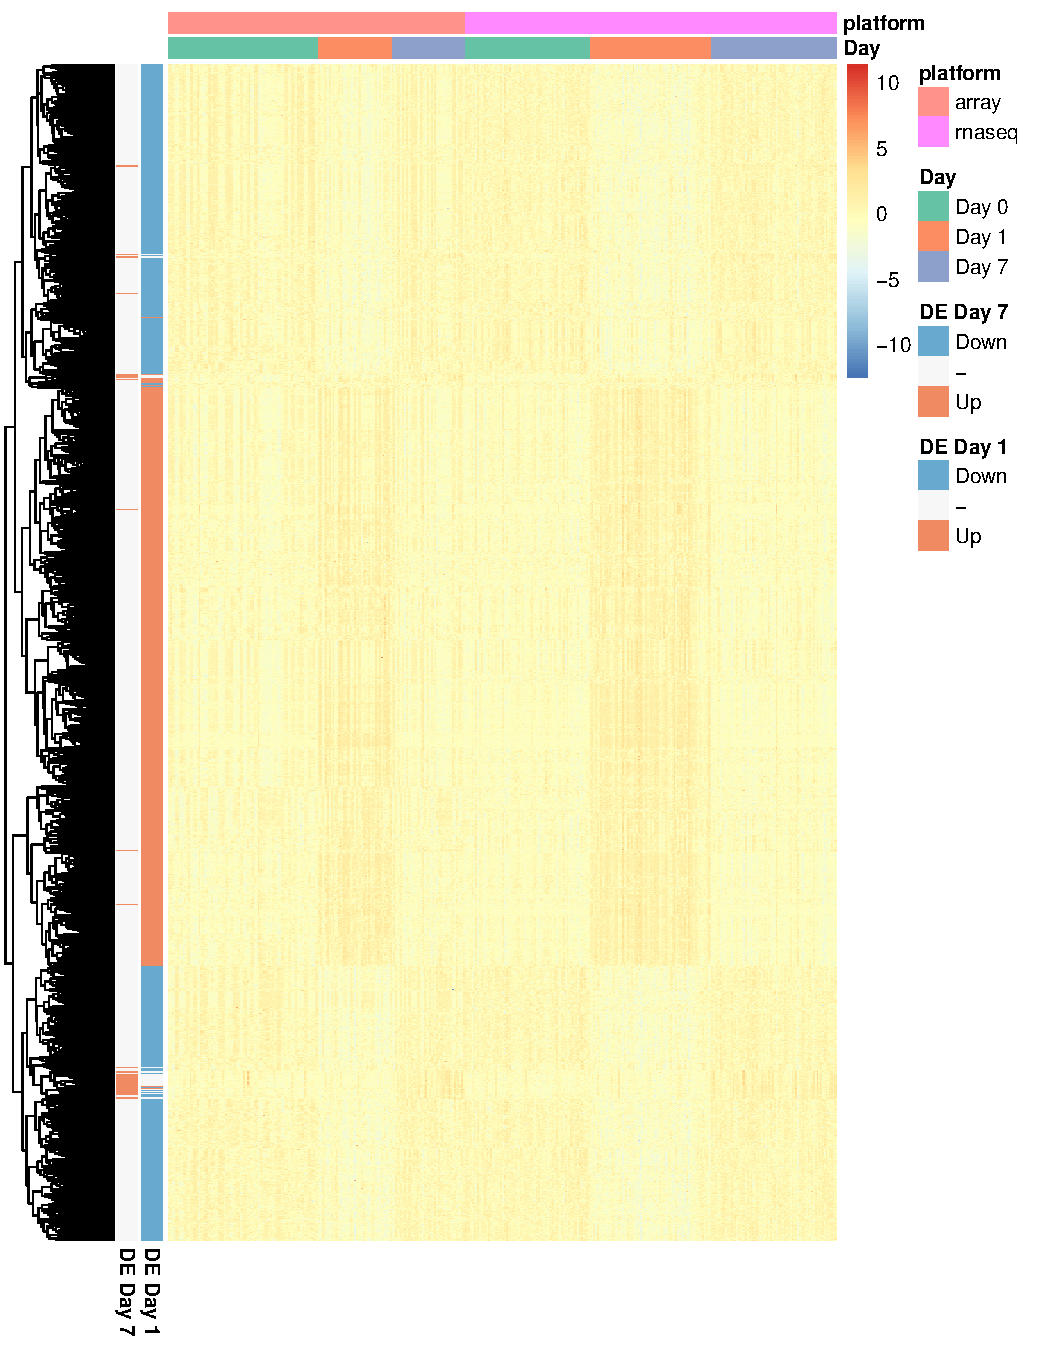
\includegraphics[width=1.0\textwidth]{mainmatter/figures/chapter_02/plot_dge_eqtl.heatmap_dge.pdf}
    \caption{Normalised gene expression for genes differentially expressed between any pair of timepoints ($\text{lfsr} < 0.05$, $\text{absolute fold change} > 1.5$) across \gls{HIRD} samples, clustered by gene (Manhattan distance metric).}
    \label{fig:hird_dge_heatmap}
\end{figure}

\subsection{Innate immune response at day 1 post-vaccination}

Consistent with global expression at day 1 being markedly different from expression at other timepoints (\autoref{fig:hird_expression_pcs}), the highest numbers of differentially expressed genes are observed at day 1, with 644 genes differentially expressed vs. baseline.
The majority of these (580/644) were upregulated.
The gene with the highest \gls{FC} increase at day 1 compared to baseline was \gene{ANKRD22} ($\log_2\text{\gls{FC}} = \num{4.489150}$), an interferon-induced gene in monocytes and \glspl{DC} involved in antiviral innate immune pathways\autocite{bin2016AnkyrinRepeatDomain}.
Other key genes in the interferon signalling pathway\autocite{schneider2014InterferonStimulatedGenesComplex} such as \gene{STAT1} ($\log_2\text{\gls{FC}} = 2.1693060$), \gene{STAT2}   ($\log_2\text{\gls{FC}} = 0.9489341$), and \gene{IRF9} ($\log_2\text{\gls{FC}} = 0.8153674$) are also upregulated at day 1.
Gene set enrichment analysis using \texttt{tmod} revealed that genes with the high \gls{FC} increases at day 1 were enriched in modules associated with activated \glspl{DC}, monocytes, toll-like receptor and inflammatory signalling (\autoref{fig:hird_tmodDotPlot_timepoint}), confirming that day 1 responses are dominated by signatures of innate immunity.
\todo{can also add MSigDB hallmark sets, which include interferon sets; and of course gene ontology sets}
64 genes were downregulated at day 1, enriched in modules associated with T cells and \gls{NK} cells, with the largest absolute fold change observed for \gene{FGFBP2} ($\log_2\text{\gls{FC}} = -0.9141547$).
\todo{not sure of interpretation at FGFBP2, it is indeed highly expressed in NKs through \url{https://dice-database.org/genes/FGFBP2}}
For both up and downregulated genes, there was a tendency to return to baseline expression levels by day 7.
\todo{any point in a table of e.g. top 20 DE genes, or is the gene set analysis already enough?}

\begin{figure}
    \includegraphics[width=1.0\textwidth]{mainmatter/figures/chapter_02/compare_dge_eqtl.tmodDotPlot.DGE.timepoint.pdf}
    \caption{Transcriptomic modules significantly up or downregulated post-vaccination. Size of circle indicates effect size. Color of circle indicates significance and direction of effect (red = upregulation, blue = downregulation).}
    \label{fig:hird_tmodDotPlot_timepoint}
\end{figure}
\todo{change x axis labels to baseline, specify top 10 procedure in figure caption}

\subsection{Adaptive immune response at day 7 post-vaccination}

59 genes were differentially expressed at day 7 vs. baseline, with expression fold changes more modest than those at day 1.
The genes with the highest upregulation were the B cell-associated genes \gene{TNFRSF17} ($\log_2\text{\gls{FC}} = 1.7538617$) and \gene{MZB1} ($\log_2\text{\gls{FC}} = 1.7369668$).
Plasma cell-specific genes including \gene{SDC1} (encodes CD138 \url{https://www.ncbi.nlm.nih.gov/pmc/articles/PMC5437827/}) ($\log_2\text{\gls{FC}} = 1.3673081$) and \gene{ELL2} (\url{https://www.nature.com/articles/ni.1786}) ($\log_2\text{\gls{FC}} = 0.8679659$) were also prominently upregulated.
\todo{finish citing}
Strongly enriched modules at day 7 were related to mitosis and cell proliferation, particularly in CD4\textsuperscript{+} T cells (\autoref{fig:hird_tmodDotPlot_timepoint}).
Both the CD4\textsuperscript{+} T cell and plasma cell response are indications of an adaptive immune response at day 7.

\subsection{Expression signatures associated with antibody response}

I also looked for genes which have expression associated with baseline-adjusted antibody response, as quantified by \gls{TRI}.
At the initial frequentist meta-analysis stage, with a significance threshold of $\text{\gls{FDR}} < 0.05$, 6 genes had expression associated with \gls{TRI} at baseline, 55 at day 7, and 11 pooling samples across timepoints (\autoref{fig:hird_DGE_effectSizeComparisons_rma}).
\autocite{sobolev2016AdjuvantedInfluenzaH1N1Vaccination} also identified genes with day 7 expression associated with antibody response, where response was defined as a binary phenotype based on 4-fold change (described in section \todo{add label}).
They reported 62 significant associations at \gls{FDR} $< 0.05$, of which 58/62 fall into the 13593 genes considered in my meta-analysis (circled, \autoref{fig:hird_DGE_effectSizeComparisons_rma}), and 15/58 replicated, all with the same positive direction of effect (high expression with high \gls{TRI}).
In the Bayesian meta-analysis, no single gene was detected as significantly associated with \gls{TRI} at $\text{\gls{lfsr}} < 0.05$ at any timepoint, or when pooling samples across all timepoints (\autoref{fig:hird_DGE_effectSizeComparisons_bayesmeta}).

\begin{figure}
    \includegraphics[width=1.0\textwidth,page=1]{mainmatter/figures/chapter_02/plot_dge_eqtl.DGE.effectSizeComparison.pdf}
    \caption{DGE effect sizes estimated in array vs. \gls{RNAseq}. Significance colored by frequentist random effects meta-analysis FDR < 0.05. Genes with day 7 expression associated with responder/non-responder status in \autocite{sobolev2016AdjuvantedInfluenzaH1N1Vaccination} are circled for that contrast.}
    \label{fig:hird_DGE_effectSizeComparisons_rma}
\end{figure}

\begin{figure}
    \includegraphics[width=1.0\textwidth,page=2]{mainmatter/figures/chapter_02/plot_dge_eqtl.DGE.effectSizeComparison.pdf}
    \caption{DGE effect sizes estimated in array vs \gls{RNAseq}. Significance colored by Bayesian random effects meta-analysis lfsr < 0.05. Genes with day 7 expression associated with responder/non-responder status in \autocite{sobolev2016AdjuvantedInfluenzaH1N1Vaccination} are circled for that contrast.}
    \label{fig:hird_DGE_effectSizeComparisons_bayesmeta}
\end{figure}

Significant enrichments were detected at the gene set level; the strongest effects are seen at day 7, where expression of cell cycle, CD4\textsuperscript{+} T cells, and plasma cells are associated with high \gls{TRI}.
At day 0, modules related with inflammatory response in myeloid cells are also associated with high \gls{TRI} (\autoref{fig:hird_tmodDotPlot_TRI}).

\begin{figure}
    \includegraphics[width=1.0\textwidth]{mainmatter/figures/chapter_02/compare_dge_eqtl.tmodDotPlot.DGE.TRI.pdf}
    \caption{Transcriptomic modules enriched in genes with expression associated with antibody response (\gls{TRI}) at each day. Size of circle indicates effect size. Color of circle indicates significance and direction of effect (red = expression positively correlated with TRI, blue = negative).}
    \label{fig:hird_tmodDotPlot_TRI}
\end{figure}
\todo{figure x labels here should be TRI, not R.vs.NR}

\subsection{Identifying expression signatures for predicting antibody response [probably cut this section and just add to discussion]}

\section{Discussion}

There is extensive transcriptomic response to Pandemrix vaccination in the \gls{HIRD} cohort.
Upregulation of genes and modules related to the interferon signalling pathway, monocytes, inflammatory response, and other aspects of innate immunity were detected at day 1.
This response is transient, with most such genes returning to baseline expression by day 7.
\todo{Not sure if there is a biological interpretion of downreg of T cells and NK cells gene sets at day 1, since it could be due to increase in other cell types in the sample. similar findings in \autocite{nakaya2016SystemsBiologyImmunity} though}
\todo{lit search for downregulation interpretation paper, and downreg T cell paper}
Upregulation of cell cycle/proliferation, activated CD4\textsuperscript{+} T cell, and B (plasma) cell genes and modules were detected at day 7.
This is likely a signature indicating the shift to an adaptive immune response, involving CD4\textsuperscript{+} T cell-supported differention and proliferation of antibody-secreting plasmablasts and plasma cells\autocite{murphy2016JanewayImmunobiology}.
These patterns of expression change between timepoints in the \gls{RNAseq} data are consistent with the patterns in the array data in the original study\autocite{sobolev2016AdjuvantedInfluenzaH1N1Vaccination}, and with expansions of monocyte and plasma cell populations seen in the \gls{FACS} data at days 1 and 7 respectively in the original \gls{HIRD} study\autocite{sobolev2016AdjuvantedInfluenzaH1N1Vaccination}.

In contrast, I was not able to fully replicate the originally reported single gene-level associations between day 7 expression and antibody response in the \gls{RNAseq} data and subsequent and meta-analyses.
In \autocite{sobolev2016AdjuvantedInfluenzaH1N1Vaccination}, 62 genes were reported as differentially expressed between vaccine responders and non-responders.
Although \autocite{sobolev2016AdjuvantedInfluenzaH1N1Vaccination} encodes responder status as a binary phenotype, whereas my analysis uses \gls{TRI}, this is not the primary difference, as 51/62 genes replicated (\gls{FDR} < 0.05) using \gls{TRI} when considering just the array data.
The same analysis using only the \gls{RNAseq} data replicated 0/62 genes.
\todo{might have to rerun everything using the original binary R/NR if this line of reasoning isn't strong enough}
\todo{move numbers to results?}
The majority of the effects for these genes were simply much stronger in the array dataset than in the RNAseq dataset (\autoref{fig:hird_DGE_effectSizeComparisons_rma}).
Given that the range of \gls{TRI} is higher in the array individuals (\autoref{tab:hird_table1}), this does not seem unusual that stronger \gls{TRI}-associated effects are observed there.
%
% \todo{TRI (cite) is a bit of a hack too to combine two assays. it seems to be 'residualised change score'}
% lots of issues in lit, see ch3 section
% \todo{also, see sorjonen2019PerilAdjustingBaseline change as predictor}
% should probably analyse MN, HAI, separately after log

58/62 reported hits were measured by both platforms and assessed in the meta-analysis.
Only 15/58 signals replicated using frequentist random-effects meta-analysis to combine per-platform estimates.
I do not consider these hits as robust, as the \gls{REML} estimate of between-platform heterogeneity was zero for 8563/13593 for the day 7 TRI contrast overall, and zero for all 15 of these signals.
None of these signals replicated in the Bayesian random-effects meta-analysis.
The Bayesian meta-analysis is in general more conservative, calling fewer differentially expressed genes compared to the frequentist analysis for all contrasts (\autoref{fig:hird_DGE_effectSizeComparisons_bayesmeta}).
Prior information about $\tau$ is incorporated, discouraging unrealistic estimates of zero heterogeneity.
Given the between-platform heterogeneity coming from both platform-specific technical differences and \gls{TRI} phenotype differences, relative to the modest effect size distributions compared to between-timepoint \gls{DGE} comparisons, the data are not well-positioned to identify significant single-gene associations with antibody response.
%
% Other caveats of the meta analysis
% - The very fact that a meta-analysis is performed adds some bias towards genes with fold changes that can be more consistently measured between platforms; these tend to be genes with higher expression.

% Did we choose the right phenotype?
%
% - the day 63 timepoint is late compared to many other studies
% - Nauta JJ, Beyer WE, Osterhaus AD. On the relationship between mean antibody level, seroprotection and clinical protection from influenza. Biologicals 2009; 37:216-21; PMID:19268607; http://dx. doi.org/10.1016/j.biologicals.2009.02.002 "In clinical studies seroprotection is normally defined as a specific antibody titer or antibody titer increase (seroconversion)."
% - other measures of seroconversion \url{https://www.who.int/biologicals/vaccines/Annex_2_WHO_TRS_963-3.pdf}
% - https://bmcinfectdis.biomedcentral.com/articles/10.1186/s12879-019-4049-5 Seroconversion may not correspond well to protection...

Expression signatures of antibody response were, however, observed at the gene set level, for modules of coexpressed genes that are associated with \gls{TRI} as a whole.
The strongest effects were observed at day 7, where expression of adaptive immune response modules (cell cycle, stimulated CD4\textsuperscript{+} cell, plasma cell modules) were positively associated with \gls{TRI}.
These are the same modules observed to be upregulated at day 7 compared to baseline; it seems that those individuals with the greatest antibody response to vaccination are most able to upregulate these gene sets by day 7 post-vaccination.

Module associations were also observed pre-vaccination (cell adhesion, enriched in B cells, proinflammatory cytokines, platelet activation), suggesting baseline immune state has some influence on long-term antibody response to Pandemrix.
%
% Day 1 TRI ?
% Inflammatory signatures of non-response
% https://www.jacionline.org/article/S0091-6749(17)31766-9/fulltext#sec2.4
% \enquote{The reduced efficacy of vaccination has also been linked to excessive inflammation for influenza,31 yellow fever,32 tuberculosis,33 and hepatitis B34 vaccines.}
%
Over the years, a diverse range of gene sets have been found to be baseline predictors of serological response to influenza vaccination:
    apoptosis\autocite{furman2013ApoptosisOtherImmune}; 
    Fc$\gamma$ receptor-mediated phagocytosis, TREM1 signaling\autocite{tsang2014GlobalAnalysesHuman};
    enriched in B cells, T cell activation\autocite{nakaya2015SystemsAnalysisImmunity};
    B cell receptor signalling, inflammatory response, platelet activation \autocite{hipc-chisignaturesprojectteam2017MulticohortAnalysisReveals}; 
several of which I also observe.
It should be noted that comparisons with these signatures from existing influenza systems vaccinology studies should caveated, as most existing studies are for non-adjuvanted influenza vaccines.
Adjuvanted influenza vaccines are considerably more immunogenic, and post-vaccination expression patterns differ to those of non-adjuvanted vaccines \autocite{sobolev2016AdjuvantedInfluenzaH1N1Vaccination,wilkins2017AS03MF59AdjuvantedInfluenza}.
\todo{could comment on phenotype differences too, i.e. HIRD measure antibodies at d63, much later than is popular in the field: d28 usually}
\todo{should probably emph sobolev didn't find prevacc signatures, and we did. But it's not exactly fair, as sobolev didn't use gene set enrichment as far as i can tell}
Hence, it is particularly important that the robustness of these observed baseline expression signatures be validated in an independent cohort for a comparable AS03-adjuvanted influenza vaccine.

%
% Sobolev:
% Of the volunteers analyzed, essentially all showed expansive changes in peripheral blood gene expression by day 1 (significant changes in ~9,000 gene probes (P < 0.05)) (Supplementary Fig. 2a), highly consistent with other studies that did not use adjuvants8,16,24,25.
% [...]
% In that regard, our study shows that the Pandemrix H1N1 vaccine provokes rapid and expansive, yet transient, activation of myeloid cells and effectors, similarly to changes induced by other vaccines, including flu vaccines lacking adjuvant8,13,15–17. However, our study also reveals a pronounced lymphoid contribution to the early phase of the immune response, most evident in the prominent transient upregulation of IFN-γ, which was not apparent in most other virus vaccine studies.
%
% As noted by \autocite{sobolev2016AdjuvantedInfluenzaH1N1Vaccination}, although the day 1 myeloid response was consistent with studies of non-adjuvanted seasonal influenza vaccines (e.g. \autocite{nakaya2011SystemsBiologyVaccination, bucasas2011EarlyPatternsGene, obermoser2013SystemsScaleInteractive}), the presence of interferon gamma-driven responses was unique to \gls{HIRD}.
% \todo{I think i did not mention specifically type II (IFN-g) in the results section. would need to add HALLMARK set CAMERA results to show this}
%
% Although it is known that AS03 does induce expression changes related to innate immune response at the injection site (\url{https://www.sciencedirect.com/science/article/pii/S0264410X11000399?via%3Dihub#sec0010}), the mechanism of action is unknown (\url{https://www.frontiersin.org/articles/10.3389/fimmu.2017.01760/full}), and there have been relatively few studies of the effect of AS03 or AS03-adjuvanted vaccines on the \gls{PBMC} immune transcriptome aside from the \autocite{sobolev2016AdjuvantedInfluenzaH1N1Vaccination} study itself.
%
% https://www.sciencedirect.com/science/article/pii/S1879625711000769?via%3Dihub#bib0180
% Their mechanism of action remains incompletely understood, however they may amplify immune responses by enhancing antigen presentation and recruiting inflammatory cells to the area of antigen deposition (reviewed in [36]).
%
% https://link.springer.com/article/10.1007/s10875-010-9490-6
% Immune responses to inactivated influenza virus adjuvanted with a different oil-in-water emulsion, MF59, have recently been described [35, 36]. Although a direct comparison between the adjuvants is complicated by the fact that different methodologies may have been used to measure immune responses, our data indicate that AS03A-adjuvanted influenza vaccines induce strong HI responses and CD4 T-cell frequencies relative to those induced with the MF59-adjuvanted product.
%
% AS03-adjuvanted split-virion influenza A/H5N1 vaccine: (\gene{GBP1}, \gene{IRF1}, and \gene{STAT1}) expressions are up in adjuvanted (\url{https://journals.plos.org/plosone/article?id=10.1371/journal.pone.0167488}), three genes that play a role in interferon and antiviral response.
%
% A study of the MF59-adjuvanted \gls{TIV} \autocite{nakaya2016SystemsBiologyImmunity}
%

%
% Sobolev:
% In sum, neither molecular nor cellular data offered any consensus prevaccination predictor of nonresponsiveness akin to those proposed in studies of nonadjuvanted vaccines8,16,17,24,31.
%
% We find some, but...
% - The utility of such signatures is unclear.
% - diagnostics would require prediction
% - and would require protection, not immuno
%
% TODO
\todo{There is also something to be said about 'prediction is not inference'. For use as correlates of protection, as promised by proponents of systems studies, prediction is what is important.}
% - Prediction is not inference tsang2014GlobalAnalysesHuman
% TODO: https://stats.stackexchange.com/questions/22718/what-is-the-difference-between-linear-regression-on-y-with-x-and-x-with-y/62323#62323
% In statistics, errors-in-variables models or measurement error models[1][2][3] are regression models that account for measurement errors in the independent variables. In contrast, standard regression models assume that those regressors have been measured exactly, or observed without error; as such, those models account only for errors in the dependent variables, or responses.[citation needed]
% controlled by experimenter
% In statistics, errors-in-variables models or measurement error models[1][2][3] are regression models that account for measurement errors in the independent variables. In contrast, standard regression models assume that those regressors have been measured exactly, or observed without error; as such, those models account only for errors in the dependent variables, or responses.[citation needed]
% https://web.stanford.edu/class/polisci100a/regress5.pdf
%
% For prediction, what rules can be easily implemented in the clinic?
% DAMIP gives rulesets composed of small sets of genes, amenable to rapid qPCR assays.
% We can model HAI and MN in split models. No change scores required.

% Seasonal can prime for H1N1
%
% \2 Efficacy, dosing: \enquote{...a single dose of monovalent 2009 H1N1 vaccine was recommended in adults, but young children were recommended to receive 2 doses (reviewed by [3••]). It is likely that a single dose was sufficient to induce immunity in adults because prior exposure to seasonal H1N1 viruses had immunologically primed the population.}
%
% "Seasonal influenza vaccine provides priming for A/H1N1 immunization." \url{https://www.ncbi.nlm.nih.gov/pubmed/20371459}
%
% Demonstration in a mouse model: \url{https://www.ncbi.nlm.nih.gov/pmc/articles/PMC3024675/}
%
% \2 Inclusion of H1N1 strains into seasonal vaccines
% Sobolev sampled in March 2010 to August 2011
% \2 Later cohorts may have recall response to H1N1 from seasonal vaccination

% TODO: compare to seasonal

% - Overall conclusions.
In conclusion, Chapter 2 characterises the expansive changes in \gls{PBMC} gene expression that follow vaccination with Pandemrix.
The dominant trend for all individuals is transient upregulation of the innate immune response at day 1, transitioning into adaptive immunity by day 7.
Baseline-adjusted antibody response is correlated with expression of gene sets, particularly adaptive immunity modules at day 7, but also for some modules pre-vaccination.
Unfortunately, between-platform variation in expression impedes identification of specific genes that contribute.
The fundamental question of why gene expression and antibody responses vary between \gls{HIRD} individuals remains.
Chapter 3 will examine one hypothesis: the impact of common human genetic variation on Pandemrix expression response.
% TODO: ch4 also corrects for cell props
\todo{At no point in this chapter are we estimating causal effects: add point on why not CIT (lower n than franco)}
\todo{found signatures, but so what? Feels like chapter lacks a punchline?}

% TODO: not adjusted for cell comp, but not necc bad

% TODO: add a whilst we were not able to X in the intro, the field has advanced by Y, future Z needed
 % HIRD transcriptomics
%
% Chapter 3
%
% Response eQTL-style paper

\chapter{Genetic factors affecting Pandemrix vaccine response}
\label{chap:hird_reQTL}

\section{Introduction}

\subsection{Genetic factors affecting influenza vaccine response}

- Vaccine-induced antibody response is a complex trait.
% Impact of host genetic polymorphisms on vaccine induced antibody response
% https://www.ncbi.nlm.nih.gov/pmc/articles/PMC4962936/#!po=22.7273
% Table 1.
% Genes with polymorphisms that influence the vaccine induced antibody level (selected studies).
% Individuals carrying the minor allele in one or both alleles showed an increased seroconversion rate after influenza vaccination.62
% Further SNPs that influence the humoral immune response to influenza vaccination have been reported (see Table 1):

Specifically for response to seasonal influenza vaccines...
% Start here with this review
% 2019
% Host Factors Impact Vaccine Efficacy: Implications for Seasonal and Universal Influenza Vaccine Programs
% https://jvi.asm.org/content/93/21/e00797-19

% 2004
% HLA-DRB1*0701 allele was over represented among persons who fail to mount a neutralizing antibody response.
% https://www.ncbi.nlm.nih.gov/pubmed/15462607

% 2008
% Immunogenetics of Seasonal Influenza Vaccine Response
% https://www.ncbi.nlm.nih.gov/pmc/articles/PMC2610683/

% 2019
% Common Genetic Variations Associated with thePersistence of Immunity following ChildhoodImmunization
% https://www.cell.com/cell-reports/pdf/S2211-1247(19)30682-5.pdf

% Stretch?
% Also
% Prevacc signatures of Tri
% Using larger transcriptomic dataset
% Are they genetic

\subsection{\Glsfmtlongpl{reQTL} for seasonal influenza vaccination}

A potential mechanism through which genetic variation can affect vaccine response is through altering the expression of genes.

eQTLs have condition specificity
e.g. cell types or tissues

A reQTL is: \autocite{vandiedonck2017GeneticAssociationMolecular}
% An important kind of eQTLs, called response eQTLs (reQTLs), occurs following
% exposure to an external signal (Table 2), in particular in the immune system in
% response to infectious agents and to various stimuli.49, 54, 55 Other
% environmental factors, including hormones, drugs, diet, metals or pollutants,
% can also be the source of reQTLs.56
- an eQTL becomes more or less important after perturbation: Tells you something about the mechanism of perturbation.
- Either expression regulatory activation/repression (signalling cascade -> TFs, chromatin remodelling etc.)

Little work done on reQTL for vaccine stimulation
Summarise Franco et al
In the case of inactivated trivalent influenza vaccine, genetic variation in membrane trafficking and antigen processing genes was associated with both transcriptomic and antibody responses in patients after vaccination [Franco].

\subsection{Chapter summary}

% NOTE:
% Narcolepsy controversy (more evidence for genetic interaction with Pandemrix vaccine response in particular)

- In \autoref{chap:hird_DGE}, we observed massive changes in gene expression longitudinally after Pandemrix vaccination, as well as expression signatures correlated to degree of antibody responses.
[variation observed in response to Pandemrix, e.g R vs. NR trajectories]
- How does host genetics affect response to Pandemrix in the HIRD cohort?

Sobolev pros
    Small effect expected?
    More variation will usually be explained by history of exposure rather than genetics, so may be harder to detect.
    but not here

also Knowns
    Sobolev: R vs NR, 
    inconsistent variation in why people are NR

In this study, we model the influence of host genetics on longitudinal transcriptomic and antibody responses to Pandemrix, in vivo.
    overall strat: map per timepoint, joint analysis
    call reqtls
    characterise
% have abs
    % not that we use
% [main aim: how much variation in response is genetic?]
    % not that we calc
% [other aims: assess differences to seasonal influenza vaccines]
% [summary of main results]
% Utility of genetics: allows coloc

\section{Methods}

\subsection{Overall strategy for detecting reQTLs}

% TODO: start here. text!

for reQTL
it may also seem natural
overall Why not mapping on deltas? (if we are interested in the direct question of G on change)
    ackermann: change scores are prone to increased noise
    from franco: "We attempted analyses with an approach similar to that proposed by the reviewers in the course of our work, but found that the approach that was ultimately chosen to explore the day differences was the most powerful. Specifically, utilizing a pairwise comparison (difference) between time points as the substrate for the eQTL analysis would lead to an increase in the technical variance of the phenotype, as the sum of two independent (technical) errors has twice the variance of an individual measurement. "

instead within timepoint, and compare effects
if change in expression vs d0 is under genetic control, we should see change in effect size of eqtl vs d0
can do this because genotype can be assumed to be constant across timepoints

It can be a tricky business to define response eQTLs, or indeed any condition specific eQTLs
    early attempts
    naive
    map condition by condition
    signif

why joint
In the same period that condition specific eQTL mapping was getting started (as discussed in section...), tools were being created to identify these locitools were being created to identify these loci
review: condition/Cell-type specific methods
refere to 2019-11-19 Cell-count specific eQTL mapping papers
PANAMA, LIMMI

%
% Restricted to non-full Bayesian methods.
%
% See last paragraph of discussion in
% Kontopantelis, E., Springate, D. A., & Reeves, D. (2013). A Re-Analysis of the Cochrane Library Data: The Dangers of Unobserved Heterogeneity in Meta-Analyses. PLoS ONE, 8(7), e69930. https://doi.org/10.1371/journal.pone.0069930
% For small k, Sidik MVa or Ruhkin RBp recommended.
%
% metafor manual
% If, instead of the crude estimate, one wants to use a better apriori estimate, one can do so by passing this value via control=list(tau2.init=value)
% Sidik-Jonkman estimator, also called the ‘model error variance estimator’, is implemented in metafor (SJ method).
% Starts with an init estiamte of ri=sigma2i/tau2i i.e. ratio of study-specific and between-studies het variance, then updates.
% They recommend using Hedges [1], to init, but this is bad???
% We use mode of gamma as an apriori estimate of tau.
%
% 2.7.	Meta-analysis with metafor
% 2.7.1.	Per day, use rma(‘REML’) to fit random-effects model on association beta and beta_ste, per gene-SNP pair, using all timepoints from array/RNA-seq for that day
% 2.8.	eigenMT to get number of independent tests per gene
% 2.8.1.	split previously generated geneloc and snpsloc by chrom
% 2.8.2.	per chrom, run eigenMT on limix output (arbitrary day, since the set of snps cis to each gene does not vary by day)
% 2.9.	Compute hierarchical FDR
% 2.9.1.	Per day
% 2.9.1.1.	Use eigenMT estimates to apply local Bonferroni per gene
% 2.9.1.2.	Compute global BH FDR

Finally
recall hird has multi datasets and measures within each timepoitn

why mega?
    can't bayesmeta, which would be ideal.
    also, small n for array


\subsection{Mapping cis-\glsfmtlongpl{eQTL} with \glsfmtlongpl{LMM}}

As discussed in \autoref{chap:hird_DGE}, the \gls{HIRD} cohort is multi-ethnic, and population structure can affect gene expression\autocite{brown2018ExpressionReflectsPopulation}.
I addressed this by treating the top \glspl{PC} of the genotype matrix as covariates for large-scale population structure (ancestry).
In the context of \gls{eQTL} mapping, where the aim is to assess the marginal effect of a single genetic variant on expression, it is even more important that the confounding effect of population structure is accounted for.

% This is great background/intuition: golan2018MixedModelsCaseControl
% using LMMs is appropriate for controlling for population structure (which is a common
% problem in human GWAS), as well as for cryptic relatedness, and that LMMs outperform
% the previously preferred principal component analysis (PCA) approach in addressing these
% issues (Yang et al., 2014).
%
% Also see: 2018-11-26 notes in log
For genetic association studies, an appealing approach is the \gls{LMM}, which includes a random effect that directly models genetic correlation between individuals as the covariance of that random effect\autocite{price2010NewApproachesPopulation, eu-ahsunthornwattana2014ComparisonMethodsAccount, golan2018MixedModelsCaseControl}
The \gls{LMM} approach has the advantage of not only modelling large-scale population structure, but also cryptic relatedness (the presence of closely related individuals in a sample assumed to consist of unrelated individuals\url{https://projecteuclid.org/euclid.ss/1271770342}) from finer-scale effects such as family structure\autocite{golan2018MixedModelsCaseControl}.
\todo{add some indication of how much inflation is reduced by LMMs}

\subsubsection{Estimation of kinship matrices}

% 1.	Build GRM using LDAK 5
% 1.1.	Start with pre-imputed genotypes coreex_eQTLflu_20171204.gencall.smajor.impute_sex.qc6
% 1.1.1.	“Estimates of SNP heritability are very sensitive to genotyping errors”, so we can’t use imputed SNPs without filtering for high INFO.
% 1.2.	Prune to MAF 0.05, autosomes only
% 1.3.	Compute LDAK SNP weightings
% 1.4.	Compute kinships for each chromosome
% 1.5.	Join per-chromosome kinships into genome-wide kinships
% 1.5.1.	Use the leave-one-chromosome-out strategy

- The LMM requires a kinship matrix to scale(?) the covariance matrix of the random effect
- When testing a variant for association, to avoid loss of power from 'proximal contamination', kinship matrix used should not include that variant\url{https://www.ncbi.nlm.nih.gov/pmc/articles/PMC3597090/}.
- A simple way to avoid this is to compute \gls{LOCO} kinship matrices from all variants on chromosomes other than that variant's chromosome\autocite{lippert2011FaSTLinearMixed}.

I estimated kinship in the \gls{HIRD} data from common autosomal variants, using \texttt{LDAK} (5.0), which computes kinship matrices adjusted for bias caused by \gls{LD}\autocite{speed2012ImprovedHeritabilityEstimation}.
Filtered, pre-imputation sample genotypes from \autoref{subsec:hird_DGE_methods_genotypePhasingAndImputation} were pruned to $\text{\gls{MAF}} > 0.05$.
A kinship matrix was computed for each autosome, then combined into a single genome-wide matrix using \texttt{LDAK -{}-join-kins}.
To obtain a \gls{LOCO} kinship matrix for each autosome, each autosome's kinship matrix was then subtracted from this genome-wide matrix (\texttt{LDAK -{}-sub-grm}).
- The \gls{LOCO} kinship matrix excluding chromosome 1 is shown [...]

\missingfigure{chr1 loc kinship matrix as example, note the estimates for self-relatedness on the diagonals are not constrained to be 1.}

% Full notes about cell type correction pipeline rationale at 2019-10-30 in log
\subsubsection{Estimation of cell type abundance via expression deconvolution}

As \gls{PBMC} samples are a mixture of immune cells, and a fixed input of RNA extracted from that mixture is used to estimate expression, bulk estimates for genes that have cell type specific expression depend on the relative proportions of each cell type in each sample.
% Also, \gls{RNAseq} expression estimates are inherently compositional \url{https://www.ncbi.nlm.nih.gov/pubmed/29608657} \url{https://academic.oup.com/gigascience/article/8/9/giz107/5572529}.

% E.g. Davenport 2018: “observed eQTL interactions could be the consequence of a cellular subpopulation whose frequency is being altered by the environmental perturbagen or variability in cell type proportions between individuals.”
% “inferred the relative proportions of nine hematopoietic populations from the RNA-seq data using CIBERSORT”
% After correcting for cell proportions “reduction in significant interactions suggests that some of these interactions may be related to changes in cell proportions”
- G is constant. C is not constant
- It is well known that QTLs can be cell type specific, due to cell type specific expression and other mechanisms (fu)
- Cell proportions change after vacc, reQTLs calls can be confounded if cell type abundances are not taken into account.
- If it is assumed that eQTL effects can differ between cell types, then in addition to the genotype main efect, an interaction term between genotype and cell type abundance is required.

- Need an estimate of abundance.
- I do not have FACS data for all samples in HIRD, only subset of array individuals.
% Related:
% Westra, H.-J., Arends, D., Esko, T., Peters, M. J., Schurmann, C., Schramm, K., … Franke, L. (2015). Cell Specific eQTL Analysis without Sorting Cells. PLOS Genetics, 11(5), e1005223. https://doi.org/10.1371/journal.pgen.1005223
% Gets cell type estimates from proxy genes
- Expression deconvolution is a viable alternative.
- Chose xCell, as used by the GTEx paper, which works by... e.g. spillover etc. ... returns enrichment scores which are not... only uses about 10k genes
- xCell includes signatures for 64 cell types, but recommends cell types not be included if not expected to be present.
% See 2019-11-14 log
% https://link.springer.com/chapter/10.1007/978-3-319-16104-4_15
% https://www.nature.com/articles/s41588-018-0089-9
% www.blueprint-epigenome.eu/index.cfm?p=7BCEDA45-EC73-3496-2C823D929DD423DB
Reviewing the literature to find broad classifications for peripheral blood cell types also present in the \gls{PBMC} compartment\autocite{davenport2018DiscoveringVivoCytokineeQTL},
I settled on 'CD4+ T-cells', 'CD8+ T-cells', 'B-cells', 'Plasma cells', NK cells, Monocytes and DCs.

xCell applied to expression data 
% /nfs/users/nfs_b/bb9/workspace/phd/output/hird/rnaseq/4_de/array/array_data_setup.y.filtered.MaxMean.combat.rds
% and /nfs/users/nfs_b/bb9/workspace/phd/output/hird/rnaseq/4_de/array/array_data_setup.sample.metadata.merged.rds
As xCell is rank-based, no additional xforms.
rnaseq and array separate

- xCell enrichment scores scaled and centered, 
- Scale all timepoints together, so that a value of 0 cell proportion effect represents the same thing across all timepoints

\begin{figure}
    \centering
    \includegraphics[width=1.0\textwidth,page=1]{mainmatter/figures/chapter_03/get_xCell_estimates.dataset_array.plots.pdf}
    \caption{xCell enrichment scores in array data}
    \label{fig:hird_xCell_scores_heatmap_array}
\end{figure}

\begin{figure}
    \centering
    \includegraphics[width=1.0\textwidth,page=1]{mainmatter/figures/chapter_03/get_xCell_estimates.dataset_rnaseq.plots.pdf}
    \caption{xCell enrichment scores in rnaseq data}
    \label{fig:hird_xCell_scores_heatmap_rnaseq}
\end{figure}

- The xCell estimates are correlated.
- select top ones that are reasonable uncorrelated
- in each case 3 pcs pass eigenvalue > 1 rule of thumb
- PCA them
PCs are orthogonal (and thus linearly independent)
but for intepretability
- select top 3 cell types with close cos2
    - they are also top cells that changed in sobolev


\begin{figure}
    \centering
    \begin{subfigure}[b]{0.49\textwidth}
        \centering
        \includegraphics[width=1.0\textwidth,page=8]{mainmatter/figures/chapter_03/get_xCell_estimates.dataset_array.plots.pdf}
        \caption{array}
    \end{subfigure}%
    \hfill%
    \begin{subfigure}[b]{0.49\textwidth}
        \centering
        \includegraphics[width=1.0\textwidth,page=8]{mainmatter/figures/chapter_03/get_xCell_estimates.dataset_rnaseq.plots.pdf}
        \caption{rnaseq}
    \end{subfigure}%
    \caption{xCell cos2 contributions}
    \label{fig:hird_xCell_loadings}
\end{figure}


% NOTE:
% Why impute for cell counts but not for expression data?
% - expression matrices are mostly complete, and we only exclude genes based on low expression in RNAseq
% - we cannot drop whole FACS panels so easily like we can drop genes
- Validate estimates on subset with FACS data.

-    group raw data by panel and cell type
-    Rank-Based Inverse Normal Transformation
    % PHEASANT https://www.biorxiv.org/content/biorxiv/early/2017/02/26/111500.full.pdf and
    % Astle 2016, both use this method.
- then imputewithmissForest


- plot against xcell estimates
- kinda moderate, esp at day1

\begin{figure}
    \centering
    \begin{subfigure}[b]{0.43\textwidth}
        \centering
        \includegraphics[width=1.0\textwidth,page=6]{mainmatter/figures/chapter_03/validate_xCell_estimates.cell_type_pairs.pdf}
        \caption{mono}
    \end{subfigure}%
    \vspace{1em}\vfill%
    \begin{subfigure}[b]{0.43\textwidth}
        \centering
        \includegraphics[width=1.0\textwidth,page=3]{mainmatter/figures/chapter_03/validate_xCell_estimates.cell_type_pairs.pdf}
        \caption{nk}
    \end{subfigure}%
    \vspace{1em}\vfill%
    \begin{subfigure}[b]{0.43\textwidth}
        \centering
        \includegraphics[width=1.0\textwidth,page=2]{mainmatter/figures/chapter_03/validate_xCell_estimates.cell_type_pairs.pdf}
        \caption{plasma}
    \end{subfigure}%
    \caption{xCell vs facs int}
    \label{fig:hird_xCell_vs_FACS}
\end{figure}

\subsubsection{\glsfmtshort{eQTL}-specific expression preprocessing}

There are a wide range of transformations that are often applied to expression data before \gls{eQTL} mapping.

e.g. Rank-based int:
% 2018-03-15 in log details the GTEx pipeline.
heavily used in eqtl, e.g GTEX \url{https://storage.googleapis.com/gtex-public-data/Portal_Analysis_Methods_v7_09052017.pdf}
    Although criticised: "Rank-Based Inverse Normal Transformations are Increasingly Used, But are They Merited?"

e.g. Z
\url{https://github.com/molgenis/systemsgenetics/wiki/eQTL-mapping-analysis-cookbook-(eQTLGen)}

- outliers
- normality also: genomic data: resid normal is mostly defined by input normal

- Considering my main goal is to find reQTLs
I performed simulations to evaluate the effect of the transformation on reQTL calls

sim reQTLs on the log scale with specific betas
define strength as diff

scale only
2 and 4 sim to have same relative effect size change
2 and 4: betas are 0 1, 1 2
after, 0 0.75, 0.4, 0.8

only center
both
do not induce fals negs
preserve both rel egene str

but no point, since intercept is included

in the end, no scale
extra careful on outliers

\begin{figure}
    \centering
    \includegraphics[width=1.0\textwidth,page=1]{mainmatter/figures/chapter_03/simulate_expression_transforms.pdf}
    \caption{expression xforms}
    \label{fig:hird_eQTL_expressionTransform_sims}
\end{figure}

\subsubsection{Finding hidden confounders using factor analysis}

% 2.	Infer global confounders by detecting hidden factors affecting expression with PEER
% 2.1.	“batch effects and other global confounders reduce the power to find expression quantitative trait loci”
% 2.1.1.	“We assume that these variables have a broad influence, and thus each of them has an effect size for every gene.”
% 2.1.2.	“The learned variables can be constrained to affect known sets of genes via a prior connectivity matrix. By default, with no prior connectivity given, they are assumed to be global and to affect large fractions of all genes“
% 2.1.3.	Note that due to this assumption: “If large trans hotspots are dominating, associations may get erroneously explained away as confounding factors”
% 2.2.	Round input expression to integer counts
% 2.2.1.	Input is y: the scaledTPM (TPM's scaled up to library size) from tximport.
% 2.3.	Normalise for library size and variance stabilize with varianceStabilizingTransformation from DESeq2 (recommended in PEER paper)
% 2.3.1.	Vst is like a souped up log: “In all cases, the transformation is scaled such that for large counts, it becomes asymptotically (for large values) equal to the logarithm to base 2 of normalized counts.”
% 2.3.2.	Note we cannot use voom-ed expressions from the DGE pipeline, as there are some samples missing due to lack of Ab titre data
% 2.3.3.	Do not blind the transformation to experimental design matrix: “If many of genes have large differences in counts due to the experimental design, it is important to set blind=FALSE for downstream analysis.”
% 2.3.4.	Here we use a simple design matrix of groups defined by all combos of day x R/NR
% 2.4.	Run PEER by timepoint
% 2.4.1.	Match GTeX pipeline: https://github.com/broadinstitute/gtex-pipeline/tree/63b13b8ced25cf8ab8e7a26f40a495e523630a9b/qtl , with some modifications.
% 2.4.1.1.	Note this pipeline uses quantile normalized, rank INT transformed expression, as PEER input
% 2.4.2.	Quantile normalize the samples with preprocessCore::normalize.quantiles
% 2.4.2.1.	Causes the expressions of the samples to have the same empirical distribution
% 2.4.2.2.	i.e. the the highest expression in each sample is set to the mean of the highest values of all samples, and in the case of no tied values, each sample’s expressions becomes a permutation of each other sample’s
% 2.4.3.	Standardize expression of each gene with Rank-Based Inverse Normal Transformation
% 2.4.3.1.	i.e. rank the expressions of a gene, then replace with values from the standard normal e.g. > rank.based.INT(1:5, c=3/8): [1] -1.1797611 -0.4972006  0.0000000  0.4972006  1.1797611
% 2.4.4.	Setup and run PEER
% 2.4.4.1.	Allow up to 10k iterations, start with n.samples/4 PEER factors
% 2.4.4.2.	One can include known covariates. We don’t, as it causes weird things like PEER factors not being sorted in descending relevance
% 2.4.4.2.1.	~ 1 + batch + rna.conc + Gender + Age.at.vaccination..years. + PC1.imputed + PC2.imputed + PC3.imputed + PC4.imputed
% 2.4.4.2.2.	Note this includes an intercept that represents the mean expression

myriad of other fx are not constant

PEER

% If RANKINT, why RANKINT before PEER?
%
% Are your covariates under control? How normalization can re-introduce covariate effects
% https://www.ncbi.nlm.nih.gov/pubmed/29706643
% "Many statistical tests rely on the assumption that the residuals of a model are normally distributed [1]. In genetic analyses of complex traits, the normality of residuals is largely determined by the normality of the dependent variable (phenotype) due to the very small effect size of individual genetic variants [2]. However, many traits do not follow a normal distribution."
% "applying rank-based INT to the dependent variable residuals after regressing out covariates re-introduces a linear correlation between the dependent variable and covariates, increasing type-I errors and reducing power."


% Trans-eQTLs Reveal That Independent Genetic Variants Associated with a Complex Phenotype Converge on Intermediate Genes, with a Major Role for the HLA
% https://doi.org/10.1371/journal.pgen.1002197
%
% In order to increase the number of detectable cis- and trans-eQTLs we applied a
% principal component analysis (PCA) on the sample correlation matrix. We, among
% others [19], [20], argue that the dominant PCs, capturing the larger part of
% the total variation, will primarily capture sample differences in expression
% that reflect physiological or environmental variation as well as systematic
% experimental variation (e.g. batch and technical effects).
% [...]
% An aspect to consider is that with
% the removal of more PCs from the data, the degrees of freedom of the data will
% decrease. Furthermore, it is not immediately clear which PCs will actually
% capture physiological, environmental, and systematic variation, which might
% lead to removal of genetically determined expression variation as well.
% Therefore a tradeoff has to be made on the number of PCs to subtract from the
% data.
% - subtracted 50 PCs for cis, 25 PCs for trans.

expression PCs: if too many, will explain away the signal
Not a problem with cis-eQTLs, but trans might have more global effects
    GWAS on PEER factors would pick up trans fx, cell count QTL effects
Unlike PCs, PEER factors are not constrained to be orthogonal: adding more and more factors will not explain more of the variance
    Also, they are weighted with ARD 
    results is that variance of output factors declines to zero

start with COUNT Data

convert to log scale and var stab
RNAseq only
% vsd <- vst(dds.filtered, blind=F)
mega
% vsd <- ComBat(dat=vsd, batch=sample.metadata.merged$batch, par.prior = T)
vsd is a log with shrinkage for low counts
also corrects for depth between sampline norm

gender, 4pcs, 3 cell types
explicit inclusion, peer finds additinal k

why include genetic PCs
see stegle 2012 PEER paper: if PCs are not included, they can be recapitulated in the factors
% (e.g., by introducing principal components of the genotype data), is not included in the model, and it may be recapitulated in the inferred factors.

\subsubsection{\glsfmtshort{eQTL} mapping per timepoint}

% 2.5.	Preprocess genotypes for limix
% 2.5.1.	Convert MAF filtered VCF -> 012 -> hdf5 format
% 2.5.1.1.	Do this for both strict 012 and continuous dosages
% 2.5.2.	Also convert 012 -> matrix eqtl SNP matrix format
% 2.5.2.1.	For eigenMT
% 2.5.3.	Parse out snpinfo and snplocs from VCFs
% 2.5.3.1.	Snpinfo for snp ids, for limix
% 2.5.3.2.	Snplocs for snp positions, and eigenMT
% 2.6.	Map eQTLs using limix 2.0, per timepoint
% 2.6.1.	Map cis-eQTLs within +- 1Mb of the gene start
% 2.6.1.1.	Phenotypes: per timepoint normalised input.expr from PEER script
% 2.6.1.2.	Covariates: sex, batch, 4 genotype PCs, 4 PEER factors
% 2.6.1.3.	Genotypes: MAF > 0.10 (in whole 169 individuals)
% 2.6.1.4.	Kinship: from LDAK, leave-one-chrom-out
% 2.6.2.	Output results in matrix eqtl-like output format

% For list of various methods considered, also see 2018-03-05, 2018-07-25, 2018-07-27 etc. in log
The performance of various software implementations of \glspl{LMM} specialised for genetic association studies are highly comparable; the specific choice of implementation can usually be made on the basis of computational efficiency\autocite{eu-ahsunthornwattana2014ComparisonMethodsAccount}.

choose the covariates approach, not residuals
    % Bias due to two‐stage residual‐outcome regression analysis in genetic association studies https://doi.org/10.1002/gepi.20607
    why including known covariates: why not a two stage approach?

    as sample size is modest, keep dfs correct
    how to choose number?

\begin{figure}
    \centering
    \includegraphics[width=1.0\textwidth,page=1]{mainmatter/figures/chapter_03/count_eGenes.signif_eGenes_vs_PEER_n.dataset_mega.chr_chr1.pdf}
    \caption{optimlise}
    \label{fig:hird_neGenesvsPeerK}
\end{figure}

var filters

    Sample AC thresh
        note they are dosages. if they were not, use ac thresh to estimate number of hom minor expected

    Partial justification for not considering sex chromosomes
    % https://www.nature.com/articles/ng.467
    % As is standard for imputation, we excluded all X-linked SNPs for the following reasons: (i) the X chromosome has to be treated differently from the autosomes; (ii) it cannot be predicted which allele is active on the X chromosome, (iii) testing males separately from females results in different sample sizes and power. Imputation of SNPs in the HapMap CEU population was performed using either MACH46 or IMPUTE47. All SNPs with a MAF <0.01 were excluded from analysis. In total, up to 2.11 million genotyped or imputed SNPs were analyzed.

Post-impuation, Genotypes are probabilities
    Genotypes were converted to dosages using bcftools (1.7-1-ge07034a)

The final model:

% sample_AC_thresh 15
% cis_dist 1e6
% cis only

% x genes

\subsection{Joint \glsfmtshort{eQTL} analysis across timepoints}

% 2.10.	mashr
% 2.10.1.	Apply mashr to per-day meta-analysis beta/beta_ste results

Simple, mixed models, joint models, multilocus models; Ending with why we chose mashr
used for smoothing, info sharing, fdr
    normally eqtls use perms for FDR
mashr beats out stuff it compared to in the paper e.g. metasoft

fit model

Choice of strong effects
If there is a particular condition with much greater power, choosing the lowest p value for each gene across all conditions could bias strong effects towards including just condition-specific effects for that particular condition.
how to ensure condition specific effects are present? look at heatmap of strong subset

correlations
    we dont' give up repeat measures strenght

compute posteriors

lfsr:
% type s error rates for classical and bayesian single and multiple comparison procedures
% WhyWe (Usually) Don’t Have to Worry About Multiple Comparisons (2012)
% Beyond Power Calculations: Assessing Type S (Sign) and Type M (Magnitude) Errors (2014)
% Stephens, M. (2016). False discovery rates: A new deal. Biostatistics, kxw041. https://doi.org/10.1093/biostatistics/kxw041

\subsection{Defining shared and response eQTLs}
% See notes from 2018-10-11 on wald test, and comments on sharing_func in get sharing script

mash suggests, but limitations
% # We define two effects to be shared in sign if they
% # have the same sign; we define them to be shared in magnitude if they also have an
% # effect within a factor of 2 of one another.
% # When computing sharing between tissues r and s, we consider only
% # QTLs that are significant (lfsr < 0.05) in at least one of r and s. This is to avoid
% # sharing estimates being driven by estimates of null or nearly null effects.

beta-comparison approach from Sarah Kim-Hellmuth 2017
% 7 conditions, pairwise
% note they use lead, then correct bonf

% 113             # Also see:
% 114             # https://stats.stackexchange.com/questions/93540/testing-equality-of-coefficients-from-two-different-regressions
% 115             # https://stats.stackexchange.com/questions/55501/test-a-significant-difference-between-two-slope-values
% 116             # http://www.stat.columbia.edu/~gelman/research/unpublished/signif3.pdf
% 117             # USING THE CORRECT STATISTICAL TEST FOR THE EQUALITY OF REGRESSION COEFFICIENTS
% 118             #     https://doi.org/10.1111/j.1745-9125.1998.tb01268.x
% 119             # Schenker, N., & Gentleman, J. F. (2001). On Judging the Significance of Differences by Examining the Overlap Between Confidence Intervals.
% 120             #     http://dx.doi.org/10.1198/000313001317097960
% 121             # https://andrewpwheeler.wordpress.com/2016/10/19/testing-the-equality-of-two-regression-coefficients/
% 122             #     Var(A-B) = Var(A) + Var(B) - 2*Cov(A,B)
% 123             #     NOTE: Assumes that Cov is 0, this is anticonservative when Cov is actually positive.
% 124             #
% 125             # https://www.ncbi.nlm.nih.gov/pmc/articles/PMC5559603/ uses the Z test for beta comparison
% 126             # "This approach is highly consistent with a previously used method6,
% 127             # 8, 10 where differential expression is used as the quantitative trait"

% Why can we use a Z test?
% Very similar to a Wald test. See 2018-10-11 log.

% 217     qtls.merged[, signif_rank := frank(qtls.merged, lfsr, -INFO, -MAF_sample, SNP_gene_TSS_dist, POS)]

NOTE we are not interested in stat signif, this is heuristic threshold for interesting effects

\subsection{Replication of eQTLs in a reference dataset}

- pi1 method

\subsection{Fitting models with interactions}

- lme4qtl method

\section{Results}

\subsection{Per timepoint mapping}

- mapped eQTLs at x genes, x autosomal variants, each timepoitn
- 3 versions
- limix, mashr
- reqtl defined as

- x genes had eQTL at at least 1 timepoint (eGene)
- overall eGene rate in each analysis is

- decide on version: replication
- shared replicates well
- mega superior

\begin{figure}
    \centering
    \includegraphics[width=1.0\textwidth,page=1]{mainmatter/figures/chapter_03/compute_pi1.pi1_by_thresholds.pdf}
    \caption{}
    \label{fig:hird_eQTL_pi1vsGTExWholeBlood}
\end{figure}

- more detailed breakdown of sharing in mega
- day 0 more egenes

\begin{figure}
    \centering
    \includegraphics[width=1.0\textwidth,page=2]{mainmatter/figures/chapter_03/get_signif_qtls.upset.eGenes_sharing_no_ties_joint.dataset_mega.groups_v2_v3_v4.cisDist_1e6.sampleAcThresh_15.randomSubsetN_200000.signifThresh_0.05.pdf}
    \caption{}
    \label{fig:hird_eQTL_upset_mega}
\end{figure}

% \begin{figure}
%     \centering
%     \includegraphics[width=1.0\textwidth,page=1]{mainmatter/figures/chapter_03/plot_dge_eqtl.heatmap_eqtl.pdf}
%     \caption{}
%     \label{fig:hird_eQTL_heatmap_mega}
% \end{figure}

potential problems with mega discussed b4
- platform fx
- Using a fixed effect assumes mean diff between rnaseq and array and forces the slope to the average.
- lme4qtl interactions with bonferroni

\subsection{Characterising re-eQTLs at each timepoint}

% Possible Ranking metrics:
%     PVE: prefers large maf and high betas since it squares the beta. even if the beta does not change so much. ignores sign.
%     beta:
%     p: ignores sign
%     Z score:
\missingfigure{tmod reqtls}

- DGE vs reQTL
- fisher test

- an example of d1 reQTL at adcy3

- previously found in franco
and in:
whole blood
% (A) ADCY3, (B) DNAAF1 and (C) ZNF517):
% before and after stimulation with M. leprae sonicate in whole blood cells.
% https://journals.plos.org/plosgenetics/article?id=10.1371/journal.pgen.1006952
and in: 
caliskan

and in High-throughput allele-specific expression across 250 environmental conditions
% https://www.ncbi.nlm.nih.gov/pmc/articles/PMC5131815/

- high expre at all t, so not due to cell type specific e
- not DGE either
- possible mech is cell type specific eqtl

\begin{figure}
    \centering
    \includegraphics[width=1.0\textwidth,page=1]{mainmatter/figures/chapter_03/plot_dge_eqtl_genotypes.ENSG00000138031,rs916485_SNP_chr2_24859404_T_C.pdf}
    \caption{}
    \label{fig:hird_eQTL_ADCY3}
\end{figure}

- interaction with cell type lme4qtl

\subsection{TODO Colocalisation of re-eQTLs with known context-specific immune QTLs}

% Figure with e.g. reQTL coloc
Colocalisation with known associations;
Colocalisation is used to understand the molecular basis of GWAS associations (of a variety of human disease traits) (Giambartolome, 2014);
Here the inverse: coloc is used to understand the biological relevance of observed expression variation

% What is coloc and why coloc
% See coloc_comparisons in notes for a summary
Choice of method; 
Coloc and assumptions; Hypercoloc and assumptions

\subsection{TODO Disruption of binding site motifs as a model for reQTLs}

\section{Discussion}

more reqtls at d1, expected
Given the large changes in expression, detect context-specific fx.


How much sharing vs expected?


Biggest question remains, why are reQTLs reQTLs

Confounded by changes in immune cell proportions in bulk PBMCs;
how good is our deconv? stim at day 1
Note, the use of gene signatures for deconv
    in stimulated samples
    does not distinguish upreg from prolif either
    if expression goes up, the method will detect more of the signature
    i.e. it may correct away some signal of upregulation

assume that main effect is signif 
lme4qtl was not scalable


Why dge eqtl overlap poor?
what other mechs?

It must be said, overlap is not rigorous
Formal Mediation analysis required

Unclear connection to vaccine biology e.g. what genesets/pathways/cell types are driving the observed transcriptomic and eQTL response?;
big lim: sample size: unable to leverage Ab data for mediation analysis
misses a main advantage of in vivo design


Confounding by multiple causal variants?;
No conditional eQTL analysis to disentangle conditional effects;
miss some reQTLs
Are re qtls more likely to be distal and secondary?


 % HIRD eQTLs
%
% Chapter 4
%
% multiPANTS DGE paper.

\chapter{Transcriptomic associations with anti-\glsfmtshort{TNF} drug response in \glsfmtlong{CD} patients}
\label{ch:multiPANTS}

\textit{
    The work presented in this chapter is a collaboration between 
    the Wellcome Sanger Institute,
    the Royal Devon and Exeter Hospital National Health Service (NHS) Foundation Trust,
    the University of Exeter,
    and AbbVie.
    I would like to thank 
    Dr Nicholas Kennedy and Dr Tariq Ahmad for kindly extending the opportunity to collaborate on the PANTS cohort;
    Mark Reppell, Samantha Lent, and others at AbbVie, for performing the RNA-seq library preparation and sequencing, initial quality control, alignment and quantification, and estimation of cell proportions from methylation data;
    Simeng Lin, for advice on the sample structure of PANTS;
    Aleksejs Sazonovs, for performing the genotype quality control;
    and other individuals in the Sanger-AbbVie-Exeter PANTS working group, for their feedback during our video conferences.
}

\section{Introduction}

\subsection{\Glsfmtlong{CD} and \glsfmtlong{IBD}}

% \1 <Description>
\gls{CD} is a chronic inflammatory disease of the gastrointestinal tract.
Along with \gls{UC}, it is one of the two main forms of \gls{IBD}.
\gls{CD} is characterised by patchy inflammation, where lesions are interspersed with regions of normal mucosa. 
The lesions can be distributed anywhere in the gastrointestinal tract, and tend to be transmural, affecting all layers of the gut wall.
In contrast, \gls{UC} is characterised by continuous inflammation, with lesions that are superficial rather than transmural, and restricted to the colon \autocite{roda2020CrohnDisease}.
Whilst the two are distinct forms of \gls{IBD}, similarities in clinical presentation, available therapies, and genetic architecture mean they have often been studied together.
% This introduction will consider literature on \gls{CD}, \gls{UC}, and \gls{IBD}.
% The similarity is such that there is a subset of IBD-U patients with features of both CD and UC, and thus is difficult to classify as one or the other.
Both are \glspl{IMID}, a group of related diseases involving immune dysregulation of common inflammatory pathways.
Other \glspl{IMID} include \gls{T1D}, \gls{SLE}, \gls{RA}, \gls{MS}, and psoriasis \autocite{cotsapas2013ImmunemediatedDiseaseGenetics,david2018GeneticsImmunemediatedInflammatory}.

% \1 <Pathogenesis and host genetics>
Pathogenesis of \gls{CD} is not completely understood, but involves interaction of the immune system, environmental factors (e.g. smoking, stress, diet \autocite{ananthakrishnan2015EpidemiologyRiskFactors,roda2020CrohnDisease}), and gut microbial factors in a genetically-susceptible individual \autocite{desouza2016ImmunopathogenesisIBDCurrent}.
Since the seminal discovery by linkage analysis in 2001 that genetic variation in \gene{NOD2} is linked to \gls{CD} risk \autocite{todd2001TacklingCommonDisease},
much progress has been made in establishing the disease's genetic architecture.
% (NOD2 was the first gene to be genetically-associated with a common disease)
% The first IBD GWAS was in 2006 \url{https://www.ncbi.nlm.nih.gov/pmc/articles/PMC4410764/}
The most recent \gls{GWAS} studies catalogue over 240 risk loci for \gls{IBD} \autocite{delange2017GenomewideAssociationStudy}.
% \2 IBD GWAS identify loci that are in pathways that are drug targets \autocite{delange2017GenomewideAssociationStudy}
% \2 Genetic correlation between UC and CD is high \autocite{cotsapas2013ImmunemediatedDiseaseGenetics,david2018GeneticsImmunemediatedInflammatory}
Most associations are shared between \gls{CD} and \gls{UC}, but there is strong heterogeneity of effects at some loci, such as \gene{NOD2} being only associated with \gls{CD} risk \autocite{jostins2012HostMicrobeInteractions,liu2015AssociationAnalysesIdentify}.
% \2 Concordance rates amongst monozygotic twins are higher for CD (~50\%) than for UC (\textapprox{15}\%) suggesting a greater heritable component \autocite{roda2020CrohnDisease}

% \1 <Epidemiology and burden>
\gls{CD} has historically been considered a disease of the Western world.
The highest prevalence and incidence of new \gls{CD} cases are in North America and Western Europe \autocite{roda2020CrohnDisease},
although disease burden is now rising in newly industrialised countries in Asia, Africa, and South America \autocite{kaplan2015GlobalBurdenIBD,alatab2020GlobalRegionalNational}.
% \3 Migrants from low- to high- prevalence regions are at higher CD risk, suggesting there is an influence of Western lifestyle on disease risk. \autocite{roda2020CrohnDisease}
The modal age of onset is typically between late adolescence and early adulthood.
The disease is progressive:
within 10 years of diagnosis, approximately 50\% of \gls{CD} patients develop further complications (strictures or penetrating lesions); within 20 years, approximately 15\% will require surgical intervention \autocite{roda2020CrohnDisease}.
Given the rising prevalence and large impact on quality of life, there is active research into developing treatment regimens with the goal of inducing complete mucosal healing \autocite{levin2016MechanismActionAntiTNF,roda2020CrohnDisease}.

\subsection{Anti-\glsfmtshort{TNF} therapies for \glsfmtlong{CD}}

% <What is TNF>
\Gls{TNF}, also known by the archaic name \gls{TNF}\nobreakdash-\textalpha, is a proinflammatory cytokine produced mainly by immune cells such as monocytes, macrophages, \gls{NK} cells, T cells, and B cells.
It is synthesised in transmembrane form, then enzymatically cleaved into its soluble form.
\gls{TNF} binds to receptors TNFR1 and TNFR2; most cells in the body express one receptor or the other.
Binding triggers a signalling cascade that in different contexts regulates inflammation, apoptosis, cell proliferation, and cell survival \autocite{aggarwal2003SignallingPathwaysTNF,kalliolias2016TNFBiologyPathogenic,digby-bell2019InterrogatingHostImmunity}.
In the context of \gls{IBD} pathogenesis, 
current models suggest high \gls{TNF} levels promote apoptosis of monocytes, macrophages, and gut epithelial cells via TNFR1, while inhibiting apoptosis of mucosal CD4\textsuperscript{+} T cells via TNFR2 \autocite{levin2016MechanismActionAntiTNF,adegbola2018AntiTNFTherapyCrohn,digby-bell2019InterrogatingHostImmunity},
overall encouraging maintained gut inflammation.
% TODO: anti-tnf inhibit prolif of cd4?

The development of anti-\gls{TNF} biologic therapies has revolutionised patient care for \gls{CD} and a number of other \glspl{IMID} in the last two decades.
Infliximab and adalimumab are the two major anti-\gls{TNF} drugs in use.
Both are IgG1 monoclonal antibodies that bind both soluble and transmembrane \gls{TNF}, inhibiting their interactions with \gls{TNF} receptors \autocite{lichtenstein2013ComprehensiveReviewAntitumor,adegbola2018AntiTNFTherapyCrohn}.
% IgG1 is the most abundant IgG subclass in human sera and is important for mediating antibody responses against viral pathogens.
Two main mechanisms for their action have been proposed: induction of CD4\textsuperscript{+} T cell apoptosis in the gut mucosa by inhibiting the \gls{TNF}-TNFR2 interaction; and binding of the antibody tail (Fc) region of the drug to Fc receptors on monocytes, inducing their differentiation into wound-healing M2 macrophages \autocite{levin2016MechanismActionAntiTNF}.
% Also see https://gut.bmj.com/content/69/6/1053.full
% Fcγ-receptor (FcγR) signalling induces IL-10 production in macrophages.
% Anti-TNF therapy induces FcγR-dependent IL-10 production in mouse and human macrophages in vitro.
% Anti-TNF therapy polarises human and mouse macrophages towards CD206+ macrophages in an IL-10-dependent manner in vitro.
% The efficacy of anti-TNF therapy in the T-cell transfer model of colitis depends on IL-10 signalling, specifically in macrophages and not T cells.
% \3 Fc regions fixing complement can also lyse cells expressing membrane TNF \autocite{adegbola2018AntiTNFTherapyCrohn}
% \2 Treatment leads to drop in circulating markers like CRP \autocite{levin2016MechanismActionAntiTNF}

Adalimumab is a human antibody, typically administered subcutaneously via auto-injector pen, with two initial doses aimed to induce remission, then a dose every two weeks to maintain remission. 
Infliximab is a chimeric mouse-human antibody, administered via intravenous infusion, with a three-dose induction, then doses every eight weeks for maintenance \autocite{adegbola2018AntiTNFTherapyCrohn}.
% TODO {I assume dosing follows the induction and maintenance schedule from \autocite{adegbola2018AntiTNFTherapyCrohn}. Can't find anything about it in the PANTS protocol, although Sim confirmed the 2w/8w frequencies.}
Anti-\gls{TNF} biologics consistently rank among the drugs generating the highest global revenues.
In 2017, spending on adalimumab (Humira) in developed markets was estimated at 20.7 billion USD---almost double the spending on second-ranked insulin glargine (Lantus, 10.5 billion USD) \autocite{aitken2019GlobalUseMedicine}.

% The choice of whether to give ADA or IFX to \gls{CD} patients is currently made on the basis of \enquote{practical considerations regarding mode and frequency of administration} \autocite{lamb2019BritishSocietyGastroenterology}.
% Also see:
        % \3 2010 ECCO: "all currently available anti-TNF therapies appear to have similar efficacy and adverse-event profiles, so the choice depends on availability, route of delivery, patient preference, cost and national guidance.” \url{https://www.nature.com/articles/nrgastro.2015.135}, also see "Figure 2: Biologic agents in IBD: a proposed algorithm for clinical practice."
        % \3 \autocite{dhaens2011LondonPositionStatement}
        % \3 2018 <Infliximab and adalimumab for the treatment of Crohn's disease> \url{https://www.nice.org.uk/guidance/ta187}>: "1.2 Treatment as described in 1.1 should normally be started with the less expensive drug (taking into account drug administration costs, required dose and product price per dose). This may need to be varied for individual patients because of differences in the method of administration and treatment schedules."

\subsection{Anti-\glsfmtshort{TNF} treatment failure}

Unfortunately, anti-\gls{TNF} therapy is not always effective at treating \gls{CD}.
Various types of treatment failure can occur:
\gls{PNR} within the induction period (the first \numrange{12}{14} weeks for adalimumab and infliximab), developing secondary \gls{LOR} during maintenance after an initial response, failure to achieve remission after the treatment course, and adverse events that lead to treatment stoppage \autocite{roda2016LossResponseAntiTNFs}.
For \gls{IBD} patients, the incidence of \gls{PNR} is \SIrange{10}{40}{\percent}, and the incidence of secondary \gls{LOR} is \SIrange{24}{46}{\percent} in the first year of treatment \autocite{ben-horin2014OptimizingAntiTNFTreatments,flamant2018InflammatoryBowelDisease,kennedy2019PredictorsAntiTNFTreatment}.
% TODO: the LOR figure seems to originate from Gisbert \url{https://pubmed.ncbi.nlm.nih.gov/19174781/}, defining LOR as the need to dose escalate. Check if it is exclusive with PNR. 
Another factor affecting treatment outcome is immunogenicity, the generation of antibodies against the drug, 
thought to increase the probability of treatment failure and \gls{LOR} by increasing drug clearance rate \autocite{lichtenstein2013ComprehensiveReviewAntitumor,kennedy2019PredictorsAntiTNFTreatment}.
As a chimeric antibody, infliximab is more immunogenic than adalimumab \autocite{vermeire2018ImmunogenicityBiologicsInflammatory,kennedy2019PredictorsAntiTNFTreatment}.
Although remission with complete mucosal healing remains the gold standard for treatment success or failure \autocite{roda2020CrohnDisease}, 
\gls{PNR} and \gls{LOR} phenotypes can be defined much earlier in the treatment course, 
and help guide changes in treatment regimens,
such as dose intensification or switching to a drug class with a different mechanism of action \autocite{lichtenstein2013ComprehensiveReviewAntitumor,ben-horin2014OptimizingAntiTNFTreatments}.

% TODO: find a citation for the UK
Anti-\gls{TNF} biologics are near the top of the therapeutic pyramid for \gls{CD} in the UK, among the treatment options with the highest toxicity and costs \autocite{rogler2015WhereAreWe}.
% adegbola2018AntiTNFTherapyCrohn
% "Consensus guidelines recommend “step-up” treatment with initial trials of immunosuppressive treatment (corticosteroid and steroid sparing immunomodulators) prior to starting anti-TNF agents [8,9], although there is increasing evidence advocating for early institution of anti-TNF treatment [10], the “top-down” approach, especially in severe disease phenotypes [11].  In this review, we focus on the use of anti-TNF therapy in Crohn’s disease, its mechanism of action, role and future directions in therapeutic use."
% TODO: find a citation for the UK
The traditional approach to disease management in the UK is \enquote{step-up}, beginning at the bottom of the pyramid with steroids \autocite{rogler2015WhereAreWe,adegbola2018AntiTNFTherapyCrohn}.
This may undertreat patients that require more aggressive therapies, allowing the disease time to progress.
An inverted approach begins at biologic therapies, then steps down the pyramid if possible.
This risks exposing patients to aggressive therapies they may not have needed \autocite{flamant2018InflammatoryBowelDisease}.
The best approach would be to predict whether a particular treatment will be required and effective for a patient, especially given the costliness and patient risks associated with therapies near the top of the pyramid.
% TODO: e.g. dose optimisation, combination therapy with steroids or immunomodulators
Reliable baseline prediction would be especially valuable for stratifying patients to specific therapies from treatment initiation.

\subsection{Predicting response to anti-\glsfmtshortpl{TNF}}
\label{subsec:multiPANTS_intro_predicting_response}

Clinical variables reported to have associations with anti-\gls{TNF} response include age, disease duration, \gls{BMI}, smoking, \gls{CRP} levels, faecal calprotectin levels, serum drug concentrations, and anti-drug antibody concentrations.
These associations have mostly been found in small retrospective cohorts, and have rarely been independently validated \autocite{dhaens2011LondonPositionStatement,ding2016SystematicReviewPredicting,kopylov2016PredictingDurableResponse,flamant2018InflammatoryBowelDisease,digby-bell2019InterrogatingHostImmunity,noor2020PersonalisedMedicineCrohn}.
In the \gls{PANTS} study, the largest study of infliximab and adalimumab response in \gls{CD} patients to date (enrollment $n=1610$),
baseline obesity, smoking, and greater disease activity were associated with low serum drug concentration after induction.
Low drug concentration was in turn associated with \gls{PNR} and non-remission, suggesting immunogenicity may be mediating treatment failure \autocite{kennedy2019PredictorsAntiTNFTreatment}.

Multiple studies have attempted to define transcriptomic predictors for anti-\gls{TNF} response in gut biopsies and blood \autocite{digby-bell2019InterrogatingHostImmunity,noor2020PersonalisedMedicineCrohn}.
% "complete endoscopic and histologic healing"
In gut biopsies, expression of sets of \enquote{signature} genes were found to be predictive of mucosal healing after infliximab treatment in cohorts of 
\gls{UC} (\gene{TNFRSF11B}, \gene{STC1}, \gene{PTGS2}, \gene{IL13RA2}, \gene{IL11}; $n=46$ \autocite{arijs2009MucosalGeneSignatures}) 
and \gls{CD} patients (\gene{TNFAIP6}, \gene{S100A8}, \gene{IL11}, \gene{G0S2}, \gene{S100A9}; $n=19$ \autocite{arijs2010PredictiveValueEpithelial}).
% \2 Halloran 2014 \url{https://www.ncbi.nlm.nih.gov/pmc/articles/PMC4985265/} "molecular disturbance" aka PC1 seems to sep R and NR in Pathogenesis-based transcript sets (PBTs)
Expression of \gene{OSM} was associated with anti-\gls{TNF} response defined by improved Mayo score, a multiparameter clinical score of \gls{UC} activity ($n=227$) \autocite{west2017OncostatinDrivesIntestinal}.
Most recently, single-cell \gls{RNAseq} identified a module of IgG plasma cells, inflammatory mononuclear phagocytes, activated T cells, and stromal cells associated with clinical remission after anti-\gls{TNF} therapy in two separate \gls{CD} cohorts (total $n=340$) \autocite{martin2019SingleCellAnalysisCrohn}.

As obtaining blood samples is non-invasive, there has been great interest in finding transcriptomic predictors of response in blood.
% It was recently shown that the majority of the genes in a signature for response to anti-TNF in IBD patients show higher expression in immune cell subsets, compared to other cells present in the biopsy tissues, suggesting that resident or infiltrating leucocyte populations represent a good target to investigate responses to anti-TNF therapy. However, a clear cell population has not yet been implicated in the response (215).
% https://www.ncbi.nlm.nih.gov/pmc/articles/PMC6434926/
%
% gaujoux2019CellcentredMetaanalysisReveals "Taken together, the majority of anti-TNF response signature genes are more highly expressed by immune cell subsets"
While blood is not the main disease-relevant tissue for \gls{CD},
many genes in gut biopsy signatures have high expression in infiltrating immune cells, and blood gene expression may capture the precursors of those cells \autocite{gaujoux2019CellcentredMetaanalysisReveals}.
Blood \gene{TREM1} expression has been identified as a marker of anti-\gls{TNF} response in two studies with inconsistent directions of effect.
\textcite{gaujoux2019CellcentredMetaanalysisReveals} defined response based on  
\enquote{clinical and/or endoscopic improvement}.
\gene{TREM1} expression was lower in infliximab responders in gut biopsies (total $n=72$),
but higher in responders in a separate cohort measuring baseline whole blood expression ($n=22$).
\textcite{verstockt2019LowTREM1Expression} defined response based on endoscopic remission, reporting \gene{TREM1} to be a marker of response 
with lower expression in responders to infliximab and adalimumab in both baseline gut biopsies ($n=44$) and baseline whole blood ($n=54$).
Proposed reasons for the discrepancy include false positives due to small sample sizes, differences in patient ethnicity, and different definitions of response \autocite{verstockt2019TREM1IdealPredictive,digby-bell2019InterrogatingHostImmunity}.
% \2 \autocite{salvador-martin2020GeneSignaturesEarly} SMAD7, TLR2 and DEFA5. response based on decrease in Pediatric Crohn’s Disease Activity Index (PCDAI) and Pediatric Ulcerative Colitis Activity Index (PUCAI). pIBD, IFX/ADA. n=31

Attempts have also been made to find genetic markers for response.
% as they can be measured prior to starting treatment,
% and may also help form mechanistic hypotheses of treatment response.
Anti-\gls{TNF} response does not necessarily share the same genetic architecture as disease risk.
Variants in \gls{TNF}-regulated genes that are also associated with \gls{IBD} risk (\gene{NOD2}, \gene{TNFR1}, \gene{TNFR2}) are not associated with response to infliximab \autocite{digby-bell2019InterrogatingHostImmunity,noor2020PersonalisedMedicineCrohn}.
% IL-13 receptor (IL13Rα2), IL-23 receptor (IL23R), TNF-receptor I (TNFRI), IgG Fc receptor IIIa (FcYRIIIa), neonatal Fc receptor (VNTR2/VNTR3), apoptosis-related genes (Fas ligands, caspase 9), and MAP kinases \autocite{burke2018GeneticMarkersPredict}
A number of candidate gene studies found \gls{SNP} associations with response in genes such as apoptosis-related Fas ligand and caspase-9 that have yet to be validated \autocite{flamant2018InflammatoryBowelDisease,burke2018GeneticMarkersPredict}.
% Attempts have also been made to combine genetic and clinical markers \autocite{burke2018GeneticMarkersPredict}.
Recently, larger cohorts have enabled \glspl{GWAS} of anti-\gls{TNF} response in \gls{IBD}.
% The HLA-DQA1*05 allele, carried by approximately 40% of Europeans,
% significantly increased the rate of immunogenicity (hazard ratio [HR],
% 1.90; 95% confidence interval [CI], 1.60–2.25; P ¼ 5.88  10–13).
% Both drugs, and regardless of immunomodulator
% Dominant effect
In \gls{PANTS}, although no associations to \gls{PNR} were genome-wide significant,
% \todo{add ref to Alex's ppt}
HLA-DQA1*05 carriage was found to be associated with higher anti-drug antibody levels, which was in turn associated with \gls{LOR} \autocite{sazonovs2019HLADQA105Carriage}, but larger samples may be needed to find direct associations between HLA-DQA1*05 carriage and \gls{LOR}.

Overall, small sample sizes and variation among studies in analysis methods, anti-\gls{TNF} drug, response definition, tissues sampled, and disease make a consensus hard to establish.
Few markers of any type---clinical, transcriptomic (gut/blood), or genetic---have been validated in independent studies.
No algorithms using such markers for predicting \gls{IBD} patient response to anti-\gls{TNF} therapy have yet been translated to clinical practice,
although several are currently undergoing validation \autocite{noor2020PersonalisedMedicineCrohn}.

\subsection{Chapter summary}

This chapter focuses on identifying novel transcriptomic associations with anti-\gls{TNF} primary response 
in a subset of the \gls{PANTS} cohort with longitudinal \gls{RNAseq} data from the first year of follow-up.
I model \gls{DGE} between primary responders and non-responders at the gene and module-level 
at baseline (week 0), post-induction (week 14), and during maintenance (week 30 and week 54).
As this is one of the largest datasets currently available for assessing transcriptomic associations with anti-\gls{TNF} response in \gls{IBD},
I attempt to validate and resolve conflicts in the literature for previously identified transcriptomic markers such as \gene{TREM1}.
Finally, I integrate existing genotype data to map \glspl{reQTL} between timepoints,
% and evaluate evidence for genetic architecture of expression changing over time
with the aim of identifying common genetic variants controlling expression response to anti-\gls{TNF} drugs.

% \1 <context>: summary of above
%     \2 conflicting results in the literature and need for validation for transcriptomic signatures for R/NR to anti-TNF
% \1 <content: our approach>
%     \2 use PANTS cohort data, the largest RNAseq dataset to date on CD patients with anti-TNF therapy, to define expression differences between PR/PNR
%     \2 also able to evaluate evidence for genetic control of blood expression in CD patients
% \1 <conclusion: our results>
%     \2 there are some baseline differences between R and NR, weak effects that require further validation
%     \2 there are strong transcriptomic differences after the induction period (12 weeks) between R and NR
%     \2 these differences are maintained over time up to w54, suggesting NR phenotype is stable over time and many doses
%     \2 change from baseline to w14 for expression is magnified in R vs NR, suggesting there may be a continuum of response
%     \2 TREM1 baseline signature not replicated
%     \2 weak evidence of interaction of anti-TNF therapy with genetic control of expression (reQTLs)

\section{Methods}

\subsection{The PANTS cohort}

% NOTE: cohort studies are observational
\gls{PANTS} is a UK-wide, prospective, observational cohort study of response to anti-\gls{TNF} therapy in \gls{CD} patients, described in detail by \textcite{kennedy2019PredictorsAntiTNFTreatment}.
The study was registered with ClinicalTrials.gov identifier NCT03088449, and the protocol is available at \url{https://www.ibdresearch.co.uk/pants/}.
% "The eligibility criteria were as follows: age 6 years or older; diagnosis of Crohn’s disease involving the colon, the small intestine, or both; and active luminal disease supported by a C-reactive protein (CRP) of more than 3 mg/L 90 days before the first dose, faecal calprotectin of more than 50 μg/g between 90 days before and 28 days after first dose, or both."
Total enrollment was 1610 patients, who were at least 6 years old, had active luminal \gls{CD}, and were naive to anti-\gls{TNF} therapy.
Patients were invited to attend up to ten major study visits over a maximum follow-up period of three years, or until drug withdrawal.

The anti-\gls{TNF} drugs evaluated were adalimumab (ADA) and infliximab (IFX).
The study also evaluated infliximab biosimilars; data from patients who received a biosimilar are not included in this chapter.
All major visits were scheduled immediately prior to a drug dose.
Adalimumab and infliximab have 2-week and 8-week dosing intervals respectively, so the timing of major visits was chosen such that the same visit structure could be used for patients on either drug.
Additional visits were scheduled in case of secondary \gls{LOR} or premature study exit due to drug withdrawal, usually replacing the next scheduled major visit.

% "1241 patients were assessable at week 14. 
% Primary nonresponse occurred in 170 (21·9%, 95% CI 19·1–25·0) of 775 patients treated with infliximab and 125 (26·8%, 22·9–31·1) of 466 patients treated with adalimumab (table 2). 
% After excluding primary non-responders, the estimated proportion of infliximab-treated patients who had loss of response by week 54 was 36·9% (32·7–40·9), and for adalimumab was 34·1% (28·4–39·4; appendix pp 15–16). 
% At week 54, 469 (60·9%; 57·4–64·0) of 770 infliximab-treated patients were classified as being in non-remission, compared with 295 (66·9%; 62·3–71·3) of 441 adalimumab-treated patients (table 2)."
The overall rate of primary non-response by week 14 was 21.9\% for infliximab and 26.8\% for adalimumab.
The rate of secondary \gls{LOR} by week 54 among primary responders was 36.9\% for infliximab and 34.1\% for adalimumab.
Rate of remission by week 54 was 39.1\% for infliximab and 33.1\% for adalimumab.

\subsection{Definition of timepoints}
\label{subsubsec:multiPANTS_timepoints_def}

%
% Visit info from PANTS protocol
%
% visit_1
%     This visit must occur in the 7 days prior to commencing anti-TNF medication, and preferably on the day of the first infusion / injection
% visit_1X
%     3 days after first dose of anti-TNF therapy - OPTIONAL
% visit 2 (not in phenotypes)
%     w12
%     The patient’s gastroenterologist will decide whether to continue with the next infusion / injection at week 14, or stop, anti-TNF therapy.
%     NB if after this visit, the anti-TNF drug is stopped, or switched to an alternative anti-TNF drug then the patient’s next visits will be Exit visit 1 (scheduled for week 14) and Exit visit 2 (scheduled for week 22, patients on IFX, week 28 patients on ADA)
% visit_3
%     w14
%     Immediately prior to IFX infusion, ADA injection
% exit_1
%     Exit Visit 1 (Withdrawal of anti-TNF therapy before week 54 or non-elective withdrawal after week 54).
    % If the drug is withdrawn, or the patient switched to another anti-TNF drug, two study exit visits will be scheduled. Exit visit 1 is scheduled for 8 weeks after the last IFX infusion or 2 weeks after the last ADA injection. Exit visit 2 is scheduled for 16 weeks after the last IFX infusion or ADA injection.
% lor_3
%     Loss of response (LOR) will be defined after week 13 by reviewing the following:
%         Initial response to anti-TNF defined at week 12.
%         Symptomatic inflammatory IBD activity, which is of sufficient severity and duration to warrant an escalation in steroid, immunomodulatory, or anti-TNF therapy or surgical resection as directed by the patient’s gastroenterologist.
%         Patients who lose response before week 13 will be categorised as primary non-responders
%     The LOR visit should be scheduled immediately prior (preferably on the same day) to the next (modified) anti-TNF infusion / injection and will replace any standard visits. In the event of anti-TNF dose intensification this visit may occur earlier than planned or may involve a higher dose of anti-TNF drug.
%     NOTE: this means visits still continue to be scheduled as long as the drug is not withdrawn
%         For IFX:
%             Conduct LOR 1 visit which will replace the standard visit.
%             Standard visits will continue to be scheduled for each subsequent IFX infusion up to week 54.
%         For ADA:
%             Conduct LOR 1 visit which may replace a standard visit if this coincides with the scheduled ADA research visits at week 30 and week 54
%             After the LOR1 visit subsequent visits are scheduled every 3 months for 12 months. These visits may coincide with the scheduled research visits 4, 5, 6, 7, 8 and 9. If this is the case simply use these visits and labels. If not then use LOR 2 or LOR ES visits and labels.
% lor_4
% visit_4
%     w30
%     Immediately prior to IFX infusion, ADA injection
% visit_5
%     w54
%     Immediately prior to IFX infusion, ADA injection
%
% AbbVie definition of w14 timepoint:
%
% Excluding visits labeled “visit_1X” (72 hour visit), we labeled the first follow-up visit after baseline as a “primary_response” visit if it occurred <= 20 weeks after baseline, in line with what was reported in the paper, and independent of whether it was labeled “visit_3” or “exit_1” or “lor_3”.
%

%
% "Each visit was scheduled just immediately prior to the next dose of either infliximab or adalimumab and so it should be a trough level.
% Ie. Infliximab is given as an IV every 8 weeks.  So last dose of infliximab should be 8 weeks prior to the visit
% Adalimumab is given every 2 weeks. So last dose of adalimumab is 2 weeks prior.
% The visits are definitely timed just prior to when patient would be receiving drug as the study was designed such that we capture patients at the point of drug infusion so they would not have to come to hospital for an unnecessary visit."
The \gls{RNAseq} data for this chapter comes from a subset of the cohort sampled around four timepoints: week 0, week 14, week 30, and week 54.
These are the target timings for four major visits in the first year of follow-up.
The week 0 major visit is the visit immediately prior to the first dose of drug.
% The study day that sampling on occurs is relative to the day the first drug dose was taken.
Week 0 to week 14 is the induction period.
After week 14, patients continued to take their drug according to the prescribed schedule (a dose every 8 weeks for infliximab, and every 2 weeks for adalimumab).
Whole blood samples at major visits were taken prior to the scheduled drug doses that aligned with those visits, labelled with the visit's name, and preserved for \gls{RNAseq} in Tempus Blood RNA Tubes.
As sampling was always done prior to a scheduled dose, the measured transcriptome reflects the state at trough drug levels.

I mapped samples from major and additional visits to four discrete timepoints centered around the four major visits.
As it could not be guaranteed that visits occurred on the exact day specified in the protocol, I considered the visit windows defined by \textcite{kennedy2019PredictorsAntiTNFTreatment}: week 0 (week \numrange{-4}{0})\footnote{Samples at negative weeks or study days indicate the patient was first sampled before the day they took the first drug dose (week or day 0).}, week 14 (week \numrange{10}{20}), week 30 (week \numrange{22}{38}), and week 54 (week \numrange{42}{66}).
Samples were mapped to timepoints based on their sample label and study day according to the following mapping criteria:
\begin{itemize}
    \item Labelled major visit samples were mapped to the corresponding timepoint, regardless of whether they fell within the corresponding window i.e. a sample \emph{labelled} week 54 was always mapped to the week 54 timepoint.
    \item Samples taken at additional (\gls{LOR} or exit) visits falling within one of the windows were mapped to that timepoint, unless the patient also had a major visit sample inside that window. This avoided any patient having multiple samples for a single timepoint.
\end{itemize}
Only a small minority of major visit samples fell outside their corresponding windows, mostly for later timepoints where there was more variation around the target day.
Inclusion of samples from additional visits was important, as they often replaced major visits for patients with \gls{PNR} or \gls{LOR}.
For example, a patient who developed \gls{PNR} by week 14 and decided to exit the study would not have a labelled week 14 major visit, but may still have a sample taken at that time labelled as an additional exit visit.
% \todo{Still discussing with Sim on the exact def of LOR and exit visits to decide whether this is sensible.}
The mapping of samples to timepoints is shown in \cref{fig:multipants_studyDay_boxplots}.
Samples included under both of the above mapping criteria should be representative of trough drug levels,
as major visits and \gls{LOR} visits were always scheduled prior to a drug dose,
and exit visits were scheduled for when the next drug dose would have been.

\begin{figure}
    \centering
    \includegraphics[width=1.0\textwidth,page=1]{mainmatter/figures/chapter_04/process_pheno.pheno_filtered_dge.Study_Day_vs_Visit_Label.pdf}
    \caption{
        \textbf{Sample size and study day distribution for \gls{RNAseq} samples, stratified by timepoint and study group.}
        Windows from \textcite{kennedy2019PredictorsAntiTNFTreatment} for the four major \gls{PANTS} visits are colored in grey. 
        Samples mostly come from major visits, but a small number of \gls{LOR} and exit visit samples were included according to the criteria in \cref{subsubsec:multiPANTS_timepoints_def}.
    }
    \label{fig:multipants_studyDay_boxplots}
\end{figure}

\subsection{Definition of primary response and primary non-response}
\label{multiPANTS:PR_definition}

% "there is agreement that primary nonresponse to anti‐TNF drugs should not be assessed prior to 14 weeks following initial induction infusions with use of infliximab, or prior to 12 weeks for adalimumab injections" \autocite{dhaens2011LondonPositionStatement}
The definition of primary response and non-response was based on the clinical decision tree from \textcite{kennedy2019PredictorsAntiTNFTreatment}.
Primary response and non-response could be assessed from week 12, with a final classification made by the scheduled week 14 visit. 
% NOTE: i.e. PNR in the flowchart
The criteria for primary non-response was \emph{either} of the following: 
\begin{itemize}
    \item exit for treatment failure before week 14 (e.g. as decided by physician global assessment), \emph{or} corticosteroid use at week 14 (a continuing or new prescription);
    \item compared to week 0, a decrease in \gls{CRP} by \SI{<50}{\percent} or to \SI{>3}{\milli\gram\per\litre}, \emph{and} a decrease in \gls{HBI} by \num{<3} points or to \num{>4}.
\end{itemize}
% NOTE: i.e. Response or Remission in the flowchart
The criteria used to define primary response was \emph{all} of the following:
\begin{itemize}
    \item not classified as a primary non-responder;
    \item compared to week 0, a decrease in \gls{CRP} by \SI{\ge 50}{\percent} or to \SI{\le 3}{\milli\gram\per\litre}, \emph{and} a decrease in \gls{HBI} by \num{\ge 3} points or to \num{\le 4}.
\end{itemize}

% Selection criteria for samples from Nick:
%
% "~200 for each drug, ~100 PNR, 100 remission. PNR had to be PNR at week 14 and non-remission at week 54 (or unknown at week 54). 
% Remission had to have active disease at baseline and be in remission or response at week 14 and remission at week 54 (or unknown at week 54 and remission at week 30).
% ideal_downstream_cohort <- bd_vr_clin %>%
%   filter(
%     (crp_visit_1 >= 4 | calpro_visit_1 > 100),
%     (pnr & (is.na(remission_visit_5) | !remission_visit_5)) |
%     ((status_visit_2_3 %in% c("Response", "Remission")) & (remission_visit_5 | (is.na(remission_visit_5) & remission_visit_4)))
%   )
% They also had to be 16 years or over and have a baseline serum sample. 
% Within the infliximab patients, there was propensity matching between PNR/non-PNR based on on_imms_visit_1 + on_steroids_visit_1 + age_at_first_dose + earliest_weight_category_4 + albumin_visit_1 + sex."
Grey zone patients that only partially met the criteria for either primary non-response or response were excluded in this chapter.
There were also additional selection criteria used to choose the subcohort of \gls{PANTS} patients put forward for \gls{RNAseq}.
Patients were required to be at least 16 years old, and to have an available baseline serum sample.
Within the patients on infliximab, there was propensity score matching between primary non-responders and other patients based on baseline immunomodulator use, baseline steroid use, age, sex, and \gls{BMI}.
As \gls{PANTS} was an observational study that continued until drug withdrawal, a patient's clinician may have decided to continue anti-\gls{TNF} therapy even if a patient demonstrated primary non-response, so it was possible for primary non-responders to remain in the study past week 14.
Primary non-responders were selected excluding patients known to be in remission at week 54.
Primary responders were selected from patients known to be in remission by week 30 or week 54.
The primary non-responders and responders in the \gls{RNAseq} subcohort thus represent phenotypic extremes of response.

\subsection{Library preparation and \glsfmtshort{RNAseq}}

% From Mark:
% Here is an extended version of the protocol, with highlighting of the portion on poly-A selection and subsequent depletion steps:
%
% RNA and DNA were isolated from whole blood samples collected in Tempus Blood RNA Tubes.
%
% The Applied Biosystems Tempus Blood RNA Tube and Tempus Spin RNA Isolation kit was adapted to work in concert with the Qiagen QIAsymphony PAXgene Blood RNA (762635) and DNA DSP Midi (937255) Kit protocol for total RNA and DNA isolation from Tempus blood RNA tubes.
%
% Day 1: Batches of 48 tempus tubes were removed from -80°C and scanned into the electronic isolation record. Sample blood tube barcodes were matched to shipping barcodes and arranged by subject ID in visit order. Sample blood tubes were transferred to 4°C to thaw overnight. In preparation for DNA isolation, 48 14mL polystyrene culture tubes (BD352051) were labeled with Genomic Technologies barcodes and scanned into the electronic isolation record alongside the corresponding sample IDs.
%
% Day 2: Sample blood tubes were removed from 4°C and inverted 10 times to ensure efficient lysis. Samples were then left at room temperature to equilibrate for 2 hours. To obtain RNA and DNA from the same blood samples the following steps were performed: (1) Prepared the blood tube samples by following the Applied Biosystems manufacturer’s protocol “Processing Stabilized Blood before Purification” steps 1-5 (Nunc 50mL conical tubes 52000-004, PBS 1x -Ca2+ -Mg2+ pH 7.2 (20012050). After centrifugation, 2mL of the supernatant was aliquoted into the 14mL barcoded culture tubes for DNA isolation and placed in the 4°C until ready for the DNA isolation protocol with the Qiagen QIAsymphony DNA DSP Midi kit. The remaining supernatant was poured off of the RNA pellet and allowed to briefly dry. The blood samples then followed the Qiagen QIAsymphony PAXgene blood RNA manufacturer’s protocol at step 3. The following QIAsymphony instrument protocol was performed for isolation of Total RNA, RNA Isolation PAX RNA CR22332 ID 2915. The RNA samples were eluted in an 80uL volume and stored at -80°C, UltraPure DNase/RNase Free Distilled Water (10977023). The QIAsymphony was then loaded with the necessary reagents and consumables to perform the DNA isolation protocol. The DNA blood samples were removed from 4°C and loaded onto the QIAsymphony. The following QIAsymphony instrument protocol was performed for isolation of DNA, DNA isolation Blood_1000_V7-DSP. The DNA samples were eluted in a 200uL volume and stored at -80°C. RNA and DNA nucleic acid quantification were performed with the ThermoFisher QuBit BR RNA (Q10211) and QuBit BR dsDNA (Q32853) kits respectively, following the manufacturer’s protocol. RNA integrity analysis was performed with the Agilent RNA ScreenTape assay (5067-5579, 5067-5577, 5067-5576) on the Agilent 4200 TapeStation following the manufacturer’s protocol. Results were uploaded into the electronic isolation record and used RNA and DNA normalization.
%
% RNA library preparation from total RNA was conducted following the manufacturer’s protocol for the Kapa mRNA HyperPrep Kit. Briefly, 250 ng of total RNA was enriched for mRNA using magnetic oligo-dT beads. The remaining RNA was then fragmented by magnesium under elevated temperature. After fragmentation RNA was depleted of rRNA and globin mRNA using the QIAseq FastSelect RNA Removal Kit by Qiagen. The depleted RNA then underwent first strand synthesis using reverse transcriptase and random primers. Combined second strand synthesis and A-tailing incorporated dUTP into the second cDNA strand for stranded RNA sequencing and added dAMP to the 3’ ends for adapter ligation. The cDNA fragments were then ligated to sequencing adaptors (IDT xGEN Dual Index UMI adapters) and was enriched using 16 cycles of PCR. Final libraries were assessed using the Agilent Tapestation and Qubit (ThermoFisher) assay methods then sequenced on an Illumina HiSeq 4000 sequencer using 2x75bp read length.

Total RNA was extracted following the Qiagen QIAsymphony instrument protocol (RNA Isolation PAX RNA CR22332 ID 2915).
RNA was quantified with the ThermoFisher QuBit BR RNA (Q10211), 
and RNA integrity assessed with the Agilent RNA ScreenTape assay (5067-5579, 5067-5577, 5067-5576) on the Agilent 4200 TapeStation.

Library preparation was performed using the Kapa mRNA HyperPrep Kit, including enrichment for \gls{mRNA} using magnetic oligo-dT beads, depletion of \gls{rRNA} and globin \gls{mRNA} using the QIAseq FastSelect RNA Removal Kit, and adapter ligation with IDT xGEN Dual Index UMI adapters.
Libraries were sequenced on the Illumina HiSeq 4000 with \SI{75}{\bp} paired-end reads.

\subsection{RNAseq quantification and preprocessing}

A total of 1141 samples from 396 patients were sequenced to a median depth of \textapprox{20} million read pairs.
Sequencing data was demultiplexed with Picard\footnote{\url{https://broadinstitute.github.io/picard/}}.
Sequence quality, overrepresented sequences, adapter content, and sequence duplication rates were checked using FastQC \autocite{simonandrews2010FastQCQualityControl}.
% "To demultiplex and annotate the reads with the UMI information we use the Picard commands outlined in the attached file. We align using STAR (https://www.ncbi.nlm.nih.gov/pmc/articles/PMC3530905/ [ncbi.nlm.nih.gov]), mark and remove duplicates using UMITools (https://github.com/CGATOxford/UMI-tools [github.com]), and get our gene counts using featureCounts (http://subread.sourceforge.net/ [subread.sourceforge.net]). For QC we use fastQC, Picard, and compile the results together using MultiQC."
%
% "With the UMI protocol, raw fastq files are generated per sample/per lane, so there are 8 files per sample and they don’t actually contain the UMI information, so they are probably not ideal for starting your work. We should speak about where along the pipeline you are comfortable with us sending you the PANTS RNAseq
% Roughly the pipeline:
% Raw .bcl files -> demultiplexed unaligned .bam file per sample/per lane (8 files per sample) ->  fastq without UMI information per sample/per lane -> alignment -> aligned .bam files without UMI information per sample/per lane -> merge aligned .bam with unaligned .bam including UMI information -> merge .bam files for a sample across lane (1 file per sample) -> mark duplicates using UMIs -> create deduplicated .bam file -> create counts matrix and run QC -> optional creation of fastq files with UMIs in read names
Reads were mapped to GRCh38 using STAR (v2.6.1d) \autocite{dobin2013STARUltrafastUniversal} and deduplicated to unique reads using UMI-tools \autocite{smith2017UMItoolsModelingSequencing}.
Gene expression was quantified against the Ensembl 96 gene annotation with \software{featureCounts} (v1.6.4) \autocite{liao2014FeatureCountsEfficientGeneral}.

Samples were filtered to remove outliers (\num{>2} standard deviations from the mean) according to percentage of aligned reads in coding regions reported by Picard, percentage of unique reads, and number of unique reads.
Samples that could not be mapped to a timepoint according to \cref{subsubsec:multiPANTS_timepoints_def} were removed.
Samples with sex mismatch were removed.
% based on Y chromosome gene expression,
Samples from patients with grey zone primary response were removed.
Samples for which there was missingness in the data matrix for variables considered in the variable selection process (\cref{subsubsec:multiPANTS_var_selection}) were removed.
A total of 814 samples remained after filtering.
The number of samples mapping to each timepoint as defined in \cref{subsubsec:multiPANTS_timepoints_def} is shown in \cref{fig:multipants_studyDay_boxplots}.
The number of samples per patient ranged from one to four, with a median of three (\cref{fig:multipants_visits_upset}).

\begin{figure}
    \centering
    \includegraphics[width=1.0\textwidth,page=1]{mainmatter/figures/chapter_04/process_pheno.pheno_filtered_dge.Visit_Label_upset.pdf}
    \caption{
        \textbf{Distribution of \gls{RNAseq} samples from each patient among timepoints.}
    }
    \label{fig:multipants_visits_upset}
\end{figure}

The Ensembl 96 gene annotation contains \num{58884} genes, many of which are not expressed in whole blood.
Effective library sizes were computed using the \gls{TMM} method in \software{edgeR} \autocite{robinson2010EdgeRBioconductorPackage},
then between-sample normalisation for library size was performed using \software{edgeR::cpm}, converting counts to \gls{CPM}.
Genes with low expression were filtered,
requiring \num{>1.25} \gls{CPM} in \SI{>10}{\percent} of samples (1.25 \gls{CPM} being approximately 10 counts at the median library size of 8 million unique mapped read pairs)
and non-zero expression in \SI{>90}{\percent} of samples.
% NOTE: probably don't need to remove these manually in future.
Globin genes and short \glspl{ncRNA} were removed.
A total of \num{15511} genes remained after filtering.
Finally, \glspl{CPM} were converted to the $\log_{2}$ scale, and precision weights to account for the expression mean-variance relationship were computed for each gene and sample using \software{variancePartition::voomWithDreamWeights} \autocite{hoffman2016VariancePartitionInterpretingDrivers}.

\subsection{\Glsfmtlong{DGE}}

\subsubsection{Variable selection by variance components analysis}
\label{subsubsec:multiPANTS_var_selection}

For each gene, the \gls{DGE} model was a regression expressing the response variable (gene expression), 
as a linear function of predictor variables of interest (primary response status, drug, timepoint),
and other selected predictor variables.
In estimating the association of predictor $X$ to response $Y$ by regression, 
adjustment for a third variable $Z$ can increase, decrease, or even reverse the effect estimate for $X$ (the regression coefficient).
I aimed to select third variables for inclusion into the \gls{DGE} model that were covariates,
defined here as a $Z$ that is associated with $Y$, but not with $X$.
Such variables are also known as neutral controls \autocite{cinelli2020CrashCourseGood}, precision variables, or prognostic variables.
At the cost of one \gls{df},
$Z$ explains variation in $Y$ that would otherwise be considered residual,
so conditioning on $Z$ increases the efficiency of estimating the effect of $X$ on $Y$, but does not change the effect estimate.

Many variables were available for selection;
\cref{fig:multipants_pheno_filtered_ggcorrplot} shows their correlation matrix.
% Univariable analyses showed the strongest associations with primary non-response to infliximab and adalimumab were with week 14 drug and anti-drug antibody concentrations (table 3; appendix p 17).
% Primary non-response to infliximab was also associated with older age at first dose, smoking at baseline, non-use of an immunomodulator at baseline, lower baseline albumin concentrations, and higher baseline white cell count.
% Primary non-response to adalimumab was associated with a higher body-mass index at baseline.
These included three variables associated with primary response in \textcite{kennedy2019PredictorsAntiTNFTreatment}: baseline immunomodulator use, smoking, and \gls{BMI}.
% From Mark:
% As a follow-up, here is what Sam shared about estimating cell composition in the data: “We used the Houseman method [bmcbioinformatics.biomedcentral.com], which is implemented with the estimateCellCounts() function from the minfi package in R.”
Also available were proportions of six common cell types in whole blood 
(CD4\textsuperscript{+} T cells, CD8\textsuperscript{+} T cells, B cells, \gls{NK} cells, monocytes, granulocytes),
estimated using the Houseman method (\software{minfi::estimateCellCounts} \autocite{aryee2014MinfiFlexibleComprehensive})
from whole blood Illumina MethylationEPIC methylation array data collected from the same patients and timepoints.
The Houseman method uses differentially methylated regions between immune cell types as cell type markers \autocite{houseman2012DNAMethylationArrays}.

\begin{figure}
    \centering
    \includegraphics[width=1.0\textwidth,page=1]{mainmatter/figures/chapter_04/process_pheno.pheno_filtered_dge.ggcorrplot.pdf}
    \caption{
        \textbf{Correlation matrix of variables measured in \gls{PANTS} that were considered as potential predictor variables.}
        NK = \gls{NK} cell, Gran = granulocyte, Mono = monocyte, Bcell = B cell, CD4T = CD4\textsuperscript{+} T cell, CD8 = CD8\textsuperscript{+} T cell.
    }
    \label{fig:multipants_pheno_filtered_ggcorrplot}
\end{figure}

% \1 Visualised main factors that influence global gene expression by PCA (\cref{fig:multipants_dream_prcomp})
%     \2 main separation along PC1 is w0 anti-TNF naive samples from all other post-drug start samples

% \begin{figure}
%     \centering
%     \includegraphics[width=1.0\textwidth,page=1]{mainmatter/figures/chapter_04/dream.prcomp.pdf}
%     \caption{top 12 expression PCs of filtered expression data}
%     \label{fig:multipants_dream_prcomp}
% \end{figure}

A variance components analysis was performed to quantify the proportion of expression variance explained by each variable for each gene using \software{variancePartition} \autocite{hoffman2016VariancePartitionInterpretingDrivers}.
Variables that do not explain much variation in the response are unlikely to improve efficiency if conditioned on.
The model was a mixed effects regression model with variables in \cref{fig:multipants_pheno_filtered_ggcorrplot} included as predictors.
Additional categorical variables were included for patient and \gls{RNAseq} library preparation plate.
An additional continuous variable consisting of random numbers drawn from the standard normal distribution was included as a null.
% The var explained by Gran will be redistributed among highly cor vars anyways.
Granulocyte proportion estimates were dropped to relieve perfect multicollinearity.
Categorical variables were coded as random intercepts, and continuous variables as fixed effects.
Surprisingly, simulations from \textcite{hoffman2016VariancePartitionInterpretingDrivers} showed variance proportion estimates were unbiased even when coding categorical variables with as few as two categories as random effects,
as long as model parameters were estimated using \gls{ML} rather than \gls{REML}. 
% which is commonly used for variance components analysis.
It was also shown this approach avoids overestimates of variance proportions that occur if categorical variables with many levels are treated as fixed.

As downstream \gls{DGE} methods require the same set of predictors for all genes, I aimed to select variables that explained a lot of variance for many genes.
Variables that explained the most variance on average were patient, cell proportions, and \gls{RNAseq} plate (\cref{fig:multipants_varPart}).
Some variables that did not explain more variance on average than the null nevertheless had high maximum values, indicating their importance for a relatively small number of genes.
These included sex, library preparation protocol version, and smoking status.
However primary response status---a variable of interest---also fell into this group,
so it was difficult to justify excluding all variables with lower median variance explained than the null.
Consequently, all non-null variables in \cref{fig:multipants_varPart} were selected as predictors in downstream models apart from \enquote{Ever\_Immunomodulator} 
(whether the patient had ever had immunomodulator treatment), 
as that variable had both low median variance explained and was correlated with baseline immunomodulator use.
This is a crude approach, but the sample size is large compared to number of \glspl{df} lost by including predictors that may not be relevant for some genes.
% TODO: check robustness of DGE results to predictor set

\begin{figure}
    \centering
    \includegraphics[width=1.0\textwidth,page=1]{mainmatter/figures/chapter_04/dream.plotVarPart.pdf}
    \caption{
        \textbf{Variance components analysis showing the distribution of per-gene percentage of variance in expression explained by each variable.}
        Variables are ordered by the median of per-gene variance explained estimates.
        random\_numbers is a null drawn from the standard normal distribution.
        PANTS.ID = patient ID, NK = \gls{NK} cell, Gran = granulocyte, Mono = monocyte, Bcell = B cell, CD4T = CD4\textsuperscript{+} T cell, CD8 = CD8\textsuperscript{+} T cell.
}
    \label{fig:multipants_varPart}
\end{figure}

How might interpretations of effect sizes of interest be affected by including this suite of other variables, all of which can be considered as third variables?
If a third variable $Z$ is not a precision variable, but is also associated with $X$, conditioning on $Z$ changes the effect estimate of $X$ on $Y$.
The regression model is mathematically agnostic to causal relationships between variables,
but distinct types of third variable can be distinguished conceptually by assuming the direction of causal relationships \autocite{mackinnon2000EquivalenceMediationConfounding}.
Conditioning on a confounder ($X \leftarrow Z \rightarrow Y$) reduces bias of the effect estimate,
conditioning on a collider ($X \rightarrow Z \leftarrow Y$) induces bias,
and conditioning on a mediator in the causal pathway ($X \rightarrow Z \rightarrow Y$) changes the effect estimated by removing the indirect effect mediated by $Z$,
usually biasing the effect estimate towards zero\footnote{It is not easy to determine the direction of bias (positive or negative) for any of these cases in general \autocite{suzuki2020CausalDiagramsPitfalls}.}.

From the variance components analysis shown in \cref{fig:multipants_varPart}, cell proportions were among the biological factors that explained the most variance on average;
they are one of the largest sources of variation in bulk blood expression data, 
and are a major driver of transcriptional response to immune perturbations \autocite{piasecka2018DistinctiveRolesAge}.
% They change a lot over time too (\cref{fig:multipants_cell_type_proportion_vs_Study_Day})
Thus I decided to I fit two sets of separate \gls{DGE} models including and excluding cell proportions as predictors, but otherwise identical.
Assuming that cell proportions act as a mediator of the drug's effect on gene expression, these models have complementary interpretations.
In models without cell proportions included, differential expression after drug perturbation could represent up or downregulation on a per-cell basis, 
but could also come from differences in cell proportions induced by the drug.
The estimates from models adjusted for cell proportions are more likely to reflect up or downregulation on a per-cell basis.
% \todo{Could cell proportions act as colliders?}
When comparing expression between responders and non-responders,
one might also assume cell proportions can mediate the effect of a patient's response status on expression%
\footnote{
    The assumption that response status is a stable property of a patient that can be treated as a predictor/independent variable will be discussed in \cref{sec:discussion_responderAnalysis}.
}.
Analogously, estimates of expression differences between responders and non-responders from the two sets of models 
also have complementary interpretations: total difference, and per-cell differences not due to differences in cell proportions.
Throughout this chapter, I interpret the estimates from both sets of models accordingly.

% \begin{figure}
%     \centering
%     \includegraphics[width=1.0\textwidth,page=1]{mainmatter/figures/chapter_04/dream.cell_type_proportion_vs_Study_Day.pdf}
%     \caption{changes in cell proportions of 6 immune cell types over time}
%     \label{fig:multipants_cell_type_proportion_vs_Study_Day}
% \end{figure}

\subsubsection{Contrasts for pairwise group comparisons}

Per-gene \gls{DGE} models were fit in \software{dream} \autocite{hoffman2020DreamPowerfulDifferential}.
Like the variance components analysis models, these \gls{DGE} models were linear mixed models:
%
% \begin{lstlisting}
% Expression ~
%     0 +
%     concat(Visit, Response, Drug) +
%     Sex + Age_of_Onset + Disease_Duration +
%     Smoking_History + Crohns_Surgery +
%     On_Immunomodulator_At_Baseline +
%     On_Steroids_At_Baseline + Earliest_BMI +
%     [CD8T + CD4T + Bcell + Mono + NK] +
%     Library_Prep_Protocol +
%     (1 | RNA_Plate) +
%     (1 | Patient)
% \end{lstlisting}
%
\begin{equation}
y = 0 + \beta_{trd} G_{trd} + \sum_{}^{9}{\beta_Z Z} + (\sum_{}^{5}{\beta_C C}) + u + v + \epsilon
\label{eq:multiPANTS_dge_model}
\end{equation}
where:
\begin{itemize}
    \item The response variable is gene expression $y$.
    \item 0 indicates there is no intercept term.
    \item $G_{trd}$ is a fixed effect for experimental group defined by combinations of the predictors of interest:
        timepoint (week 0, 14, 30, 54), 
        response (responder, non-responder), 
        and drug (infliximab, adalimumab).
        This is equivalent to having an intercept term and a three-way interaction between visit, response, and drug, including all lower order terms,
        but is more convenient for testing pairwise expression differences between groups,
        as the coefficient for each term is the estimate of mean expression for that group.
        % TODO: move variable descriptions up
    \item $\sum_{}^{9}{\beta_Z Z}$ are the non-cell proportion fixed effects chosen in \cref{subsubsec:multiPANTS_var_selection}:
        sex (Sex), 
        age of disease onset (Age\_of\_Onset), disease duration (Disease\_Duration), 
        smoking history (Smoking\_History: ex, current or never), 
        whether the patient has had surgery for \gls{CD} (Crohns\_Surgery), 
        whether the patient was on immunomodulator at baseline (On\_Immunomodulator\_At\_Baseline), 
        whether the patient was on steroids at baseline (On\_Steroids\_At\_Baseline), 
        \gls{BMI} at baseline (Earliest\_BMI),
        and library preparation protocol version (Library\_Prep\_Protocol).
    \item $\sum_{}^{5}{\beta_C C}$ are the cell proportion fixed effects chosen in \cref{subsubsec:multiPANTS_var_selection},
        for \gls{NK} cells, monocytes, B cells, CD4\textsuperscript{+} T cells, and CD8\textsuperscript{+} T cells.
    \item $u$ is a random intercept for \gls{RNAseq} plate (RNA\_Plate).
    \item $v$ is a random intercept for patient (PANTS.ID), nested inside \gls{RNAseq} plate.
\end{itemize}

As the interest is in estimating a single coefficient for each predictor's effect size on expression (rather than estimating variance components), 
most predictors above are modelled as fixed effects.
Since \gls{RNAseq} plate and patient are nuisance variables with a large number of levels, they are modelled as random intercepts.
A total of four sets of per-gene models were fit,
with and without the cell proportion terms $\sum_{}^{5}{\beta_C C}$,
and replacing $\beta_{trd} G_{trd}$ (separate drug models) with $\beta_{tr} G_{tr} + \beta_d d$ (pooled drug models) or not.
% https://web.stanford.edu/class/psych252/section/Mixed_models_tutorial.html#reml-vs.ml
% You should use ML when comparing models that differ in their fixed effects
% [...]
% In REML (REstricted ML) estimation, our main interest is in estimating the random effects, not the fixed effects.
% Imagine that we restrict our parameter space by setting the fixed effects parameters in set (i) above to certain plausible values.
% [...]
% it should not be used to compare models that differ in their fixed effects structure. You should just use this when comparing models that differ in their random effects.
%
% \gls{REML} treats fixed effects as nuisance parameters and estimates random effects after first integrating out fixed effects \autocite{mcneish2017SmallSampleMethods}.
Unlike with variance components analysis,
to avoid small-sample bias in estimates of fixed effect standard errors, \gls{REML} was used for estimation \autocite{mcneish2017SmallSampleMethods}.

Specific hypotheses were tested using sum-to-zero contrasts, which are linear combinations of model coefficients with weights summing to zero.
For example, 
to test for \gls{DGE} between responders and non-responders to infliximab at baseline in the non-pooled model,
I used a contrast where
the weight for the week 0/responder/infliximab group coefficient was 1,
the weight for the week 0/non-responder/infliximab group coefficient was -1,
and all other coefficient weights were 0.
% Contrasts can be used thuswise to compare any pair of groups, as the coefficients of group terms are group means.
%
% However, in the lme4 package in R the standards for evaluating significance of
% fixed effects in these models (i.e., obtaining p-values) are somewhat vague.
% There are good reasons for this, but as researchers who are using these models
% are required in many cases to report p-values, some method for evaluating the
% significance of the model output is needed.
%
% The primary motivation for this omission is that in linear mixed models it is
% not at all obvious what the appropriate denominator degrees of freedom to use
% are, except perhaps for some simple designs and nicely balanced data.
% 
% \2 to get p values for papers, Dream uses lmerTest approximation Satterthwaite df with REML
% \2 this combo controls type 1 error for n>144 in lmerTest simulations \url{https://link.springer.com/article/10.3758/s13428-016-0809-y}
To get \pvalues{}, the contrast divided by its standard error was compared to the $t$-distribution using the Satterthwaite approximation for \glspl{df}.
% \2 FDR BH separately per comparison: "The default method="separate" and
% adjust.method="BH" settings are appropriate for most analyses.
% method="global" is useful when it is important that the same t-statistic
% cutoff should correspond to statistical significance for all the
% contrasts." \url{https://rdrr.io/bioc/limma/man/decideTests.html}
\Gls{FDR} was controlled with the \gls{BH} method, with threshold set at 0.05, computed separately for each contrast\footnote{\Gls{FDR} could also have been computed globally over all contrasts if it were necessary to have the same $t$-statistic threshold for statistical significance in all contrasts.}.

% NOTE: to get confidence intervals for FDR https://bmcbioinformatics.biomedcentral.com/articles/10.1186/1471-2105-12-288
% https://en.wikipedia.org/wiki/False_coverage_rate

\subsubsection{Spline model of expression over time}

% NOTE: there are tailored methods for time series DGE, but I did not use them due to shortness of this time series
% "Comparative analysis of differential gene expression tools for RNA sequencing time course data"
% Surprisingly, TC tools were outperformed by the classical pairwise comparison approach on short time series (<8 time points) in terms of overall performance and robustness to noise, mostly because of high number of false positives, with the exception of ImpulseDE2.
% Also see:
% Clustering time-course Microarray data using functional Bayesian infinite mixture model
% clustering folder in downloads
% https://2-bitbio.com/2017/04/clustering-rnaseq-data-making-heatmaps.html
% https://hbctraining.github.io/DGE_workshop/lessons/08_DGE_LRT.html

The aim was to use expression data from all four timepoints to find genes associated with response,
while avoiding a large number of pairwise comparisons.
I fit a natural cubic spline (\software{splines::ns}, R 3.6.2) to the study day to allow for non-linear trajectories of expression over time.
A cubic spline is a continuous function defined piecewise in each successive interval between a set of $k$ knots in the range of the input variable.
The $k-1$ pieces between knots are polynomials of degree 3. 
For a natural spline, the function is constrained to be linear outside of the boundary (first and last) knots to avoid unpredictable behaviour at the boundaries \autocite{perperoglou2019ReviewSplineFunction}.
%
% \begin{lstlisting}
% Expression ~
%      1 +
%      Primary_Response * ns(Study_Day, knots=7*c(14, 30)) +
%      Drug_Generic +
%      Sex + Age_of_Onset + Disease_Duration +
%      Smoking_History + Crohns_Surgery +
%      On_Immunomodulator_At_Baseline +
%      On_Steroids_At_Baseline + Earliest_BMI +
%      [CD8T + CD4T + Bcell + Mono + NK] +
%      Library_Prep_Protocol +
%      (1 | RNA_Plate) +
%      (1 | PANTS.ID)
% \end{lstlisting}
%
I set two inner knots at week 14 and week 30, as expression is expected to change after each drug dose.
To include all data within the boundaries, the two boundary knots were set at the minimum and maximum values of study day rather than week 0 and week 54.
% "Function ns() from package splines indeed implements a natural cubic spline (aka restricted cubic spline) but using a B-splines basis representation. This provides an equivalent fit but it is not the same as the expansion you wrote in math. This expansion is implemented in function rcs() from the package rms."
% The function ns(Study\_Day, knots=7*c(14, 30)) returns a basis matrix for the spline with 3 \gls{df} (3 columns).
A basis matrix \autocite{perperoglou2019ReviewSplineFunction} was computed with \software{ns(Study\_Day, knots=7*c(14, 30))},
which is a matrix with 3 columns, each column being a transformation of the input, study day.
The columns are fit in the regression model in place of study day to allow for non-linear effects of study day on expression.
The model form used was as in \cref{eq:multiPANTS_dge_model},
except with $\beta_{trd} G_{trd}$
replaced by $\beta_r r + \sum_{}^{3}{\beta_b b} + \sum_{}^{3}{\beta_{rb} rb} + \beta_d d$,
where $r$ is response status,
$d$ is drug,
$\sum_{}^{3}{\beta_b b}$ are the three columns of the basis matrix,
and $\sum_{}^{3}{\beta_{rb} rb}$ are the second-order interaction terms between response status and the basis matrix columns.
Separate sets of per-gene models were again fit with and without cell proportions $\sum_{}^{5}{\beta_C C}$.

% NOTE: true for poly, not true for ns
% https://stackoverflow.com/questions/19484053/what-does-the-r-function-poly-really-do
% Unfortunately there is an undesirable aspect with ordinary polynomials in regression. If we fit a quadratic, say, and then a cubic the lower order coefficients of the cubic are all different than for the quadratic [...]
% What we would really like is to add the cubic term in such a way that the lower order coefficients that were fit using the quadratic stay the same after refitting with a cubic fit. To do this take linear combinations of the columns of poly(horsepower, 2, raw = TRUE) and do the same with poly(horsepower, 3, raw = TRUE) such that the columns in the quadratic fit are orthogonal to each other and similarly for the cubic fit. That is sufficient to guarantee that the lower order coefficients won't change when we add higher order coefficients.
% [...]
% Importantly, since the columns of poly(horsepwer, 2) are just linear combinations of the columnns of poly(horsepower, 2, raw = TRUE) the two quadratic models (orthogonal and raw) represent the same models (i.e. they give the same predictions) and only differ in parameterization.
%
% http://www.science.smith.edu/~jcrouser/SDS293/labs/lab12-r.html
% This syntax fits a linear model, using the lm() function, in order to predict wage using a fourth-degree polynomial in age: poly(age,4). The poly() command allows us to avoid having to write out a long formula with powers of age. The function returns a matrix whose columns are a basis of orthogonal polynomials, which essentially means that each column is a linear combination of the variables age, age^2, age^3 and age^4.
% If we prefer, we can also use poly() to obtain age, age^2, age^3 and age^4 directly. We can do this by using the raw = TRUE argument to the poly() function. Later we see that this does not affect the model in a meaningful way -- though the choice of basis clearly affects the coefficient estimates, it does not affect the fitted values obtained.

When testing for response-associated differences in the spline parameters, 
the predictors of interest are the interaction terms $\sum_{}^{3}{\beta_{rb} rb}$. 
% TODO F-test to p value
% f-test, is basically a wald test
% https://support.bioconductor.org/p/6124/
% The above mentioned statistics are computed for every contrast for each gene.
% The eBayes() function computes one more useful statistic. The
% moderated F-statistic (F) combines the t-statistics for all the
% contrasts for each gene into an overall test of significance for that
% gene. The moderated F-statistic tests whether any of the contrasts
% are non-zero for that gene, i.e., whether that gene is differentially
% expressed on any contrast. The moderated-F has numerator degrees of
% freedom equal to the number of contrasts and denominator degrees of
% freedom the same as the moderated-t. Its p-value is stored as
% fit$F.p.value. It is similar to the ordinary F-statistic from
% analysis of variance except that the denominator mean squares are
% moderated across genes.
The three terms were tested jointly with an $F$-test, and \gls{FDR} correction was performed with the \gls{BH} method, with the threshold set at 0.05.
A significant result indicates a significant difference in the trajectory of expression over study day between responders and non-responders.

\subsubsection{Clustering expression over all timepoints}

I clustered genes by their expression trajectories to define sets of genes with similar trajectories over time.
This was done to aid the interpretation of significant genes from the cell proportion-adjusted spline model using gene set enrichment analysis.
Expression data was converted to the \gls{CPM} scale using \gls{TMM} normalisation factors, then regressed against cell proportions.
Residuals were centered and scaled per gene.
A distance matrix was computed using $1 - r$ as the distance metric, where $r$ is the Pearson correlation.
% which is scale invariant on centered data https://www.researchgate.net/publication/26290974_A_new_approach_for_clustering_gene_expression_time_series_data
Hierarchical clustering was performed with complete agglomeration for inter-cluster distance (\software{fastcluster::hclust(method = \enquote{complete})}, \autocite{mullner2013FastclusterFastHierarchical}).
The optimal number of clusters was assessed by the gap statistic (\software{factoextra::fviz\_nbclust(method = \enquote{gap\_stat}, nboot = 500)}\footnote{\url{https://rpkgs.datanovia.com/factoextra/index.html}}),
which determines when the change in within-cluster dispersions are no longer significantly improved by increasing the number of clusters \autocite{tibshirani2001EstimatingNumberClusters}.
%
% https://stats.stackexchange.com/questions/140711/why-does-gap-statistic-for-k-means-suggest-one-cluster-even-though-there-are-ob
% The default method "firstSEmax" looks for the smallest k such that its value f(k) is not more than 1 standard error away from the first local maximum.
%
% https://rdrr.io/cran/factoextra/src/R/fviz_nbclust.R
% Find local maximum of Gap(k) at k=nc
%     decr <- diff(f) <= 0
%     nc <- if (any(decr)) which.max(decr) else K
% From 1 to nc, find the first Gap(k) that is greater or equal to Gap(nc) minus its standard error
%     if (any(mp <- f[seq_len(nc - 1)] >= f[nc] - fSE[nc])) which(mp)[1] else nc
The default \software{firstSEmax} criteria was used to choose the optimal number of clusters $k$,
which finds the first local maximum at $m$ clusters where $\text{Gap}(m) \ge \text{Gap}(m+1)$,
then finds the smallest $k : 1 \le k \le m$ such that $\text{Gap}(k)$ is not less than $\text{Gap}(m)$ minus the bootstrapped standard error of $\text{Gap}(m)$.
%
% NOTE: alternatively, the Tibs2001SEmax method
% The optimal number of clusters is defined as the smallest $k$ where Gap($k$) is greater than the lower bound of Gap($k+1$) \autocite{tibshirani2001EstimatingNumberClusters}.
%
The hierarchical clustering tree was then cut into $k$ clusters.

% Other possible approaches with more direct connection to spline model fit?
% e.g. clustering basis function results
% e.g. predicted values of expression

% How to account for levels of noise in expression data?
% TMixClust
% measurements come withintrinsic noise which makes their time series clustering a difficult task. Here, we show howto cluster such data with the package TMixClust. TMixClust is a soft-clustering methodwhich employs mixed-effects models with nonparametric smoothing spline fitting and is ableto robustly stratify genes by their complex time series patterns.
% \url{https://www.nature.com/articles/s41598-018-36135-3}

\subsubsection{Gene set enrichment analyses}

Rank-based gene set enrichment analyses were conducted using \software{tmod::tmodCERNOtest} \autocite{weiner3rd2016TmodPackageGeneral} and \glspl{BTM}, as described in \cref{subsec:hird_dge_geneSetEnrichment}.
%
% TODO: clarify how the transformations work in dream
% https://www.bioconductor.org/packages/devel/bioc/vignettes/variancePartition/inst/doc/dream.html
% Since dream uses an estimated degrees of freedom value for each hypothsis test, the degrees of freedom is different for each gene here. Therefore, the t-statistics are not directly comparable since they have different degrees of freedom. In order to be able to compare test statistics, we report z.std which is the p-value transformed into a signed z-score. This can be used for downstream analysis.
% [...]
% Since dream uses an estimated degrees of freedom value for each hypothsis test, the degrees of freedom is different for each gene here. Therefore, the F-statistics are not directly comparable since they have different degrees of freedom. In order to be able to compare test statistics, we report F.std which is the p-value transformed into an F-statistic with df1=number of coefficiets tested and df2=Inf. This can be used for downstream analysis.
For each contrast, 
as the $t$-statistics are not comparable between genes due to the use of approximate \glspl{df},
I ranked genes by the signed $z$-score reported by \software{dream}, which is a monotonic transformation of the \pvalue{}.
Similarly, moderated $F$-statistics from the spline model are not comparable between genes, so I used the signed $F$-statistic reported by \software{dream} from the transformation of the \pvalue{}.

Gene set overrepresentation analyses with the hypergeometric test were conducted with \software{tmod::tmodHGtest} as detailed in \cref{subsec:hird_reQTL_geneSetEnrichment}.

% TODO: add explanation of interaction term column
% Note that we can rank by main effect or interaction Z score.
% For interactions, interpretation depends on the original signs of effects.

\subsection{Genotyping and genotype data preprocessing}

% sazonovs2019HLADQA105Carriage
% DNA was extracted from pretreatment blood samples from
% 1524 patients in the PANTS cohort and genotyping undertaken
% using the Illumina CoreExome microarray
%
% After quality
% control, 1323 patients remained in the study, of which
% 1240 had drug and anti-drug antibody level data available
% (Supplementary Figure 2).
%
% 7,578,947 variants with an information content metric score .4 were subsequently taken forward for analysis
%
% HLA types were imputed at 2- and 4-digit resolution for the
% following loci: HLA-A, HLA-C, HLA-B, HLA-DRB1, HLA-DQA1,
% HLA-DQB1, and HLA-DPB1.
%
% sex,
% drug type (infliximab or adalimumab), immunomodulator use,
% and the first within-sample principal component were
% included as covariates (Supplementary Table 2).
%
% NOTE: QC details here also from Alex's thesis
Genotype data were subsetted from the post-quality control \gls{PANTS} cohort genotypes generated by \textcite{sazonovs2019HLADQA105Carriage},
where the genotyping and preprocessing pipeline is fully described.
In brief, whole blood samples were collected into EDTA tubes at week 0 and genotyped on the Illumina CoreExome genotyping array.
Pre-imputation quality control was performed in accordance with \textcite{delange2017GenomewideAssociationStudy}.
Imputation was performed using the Sanger Imputation Service with the Haplotype Reference Consortium panel.
Post-imputation, samples that were non-European, related ($\text{proportion identity-by-descent} > 0.1875$), or were outliers in genotype missingness or heterozygosity rate were removed;
\glspl{SNP} that were poorly imputed ($\text{INFO score} < 0.4$), deviated from \gls{HWE} ($p < \num{1e-10}$), had high missingness (\SI{>5}{\percent}), or low \gls{MAF} (\SI{<1}{\percent} before subsetting) were removed.
\num{7503762} \glspl{SNP} remained after filtering.
Genotypes were converted to dosages of the non-reference allele.

\subsection{\Glsfmtlong{reQTL} mapping}

The overall strategy and methods used were largely identical those to those used in \cref{ch:hird_reQTL}, laid out in \cref{sec:hird_reQTL_methods}.
Differences are described below.

\subsubsection{Computing genotype PCs}

Samples were projected onto \glspl{PC} defined by 1000 Genomes Project samples using \gls{SNP} weights from {akt}\footnote{\url{https://github.com/Illumina/akt}},
confirming that samples were of European ancestry (\cref{fig:multipants_genotype_akt_1000g_pca}).
% The first four \glspl{PC} in the HapMap 3 were found to be significant according to the Tracy-Widom test in \cref{subsec:hird_dge_genotype_pc}.
% This implies that EIGENSTRAT results are not sensitive to the number of axes of variation used, as long as there is a sufficient number of axes to capture true population structure effects.
% We see that in each SNP category, results are virtually identical for K = 1, 2, 5 or 10.
Here I chose the first five \glspl{PC} for use as covariates in \gls{eQTL} mapping downstream, one more than was chosen in \cref{subsec:hird_dge_genotype_pc} for \gls{HIRD} by the Tracy-Widom test.
This should be sufficient to adjust for large-scale population structure, as the \gls{PANTS} cohort is less ethnically diverse than the \gls{HIRD} cohort.
% the specific number is not important, as long as a sufficient number of \glspl{PC} are included to capture large-scale population structure \autocite{price2006PrincipalComponentsAnalysis}.
\glspl{PC} were centered and scaled before downstream use to improve model convergence.

\begin{figure}
    \centering
    \includegraphics[width=1.0\textwidth,page=1]{mainmatter/figures/chapter_04/pants_samples.sampleids_cleaned_to_lowercase.filtered.GRCh38.sorted.multiPANTS.projection_1000G_pca.pdf}
    \caption{
        \textbf{1000 Genomes Project (1000G) samples and PANTS samples projected onto 1000G genotype PC1 and PC2 axes, colored by (a) superpopulation and (b) population.}
        1000G superpopulations: AFR = African, AMR = Ad Mixed American, EAS = East Asian, EUR = European, SAS = South Asian.
        1000G European populations: CEU = Utah Residents (CEPH) with Northern and Western European Ancestry, FIN = Finnish in Finland, GBR = British in England and Scotland, IBS = Iberian Population in Spain, TSI = Toscani in Italia.
    }
    \label{fig:multipants_genotype_akt_1000g_pca}
\end{figure}

\subsubsection{Finding hidden confounders in expression data}
\label{subsec:multiPANTS_reQTL_PEER}

Between-sample normalisation and variance stabilisation was applied to the counts matrix (\software{DESeq2::vst} \autocite{love2014ModeratedEstimationFold}), resulting in $\log_2$ scale expression estimates.
Akin to \cref{sec:hird_reQTL_methods},
given known factors (response, drug, five scaled genotype \glspl{PC}, five cell proportions), 
{PEER} \autocite{stegle2012UsingProbabilisticEstimation} was used to infer additional hidden factors that explain variance in the expression matrix for a large fraction of genes.
This is similar in principle to the variance components analysis carried out in \cref{subsubsec:multiPANTS_var_selection}, except hidden factors can be unmeasured.
To maximise efficiency for \textit{cis}-\gls{eQTL} mapping, 
the number of PEER factors retained for each timepoint was selected to maximise the number of genes with at least one significant \gls{eQTL} (eGenes) detected on chromosome 1 (\cref{fig:multipants_reqtl_PEER_k_choice}).
The selected numbers were 25, 20, 15, and 5 factors; for weeks 0, 14, 30, and 54 respectively.

\begin{figure}
    \centering
    \includegraphics[width=1.0\textwidth,page=1]{mainmatter/figures/chapter_04/count_eGenes.signif_eGenes_vs_PEER_n.dataset_multiPANTS.chr_1.pdf}
    \caption{
        \textbf{Number of eGenes on chromosome 1 vs. number of PEER factors included in \gls{eQTL} mapping as covariates.}
        \gls{FDR} computed with hierarchical Bonferroni-\gls{BH} \autocite{huang2018PowerFalseDiscovery} with significance threshold set at 0.05.
    }
    \label{fig:multipants_reqtl_PEER_k_choice}
\end{figure}

\subsubsection{Computing kinship matrices}

% NOTE: LDAK can account for genotype uncertainty, but Alex's data are rounded genotypes even for imputed variants.
Akin to \cref{subsec:hird_reQTL_LDAK}, \gls{LOCO} kinship matrices were computed on typed \glspl{SNP} for each chromosome using LDAK \autocite{speed2012ImprovedHeritabilityEstimation}.
% The kinship matrix will be incorporated into the \gls{eQTL} model to adjust for fine-scale population structure.

\subsubsection{Mapping \textit{cis}-\glsfmtshortpl{eQTL} in each timepoint separately}

As in \cref{sec:hird_reQTL_methods},
\glspl{eQTL} were mapped in each timepoint using a linear mixed model in {LIMIX} \autocite{lippert2014LIMIXGeneticAnalysis}.
% Within each timepoint, patients with multiple samples (taken on different study days) had the non-major visit sample removed.
% although it may seem possible to have duplicate patients
%     following the stacking logic of TODO: cite,
%     it estimation of the alternative model log likelihood
%     excluding just a 2 duplicates at w14
%     makes LL alt much lower
%     LRT returns false negatives
%
%     resulting p value distribution is not well behaved:
%     large spike at 1
%
%     but the betas and stes remain comparable
%     since we use mashr to get signif values,
%     can keep these in or out.
% Although the \gls{eQTL} model form does not prohibit duplicate samples,
% it led to strange behaviour in limix where \gls{eQTL} betas and standard errors were comparable to the dedeuplicated results,
% but log-likelihood estimates were abnormally high.
% The deduplicated sample sizes at weeks 0, 14, 30 and 54 were 223, 205, 167, and 84.
The sample sizes with both genotype and expression data available for \gls{eQTL} mapping at weeks 0, 14, 30 and 54 were 223, 205, 167, and 84 respectively.

% TODO:
% The number of genes was 15592, which is more than in the DGE. Probably different filtering pipeline versions...
% OR is it 15040?
%
% The Ensembl gene start and end coordinates correspond to the outermost transcript start and end coordinates.
For each autosomal gene, \textit{cis}-\glspl{SNP} within \SI{1}{\mega\bp} of the Ensembl gene start (or gene end on the minus strand),
were filtered to keep \glspl{SNP} where the number of samples homozygous for the minor allele was at least five.
Small group numbers lead to data points with high leverage that may be unduly influential on the genotype beta.
% This is done in place of a per-timepoint \gls{MAF} or minor allele count filters.
Assuming \gls{HWE}, this is equivalent to a \gls{MAF} filter of 
$\sqrt{5/(223\times2)} = \num{0.1058809}$ in the timepoint with the largest sample size (week 0),
and $\sqrt{5/(84\times2)} = \num{0.1725164}$ in the timepoint with the smallest sample size (week 54).

The {LIMIX} model for each \gls{SNP}-gene pair had 
$\log_2$ expression as the response variable
and genotype dosage as the predictor of interest.
Other fixed effect predictors were
the intercept,
known factors (response, drug, five scaled genotype \glspl{PC}, cell proportions), 
and PEER hidden factors (timepoint-specific number of PEER factors selected in \cref{subsec:multiPANTS_reQTL_PEER}).
A random intercept term was also included with mean zero and covariance matrix proportional to the \gls{LOCO} kinship matrix for the \gls{SNP}'s chromosome.

\subsubsection{Joint \glsfmtshortpl{reQTL} mapping over all timepoints}

Analogously to \cref{sec:hird_reQTL_methods},
summary statistics from per-timepoint mapping were input to \software{mashr} \autocite{urbut2018FlexibleStatisticalMethods} to map \glspl{eQTL} jointly over all timepoints.
A total of \num{25908527} \glspl{SNP} were testable at all four timepoints.
The null correlation structure of the timepoints was estimated using null tests within a random subset of \num{200000} tests (\software{mashr::estimate\_null\_correlation\_simple}).
Data-driven covariance matrices representing patterns of effects across timepoints were estimated using a strong subset of tests.
As the strong subset should contain \glspl{eQTL} that are likely to have an effect in at least one timepoint,
at each timepoint, for each gene with at least one nominally significant \gls{eQTL} ($p < 0.05$), I selected the \gls{eQTL} with the smallest \pvalue{}, resulting in a strong subset of \num{129002} tests.
The \software{mashr} model was then fit on the full random subset in exchangeable $Z$ (EZ) mode, accounting for the computed null correlation and covariance matrices.
Finally, posterior betas, standard errors, and \glspl{lfsr} were computed for all tests using the fitted model parameters.
% Multiple testing was accounted for using the corresponding \gls{lfsr} values.
% TODO describe mashr bug for negative betas being capped for lfsr

The lead \gls{eQTL} for each gene was chosen as the \gls{eQTL} with the lowest \gls{lfsr} in any condition, 
breaking ties by highest INFO score, highest \gls{MAF}, shortest distance to gene start (or end), and smallest genomic coordinate.
Each lead \gls{eQTL} was assessed for being a significant \gls{reQTL} by a $z$-test for whether the difference in betas was zero, between the week 0 beta and each of the other three timepoints.
Multiple testing for the number of genes was controlled using the \gls{BH} \gls{FDR} for each of the three comparisons separately.

% \subsubsection{Clustering reQTLs}

% \1 <pipeline>
%     \2 align
%     \2 Centering, no scaling
%         \3 ensure comparability between gene
%         \3 Amplifies noise? Migitate by prefiltering on nominal signif diff between two timepoints
%     https://hdbscan.readthedocs.io/en/latest/comparing_clustering_algorithms.html
%     \2 dist\_cor(method='pearson')
%     \2 fastcluster::hclust(method='complete')
%     \2 distance metric 1-cor(pearson)
%     •	https://www.rdocumentation.org/packages/NbClust/versions/3.0/topics/NbClust
%     o	Possible statistics: the index to be calculated. This should be one of : "kl", "ch", "hartigan", "ccc", "scott", "marriot", "trcovw", "tracew", "friedman", "rubin", "cindex", "db", "silhouette", "duda", "pseudot2", "beale", "ratkowsky", "ball", "ptbiserial", "gap", "frey", "mcclain", "gamma", "gplus", "tau", "dunn", "hubert", "sdindex", "dindex", "sdbw", "all" (all indices except GAP, Gamma, Gplus and Tau), "alllong" (all indices with Gap, Gamma, Gplus and Tau included).
%     \2 Number of clusters: gap stat fviz\_nbclust

\section{Results}
% \todo{what to put in results vs discussion. going with the pattern of providing enough info for the reader to intepret the data in the results, then doing a summary and my own interpretation in the discussion}

\subsection{Longitudinal \glsfmtshort{RNAseq} data from the \glsfmtshort{PANTS} cohort}

To define transcriptomic differences between primary responders and non-responders to anti-\gls{TNF} therapy in the \gls{PANTS} cohort, 
I analysed whole blood \gls{RNAseq} gene expression measured at up to four timepoints per patient:
week 0 baseline before commencing anti-\gls{TNF} therapy, and weeks 14, 30 and 54 after commencing anti-\gls{TNF} therapy.
% \todo{Some primary non-responders have loss of response samples. Not sure why.}
After quality control, expression data was available for \num{15584} genes and 814 samples.
These samples come from 324 patients, whose characteristics are shown in \cref{tab:multipants_table1}.
The proportion of primary non-responders is high (43.8\%) compared to the overall proportion in the \gls{PANTS} cohort (23.8\% \autocite{kennedy2019PredictorsAntiTNFTreatment}).
This is due to sample selection for \gls{RNAseq} to balance the sample size for each combination of drug and primary response status.

% Table 1. 
% latex table generated in R 3.6.2 by xtable 1.8-4 package
% Thu Aug 20 16:34:55 2020
\begin{table}[ht]
\centering
\begin{adjustbox}{width=\textwidth}
\begin{tabular}{lrrrr}
  \hline
  & ADA & IFX & pooled & p-value \\ 
  \hline
\vspace*{0.1cm} \\ \textbf{Sex      } &  &  &  & 0.317 \\ 
  \hskip .5cm   (Col \%) &  &  &  & Fisher exact \\ 
  \hskip .5cm \textbf{  FEMALE} & 78 (48.4\%) & 89 (54.6\%) & 167 (51.5\%) &  \\ 
  \hskip .5cm \textbf{  MALE} & 83 (51.6\%) & 74 (45.4\%) & 157 (48.5\%) &  \\ 
  \hskip .5cm \textbf{ } &   &   &   &   \\ 
  \vspace*{0.1cm} \\ \textbf{Age of onset (years)      } &  &  &  & 0.774 \\ 
  \hskip .5cm    Mean (SD) & 33.3 (15.4) & 32.8 (15.3) & 33.1 (15.3) & Wilcoxon rank-sum \\ 
  \hskip .5cm \textbf{ } &   &   &   &   \\ 
  \vspace*{0.1cm} \\ \textbf{Disease duration (years)      } &  &  &  & 0.546 \\ 
  \hskip .5cm    Mean (SD) & 6.1 (8.1) & 5.9 (7.7) & 6.0 (7.9) & Wilcoxon rank-sum \\ 
  \hskip .5cm \textbf{ } &   &   &   &   \\ 
  \vspace*{0.1cm} \\ \textbf{Smoking status      } &  &  &  & 0.263 \\ 
  \hskip .5cm   (Col \%) &  &  &  & Fisher exact \\ 
  \hskip .5cm \textbf{  Current} & 28 (17.4\%) & 36 (22.1\%) & 64 (19.8\%) &  \\ 
  \hskip .5cm \textbf{  Ex} & 55 (34.2\%) & 43 (26.4\%) & 98 (30.2\%) &  \\ 
  \hskip .5cm \textbf{  Never} & 78 (48.4\%) & 84 (51.5\%) & 162 (50.0\%) &  \\ 
  \hskip .5cm \textbf{ } &   &   &   &   \\ 
  \vspace*{0.1cm} \\ \textbf{Crohn's-related surgery      } &  &  &  & 0.549 \\ 
  \hskip .5cm   (Col \%) &  &  &  & Fisher exact \\ 
  \hskip .5cm \textbf{  FALSE} & 114 (70.8\%) & 110 (67.5\%) & 224 (69.1\%) &  \\ 
  \hskip .5cm \textbf{  TRUE} & 47 (29.2\%) & 53 (32.5\%) & 100 (30.9\%) &  \\ 
  \hskip .5cm \textbf{ } &   &   &   &   \\ 
  \vspace*{0.1cm} \\ \textbf{On immunomodulator ever      } &  &  &  & 0.543 \\ 
  \hskip .5cm   (Col \%) &  &  &  & Fisher exact \\ 
  \hskip .5cm \textbf{  FALSE} & 23 (14.3\%) & 28 (17.2\%) & 51 (15.7\%) &  \\ 
  \hskip .5cm \textbf{  TRUE} & 138 (85.7\%) & 135 (82.8\%) & 273 (84.3\%) &  \\ 
  \hskip .5cm \textbf{ } &   &   &   &   \\ 
  \vspace*{0.1cm} \\ \textbf{On immunomodulator at baseline      } &  &  &  & 0.912 \\ 
  \hskip .5cm   (Col \%) &  &  &  & Fisher exact \\ 
  \hskip .5cm \textbf{  FALSE} & 79 (49.1\%) & 81 (49.7\%) & 160 (49.4\%) &  \\ 
  \hskip .5cm \textbf{  TRUE} & 82 (50.9\%) & 82 (50.3\%) & 164 (50.6\%) &  \\ 
  \hskip .5cm \textbf{ } &   &   &   &   \\ 
  \vspace*{0.1cm} \\ \textbf{On corticosteroids at baseline      } &  &  &  & 0.011 \\ 
  \hskip .5cm   (Col \%) &  &  &  & Fisher exact \\ 
  \hskip .5cm \textbf{  FALSE} & 113 (70.2\%) & 92 (56.4\%) & 205 (63.3\%) &  \\ 
  \hskip .5cm \textbf{  TRUE} & 48 (29.8\%) & 71 (43.6\%) & 119 (36.7\%) &  \\ 
  \hskip .5cm \textbf{ } &   &   &   &   \\ 
  \vspace*{0.1cm} \\ \textbf{Baseline BMI      } &  &  &  & 0.237 \\ 
  \hskip .5cm    Mean (SD) & 25.2 (6.2) & 24.3 (5.5) & 24.8 (5.9) & Wilcoxon rank-sum \\ 
  \hskip .5cm \textbf{ } &   &   &   &   \\ 
  \vspace*{0.1cm} \\ \textbf{Primary response status      } &  &  &  & 0.263 \\ 
  \hskip .5cm   (Col \%) &  &  &  & Fisher exact \\ 
  \hskip .5cm \textbf{  Primary non-response} & 76 (47.2\%) & 66 (40.5\%) & 142 (43.8\%) &  \\ 
  \hskip .5cm \textbf{  Primary response} & 85 (52.8\%) & 97 (59.5\%) & 182 (56.2\%) &  \\ 
  \hskip .5cm \textbf{ } &   &   &   &   \\ 
   \hline
\end{tabular}
\end{adjustbox}
\end{table}



\subsection{Baseline gene expression associated with primary response}

Patient primary response to anti-\gls{TNF} was defined at week \numrange{12}{14} (after the induction period) according to the clinical decision algorithm from \textcite{kennedy2019PredictorsAntiTNFTreatment} described in \cref{multiPANTS:PR_definition}, 
which integrates clinician assessment with changes in \gls{CRP} level and \gls{HBI} score.
To identify differences in baseline gene expression associated with future primary response, 
I fit per-gene linear models at \num{15511} genes, comparing week 0 gene expression in primary responders with week 0 gene expression in primary non-responders.
Comparisons were performed both within infliximab-only and adalimumab-only subgroups, and with both drugs pooled.
Models were run both adjusting for cell composition estimates of six immune cell types, and without adjustment.
Throughout this section, the significance threshold was set at $\text{\gls{FDR}} < 0.05$ for each comparison, and positive $\log_2\text{\glspl{FC}}$ indicate increased expression in responders versus non-responders.

Without adjusting for cell composition, the largest effects were infliximab-only, with 859 genes differentially expressed.
Only \gene{KCNN3} ($\log_2\text{\gls{FC}}=\num{-0.843455423}$) was significant for the adalimumab-only comparison, 
% logFC      AveExpr         t      P.Value   adj.P.Val     z.std
% 0.34597454 6.55605 4.9264804 1.094745e-06 0.016980595 4.8737951
% 0.31379161 6.55605 4.6913403 3.384743e-06 0.050291627 4.6459748
and only \gene{SIGLEC10} ($\log_2\text{\gls{FC}} = \num{0.34597454}$) was significant in the pooled analysis (\cref{fig:multipants_dge_volcano_week_0_R_N}).
%
After adjustment for cell composition, there were no longer any significant genes in the infliximab-only analysis, 
with 856/859 genes that were significant before the comparison having a dampened effect size after correction (smaller absolute effect and same sign), suggesting many effects may be mediated by cell composition.
\gene{SIGLEC10} in the combined analysis was also non-significant after adjustment (adjusted $\log_2\text{\gls{FC}} = \num{0.31379161}$, $\text{\gls{FDR}}=\num{0.050291627}$).
Conversely, at the three genes downregulated in the adalimumab-only analysis that were the only significant genes post-adjustment, I observed increased significance:
%       logFC  AveExpr          t      P.Value  adj.P.Val      z.std
% -0.33495771 2.569096 -4.5040835 7.723531e-06 0.05989985 -4.4727077
% -0.35115926 2.569096 -5.0627658 5.212334e-07 0.00677703 -5.0183272
\gene{PDIA5} (unadjusted $\log_2\text{\gls{FC}} = \num{-0.33495771}$, adjusted $\log_2\text{\gls{FC}} = \num{-0.35115926}$), 
% -0.843455423 -0.2360221 -4.7304059 2.689467e-06 0.04171633 -4.69321336
% -0.879776701 -0.2360221 -4.9610155 8.738353e-07 0.00677703 -4.91811062
\gene{KCNN3} (\num{-0.843455423}, \num{-0.879776701}), 
% -1.1529588 1.169468 -4.212961 2.854891e-05 0.1476074 -4.184743
% -1.2231591 1.169468 -4.479679 8.738258e-06 0.0451797 -4.446249
and \gene{IGKV1-9} (\num{-1.1529588}, \num{-1.2231591}).

To identify coordinately up and downregulated gene sets and increase sensitivity for detecting differences between responders and non-responders,
I performed rank-based gene set enrichment analyses on the per-gene $z$-statistics using \glspl{BTM}: annotated sets of coexpressed genes in peripheral whole blood from \textcite{li2013MolecularSignaturesAntibody} (prefixed \enquote{LI}).
This module-level analysis was also run both unadjusted (\cref{fig:multipants_dge_panelPlot_week_0_R_N_cellPropF}) and adjusted for cell composition (\cref{fig:multipants_dge_panelPlot_week_0_R_N_cellPropT}).

Despite only \gene{SAMD10} having a significantly different effect between drugs at the gene level (a significant interaction between drug and response at week 0), 
the large global differences observable in \cref{fig:multipants_dge_volcano_week_0_R_N} were detected in the module-level analysis\footnote{
    It is likely the \gls{PANTS} \gls{RNAseq} study is not powered to detect gene-level three-way interaction effects between timepoint, drug and response.
    I am not aware of which subgroup analyses may have been prespecified during the study design and sample size calculations for the \gls{PANTS} \gls{RNAseq} cohort.
}.
Without adjusting for cell composition, many of the most significantly upregulated modules in the pooled analysis---%
including upregulation of monocyte (LI.M11.0, LI.S4), neutrophil (LI.M37.1, LI.M11.2), and dendritic cell (LI.M165, LI.S11) modules---%
appear to be driven by an infliximab-specific effect.
These modules had heavily reduced significance after adjusting for cell composition.
The new modules that were most upregulated in the pooled analysis after adjustment had more consistent effects between drugs, 
such as MHC-TLR7-TLR8 cluster (LI.M146), antigen presentation (LI.M71, LI.M95.0), and myeloid cell enriched receptors and transporters (LI.M4.3).

For downregulated modules before adjustment, I observed infliximab-specific effects for NK cell (LI.M7.2) and T cell (LI.M7.0, LI.M7.1) modules.
Adalimumab-specific effects were observed for plasma cell, B cell and immunoglobulin modules (LI.M156.0, LI.M156.0, LI.S3), and cell cycle and transcription modules (LI.M4.0, LI.M4.1).
After adjustment, the significance of infliximab-specific modules was reduced, 
but the significance of adalimumab-specific modules and the corresponding interaction effects was increased.
% \todo{Carl's comment here: What happens to the significance of cell-type specific gene-sets when you condition on that cell-type. Do they uniformly decrease? Do you think this could mean that these signals (and others) are driven by differences in cell composition, but that you have cell composition imperfectly estimated and thus are not fully correcting for variance in cell composition?}
For both gene-level and module-level comparisons of baseline expression between responders and non-responders, there is a striking heterogeneity between patients on infliximab and adalimumab that is only partially reduced by cell proportion adjustment.

\begin{figure}
    \centering
    \includegraphics[width=1.0\textwidth,page=1]{mainmatter/figures/chapter_04/plot_gene_set_enrichment.dge_result_volcano_simple_C_1RI_1NI,C_1RA_1NA,C_1R_1N.pdf}
    \caption{
        \textbf{Volcano plots of \gls{DGE} between primary responders (PR) and non-responders at week 0; unadjusted (top row) and adjusted (bottom row) for cell composition; for infliximab (IFX), adalimumab (ADA), or with both drugs pooled.}
        Annotated genes include significant associations from this study and previously reported associations from \autoref{subsec:multiPANTS_intro_predicting_response}.
        Dashed line shows significance threshold at $\text{\gls{FDR}} = 0.05$.
    }
    \label{fig:multipants_dge_volcano_week_0_R_N}
\end{figure}

% \begin{figure}
%     \centering
%     \includegraphics[width=1.0\textwidth,page=1]{mainmatter/figures/chapter_04/dream.E_vs_Study_Day.GENEID_ENSG00000142512.SYMBOL_SIGLEC10.pdf}
%     \caption{Unadjusted, normalised SIGLEC10 expression over time}
%     \label{fig:multipants_dge_SIGLEC10}
% \end{figure}

\begin{figure}
    \centering
    \includegraphics[width=1.0\textwidth,page=1]{mainmatter/figures/chapter_04/plot_gene_set_enrichment.tmodCERNO_panelplot_reversed_C_1RI_1NI,C_1RA_1NA,C_(1RI_1NI)_(1RA_1NA),C_1R_1N.cell_prop_correction_FALSE.pdf}
    \caption{
        \textbf{Top modules differentially expressed between primary responders (PR) and non-responders at week 0, unadjusted for cell composition.}
        Columns correspond to results from infliximab (IFX), adalimumab (ADA), infliximab minus adalimumab difference, and pooled analyses. 
        The top 30 modules ranked by minimum \gls{FDR} in any column are shown. Vertical dashed line shows significance threshold at $\text{\gls{FDR}} = 0.05$.
    }
    \label{fig:multipants_dge_panelPlot_week_0_R_N_cellPropF}
\end{figure}

\begin{figure}
    \centering
    \includegraphics[width=1.0\textwidth,page=1]{mainmatter/figures/chapter_04/plot_gene_set_enrichment.tmodCERNO_panelplot_reversed_C_1RI_1NI,C_1RA_1NA,C_(1RI_1NI)_(1RA_1NA),C_1R_1N.cell_prop_correction_TRUE.pdf}
    \caption{
        \textbf{Top modules differentially expressed between primary responders (PR) and non-responders at week 0, adjusted for cell composition.}
        Columns correspond to results from infliximab (IFX), adalimumab (ADA), infliximab minus adalimumab difference, and pooled analyses. 
        The top 30 modules ranked by minimum \gls{FDR} in any column are shown. Vertical dashed line shows significance threshold at $\text{\gls{FDR}} = 0.05$.
    }
    \label{fig:multipants_dge_panelPlot_week_0_R_N_cellPropT}
\end{figure}

\subsection{Assessing previously reported baseline predictors of primary response}

% genes_to_label_list <- list(
%     c(
%         'SIGLEC10', 'PDIA5', 'KCNN3', 'IGKV1-9', 'SAMD10',
%         # Verstockt 2019
%         'TREM1', 'OSM', 'TNF', 'TNFRSF1B', 'IL13RA2',
%         # arijs2009MucosalGeneSignatures
%         'TNFRSF11B', 'STC1', 'PTGS2', 'IL13RA2', 'IL11',
%         # Arijs 2010 \url{https://academic.oup.com/ibdjournal/article/16/12/2090/4628294}
%         'TNFAIP6', 'S100A8', 'G0S2', 'S100A9', 'IL11',
%         # salvador-martin2020GeneSignaturesEarly
%         'SMAD7', 'TLR2', 'DEFA5', 'TBX21'
%         # 'CD14', 'FCGR1A', 'CCR1', 'SELL', # c from https://www.ncbi.nlm.nih.gov/pmc/articles/PMC2804287/
%         # 'FCGR3A', 'PECAM1', 'CX3CR1', 'ITGAL' # nc from https://www.ncbi.nlm.nih.gov/pmc/articles/PMC2804287/
%         # 'LAIR2' 'ASAH1', 'APOBEC3A', 'TSPAN14', 'LIPA' # mono2 from https://science.sciencemag.org/content/356/6335/eaah4573
%     ),
%     c(
%         'SIGLEC10', 'PDIA5', 'KCNN3', 'IGKV1-9', 'SAMD10',
%         # Verstockt 2019
%         'TREM1', 'OSM', 'TNF', 'TNFRSF1B', 'IL13RA2',
%         # arijs2009MucosalGeneSignatures
%         'TNFRSF11B', 'STC1', 'PTGS2', 'IL13RA2', 'IL11',
%         # Arijs 2010 \url{https://academic.oup.com/ibdjournal/article/16/12/2090/4628294}
%         'TNFAIP6', 'S100A8', 'G0S2', 'S100A9', 'IL11',
%         # salvador-martin2020GeneSignaturesEarly
%         'SMAD7', 'TLR2', 'DEFA5', 'TBX21'
%         # 'CD14', 'FCGR1A', 'CCR1', 'SELL', # c from https://www.ncbi.nlm.nih.gov/pmc/articles/PMC2804287/
%         # 'FCGR3A', 'PECAM1', 'CX3CR1', 'ITGAL' # nc from https://www.ncbi.nlm.nih.gov/pmc/articles/PMC2804287/
%         # 'LAIR2' 'ASAH1', 'APOBEC3A', 'TSPAN14', 'LIPA' # mono2 from https://science.sciencemag.org/content/356/6335/eaah4573
%     )
% )
In addition to significant genes from this study, \cref{fig:multipants_dge_volcano_week_0_R_N} is annotated with genes whose expression in gut biopsies or blood has been previously evaluated for baseline prediction of primary response \autocite{arijs2009MucosalGeneSignatures,arijs2010PredictiveValueEpithelial,verstockt2019LowTREM1Expression,salvador-martin2020GeneSignaturesEarly}.
Some genes expressed in gut mucosa (e.g. \gene{IL13RA2}) were not appreciably expressed in this whole blood dataset, 
and most other genes that were expressed were not significantly differentially expressed.
Only \gene{TNFRSF1B} and \gene{PTGS2} were associated with primary response, being upregulated at baseline in responders, specifically in the infliximab-only comparison, unadjusted for cell composition.
\gene{TNFRSF1B} was found by \textcite{verstockt2019LowTREM1Expression} to be downregulated in baseline inflamed mucosal biopsies of responders to anti-\gls{TNF} therapy in \gls{IBD} patients ($n=44$, $\text{\gls{FC}}=0.72$, $p=0.008$).
\gene{PTGS2} was found by \textcite{arijs2009MucosalGeneSignatures} to be downregulated in baseline mucosal biopsies of responders to infliximab for Crohn's colitis ($n=46$).
The directions of effect in both cases are opposite to this study, but comparisons are hard to draw between blood and mucosal biopsies.

A previously identified marker in blood, \gene{TREM1} was found to have opposing effects in two studies by \textcite{gaujoux2019CellcentredMetaanalysisReveals} ($n=22$) and \textcite{verstockt2019LowTREM1Expression} ($n=54$).
Here, \gene{TREM1} showed the strongest differences between responders and non-responders at baseline in the infliximab subcohort, 
but did not reach significance before ($\log_2\text{\gls{FC}} = \num{0.29283535}$, $\text{\gls{FDR}}=\num{0.0595323}$)
%      logFC  AveExpr          t    P.Value adj.P.Val      z.std
% 0.29283535 7.668094  2.8665957 0.00429233 0.0595323  2.8558388
nor after adjusting for cell composition ($\log_2\text{\gls{FC}} = \num{0.04625626}$, $\text{\gls{FDR}}=\num{0.9864125}$).
% 0.04625626 7.668094  0.6661333 0.50560221 0.9864125  0.6657010
The sample size in this study for the infliximab subcohort at baseline is $n=145$ (\cref{fig:multipants_studyDay_boxplots}), so it is expected the power in this study is greater.

% TODO: confint not implemented in variancePartition for topTable on dream objects, and multiplicity adjustment is non-trivial, see \url{https://amstat.tandfonline.com/doi/abs/10.1198/016214504000001907}

% \begin{figure}
%     \centering
%     \includegraphics[width=1.0\textwidth,page=1]{mainmatter/figures/chapter_04/dream.E_vs_Study_Day.GENEID_ENSG00000124731.SYMBOL_TREM1.pdf}
%     \caption{Unadjusted, normalised TREM1 expression over time}
%     \label{fig:multipants_dge_TREM1}
% \end{figure}

\subsection{Post-induction gene expression associated with primary response}

The same methodology applied at week 0 was applied at week 14 to identify differences in post-induction expression associated with primary response.
A larger proportion of the transcriptome was differentially expressed between responders and non-responders at week 14: 
1364 genes for the infliximab-only comparison, 
1544 genes for the adalimumab-only comparison, 
and 4841 genes pooling both drugs (\cref{fig:multipants_dge_volcano_week_14_R_N}).
No significant interactions between drug and response were detected at the per-gene level.
Given that sample sizes at week 0 and week 14 are comparable (\cref{fig:multipants_studyDay_boxplots}), the overall signal-to-noise ratio is much stronger than at baseline.

After adjusting for cell composition, 1320/1364, 1515/1544 and 4653/4841 genes had dampened effects;
% \todo{Carl's comment: And does this include genes that are no longer significantly differentially expressed. I would find helpful to know how many genes are no longer eGenes, and how many remain eGenes but where the eQTL has a lower effect.}
% NOTE: mag, damp, flip only counts signs, not signif
and the numbers of significant genes dropped to 379, 177, and 1302; for the infliximab, adalimumab, and pooled analyses respectively.
This again suggests many effects are mediated by differences in immune cell composition between responders and non-responders.

% TODO: add module names
Modules including generic immune activation, monocytes, TLR and inflammatory signalling, and neutrophils were downregulated in responders; 
whereas B cell and plasma cell modules were upregulated (\cref{fig:multipants_dge_panelPlot_week_14_R_N_cellPropF}).
These modules remained differentially expressed with the same direction of effect after adjusting for cell composition (\cref{fig:multipants_dge_panelPlot_week_14_R_N_cellPropT}), 
suggesting there is per-cell up or downregulation on top of abundance changes of the cell types expressing these modules.
% \todo{Carl's comment: I take it that the changes in abundance match the direction of effect of the expression change. I guess they must but it would be good to check this.}
Modules related to antigen presentation (LI.M71, LI.M97.0, LI.M5.0),
interferon (LI.M75, LI.M127, LI.M111.1),
and dendritic cells (LI.M64, LI.M165)
also appeared among significantly downregulated modules after cell composition adjustment.
Directions of effect for the most significant modules were largely consistent between drugs, 
and there were few significant drug by response interaction effects.
This is in contrast to the baseline responder vs. non-responder comparison,
where many of the strongest effects in the pooled analysis were driven by stronger effects in one drug.

\gene{SIGLEC10} from the baseline analysis retained its significant association with primary response post-induction, 
with the same direction of effect (adjusted $\log_2\text{\gls{FC}} = \num{0.36610032}$).
% \todo{highlight a few more individual genes specific to this analysis too? not sure how to pick them at the moment.}
Some genes previously proposed as baseline markers of response in gut mucosa---\gene{G0S2}, \gene{TNFAIP6}, \gene{S100A8}, and \gene{S100A9} by \textcite{arijs2010PredictiveValueEpithelial}; and \gene{OSM} by \textcite{west2017OncostatinDrivesIntestinal}---were differentially expressed in post-induction blood in this study.
The direction of effect for both sets of markers, downregulation in primary responders, also matches this study.

\begin{figure}
    \centering
    \includegraphics[width=1.0\textwidth,page=1]{mainmatter/figures/chapter_04/plot_gene_set_enrichment.dge_result_volcano_simple_C_3RI_3NI,C_3RA_3NA,C_3R_3N.pdf}
    \caption{
        \textbf{Volcano plots of \gls{DGE} between primary responders (PR) and non-responders at week 14; unadjusted (top row) and adjusted (bottom row) for cell composition; for infliximab (IFX), adalimumab (ADA), or with both drugs pooled.}
        Annotated genes include significant associations from this study and previously reported associations from \autoref{subsec:multiPANTS_intro_predicting_response}.
        Dashed line shows significance threshold at $\text{\gls{FDR}} = 0.05$.
    }
    \label{fig:multipants_dge_volcano_week_14_R_N}
\end{figure}

\begin{figure}
    \centering
    \includegraphics[width=1.0\textwidth,page=1]{mainmatter/figures/chapter_04/plot_gene_set_enrichment.tmodCERNO_panelplot_reversed_C_3RI_3NI,C_3RA_3NA,C_(3RI_3NI)_(3RA_3NA),C_3R_3N.cell_prop_correction_FALSE.pdf}
    \caption{
        \textbf{Top modules differentially expressed between primary responders (PR) and non-responders at week 14, unadjusted for cell composition.}
        Columns correspond to results from infliximab (IFX), adalimumab (ADA), infliximab minus adalimumab difference, and pooled analyses. 
        The top 30 modules ranked by minimum \gls{FDR} in any column are shown. Vertical dashed line shows significance threshold at $\text{\gls{FDR}} = 0.05$.
    }
    \label{fig:multipants_dge_panelPlot_week_14_R_N_cellPropF}
\end{figure}

\begin{figure}
    \centering
    \includegraphics[width=1.0\textwidth,page=1]{mainmatter/figures/chapter_04/plot_gene_set_enrichment.tmodCERNO_panelplot_reversed_C_3RI_3NI,C_3RA_3NA,C_(3RI_3NI)_(3RA_3NA),C_3R_3N.cell_prop_correction_TRUE.pdf}
    \caption{
        \textbf{Top modules differentially expressed between primary responders (PR) and non-responders at week 14, adjusted for cell composition.}
        Columns correspond to results from infliximab (IFX), adalimumab (ADA), infliximab minus adalimumab difference, and pooled analyses. 
        The top 30 modules ranked by minimum \gls{FDR} in any column are shown. Vertical dashed line shows significance threshold at $\text{\gls{FDR}} = 0.05$.
    }
    \label{fig:multipants_dge_panelPlot_week_14_R_N_cellPropT}
\end{figure}

\subsection{Magnification of expression change from baseline to post-induction in responders}

Given the stronger differences in expression between primary responders and non-responders at week 14 than week 0,
I estimated the change in expression from week 0 to week 14 within the two groups, and also estimated the timepoint by response interaction.
I performed only the pooled comparison to simplify the analysis, and because like the within-week 14 comparison, change from week 0 to week 14 was relatively consistent between drugs, with exceptions noted.

Without adjusting for cell composition,
\num{12862} genes were differentially expressed in primary responders comparing week 14 vs. week 0,
\num{8310} genes in primary non-responders,
and \num{6320} genes had a significant interaction between responders and non-responders.
After adjusting for cell composition, 
\num{5572} genes were differentially expressed in primary responders,
\num{626} genes in primary non-responders,
and \num{179} genes had a significant interaction.
Of the genes differentially expressed between week 14 and week 0 in both primary responders and non-responders,
and with a significant interaction between timepoint and response, 
nearly all (\num{4885/4891} unadjusted for cell composition, \num{31/32} adjusted) were magnified by primary response,
with the same genes having larger \glspl{FC} in the same direction for primary responders (\cref{fig:multipants_dge_logFC_C_3R_1R_vs_logFC_C_3N_1N}).

\begin{figure}
    \centering
    \includegraphics[width=1.0\textwidth,page=1]{mainmatter/figures/chapter_04/plot_gene_set_enrichment.logFC_C_3R_1R_vs_logFC_C_3N_1N.pdf}
    \caption{
        \textbf{Expression $\log_2\text{\gls{FC}}$ from week 0 to week 14 in primary responders (PR) versus non-responders (PNR),
        for genes that differentially expressed from week 0 to week 14 in both responders and non-responders, 
        with a significantly different effect size between responders and non-responders.
        }
        Results adjusted (right) and unadjusted (left) for cell proportions are shown.
        The identity line is shown by the dashed line.
        Most expression changes from week 0 to week 14 are magnified in primary responders, with a small proportion of changes in the opposite direction.
    }
    \label{fig:multipants_dge_logFC_C_3R_1R_vs_logFC_C_3N_1N}
\end{figure}

% NOTE: choosing these to be present in both drugs and pooled
The most significant modules that changed from week 0 to week 14 in responders included
upregulation of B cell (LI.M47.0), plasma cell (LI.M156.0), and T cell activation (LI.M7.1);
and downregulation of immune activation (LI.M37.0), monocyte (LI.M11.0), neutrophil (LI.M37.1), and TLR and inflammatory signalling (LI.M16) modules (\cref{fig:multipants_dge_panelPlot_week_14_0_R_N_cellPropF}).
% Many of these are the same modules associated with response within the week 0 and week 14 timepoints.
Many of these are the same modules associated with response within the week 14 timepoint, with concordant directions of effect between the two analyses (\cref{fig:multipants_dge_panelPlot_week_14_R_N_cellPropF}),
suggesting that a change in expression of these gene sets from week 0 to week 14 is what leads to the difference between responders and non-responders at week 14.
% TODO what about the week 0 timepoint? recheck it
% \todo{Carl's comment: So one is more likely to be a responder if you are highly expressing genes in the gene-sets at baseline and/or you have a large up-regulation of these genes by week 14?}

Adjusting for cell composition decreased the significance of a majority of modules (\cref{fig:multipants_dge_panelPlot_week_14_0_R_N_cellPropT}),
especially for T cell modules in the adalimumab-only analysis.
Magnification was also observed at the module level, with nearly all module effects aligned in the same direction in responders and non-responders, with significant interactions also in the same direction.
In general, responders seem to experience greater changes in their gene expression from week 0 to week 14, presumably due to the drug.

\begin{figure}
    \centering
    \includegraphics[width=1.0\textwidth,page=1]{mainmatter/figures/chapter_04/plot_gene_set_enrichment.tmodCERNO_panelplot_reversed_C_3R_1R,C_3N_1N,C_(3R_1R)_(3N_1N).cell_prop_correction_FALSE.pdf}
    \caption{
        \textbf{Top modules differentially expressed between week 14 and week 0, unadjusted for cell composition.}
        Columns show effects in primary responders (PR), non-responders (PNR), and the primary responder minus non-responder difference. 
        The top 30 modules ranked by minimum \gls{FDR} in any column are shown. 
        Vertical dashed line shows significance threshold at $\text{\gls{FDR}} = 0.05$.
    }
    \label{fig:multipants_dge_panelPlot_week_14_0_R_N_cellPropF}
\end{figure}

\begin{figure}
    \centering
    \includegraphics[width=1.0\textwidth,page=1]{mainmatter/figures/chapter_04/plot_gene_set_enrichment.tmodCERNO_panelplot_reversed_C_3R_1R,C_3N_1N,C_(3R_1R)_(3N_1N).cell_prop_correction_TRUE.pdf}
    \caption{
        \textbf{Top modules differentially expressed between week 14 and week 0, adjusted for cell composition.}
        Columns show effects in primary responders (PR), non-responders (PNR), and the primary responder minus non-responder difference. 
        The top 30 modules ranked by minimum \gls{FDR} in any column are shown. 
        Vertical dashed line shows significance threshold at $\text{\gls{FDR}} = 0.05$.
    }
    \label{fig:multipants_dge_panelPlot_week_14_0_R_N_cellPropT}
\end{figure}

\subsection{Interferon modules with opposing expression changes in responders and non-responders}
\label{subsec:multipants_dge_opposing_interferon}

\cref{fig:multipants_dge_logFC_C_3R_1R_vs_logFC_C_3N_1N} also contains genes that were downregulated from week 0 to week 14 in responders, but upregulated in non-responders (\enquote{flipped}).
% TODO: unify terminology with ch3
At the module level, these flipped effects were apparent in the cell composition-adjusted analysis,
for antiviral interferon signature (LI.M175), type I interferon response (LI.M127), and antigen presentation (LI.M95.0) modules (\cref{fig:multipants_dge_panelPlot_week_14_0_R_N_cellPropT}).
I extended my gene set enrichment analyses to include modules from \textcite{chaussabel2008ModularAnalysisFramework} (prefixed \enquote{DC});
although these modules are on the whole poorly annotated compared to modules from \textcite{li2013MolecularSignaturesAntibody}, interferon modules are well-annotated.
% tmodHGtest FDR=\num{0.0001261719}
\gene{STAT2}, \gene{GBP5}, and \gene{PARP14} from \cref{fig:multipants_dge_logFC_C_3R_1R_vs_logFC_C_3N_1N} are annotated into an interferon module, DC.M3.4.
\gene{IFIT3} and \gene{GBP2} are also annotated into separate interferon modules, DC.M1.2 and DC.M5.12.
Adjusted for cell composition, these modules were all significantly upregulated at week 14 in non-responders only (%
    DC.M3.4, $\text{\gls{FDR}} = \num{3.446797e-21}$;
    DC.M1.2, $\text{\gls{FDR}} = \num{9.492256e-16}$;
    DC.M5.12, $\text{\gls{FDR}} = \num{1.355467e-13}$;
    \cref{fig:multipants_dge_evidencePlots_C_3_1_Interferon}%
).

\begin{figure}
    \centering
    \includegraphics[width=0.8\textwidth,page=1]{mainmatter/figures/chapter_04/plot_gene_set_enrichment.evidencePlots_C_3_1_Interferon.pdf}
    % TODO: only 8-9k genes
    % TODO: add module names
    \caption{
        \textbf{\software{tmod} evidence plots showing interferon-related modules specifically upregulated from week 0 to week 14 in primary non-responders (PNR), but not in primary responders (PR).}
        Genes were ranked in ascending order by week 14 versus week 0 \gls{DGE} z-statistic. 
        The ranks of genes in interferon-related modules are indicated by colored rug plots. 
        Colored curves show the cumulative fraction of genes in each module. 
        For non-responders, these modules are enriched for large ranks (large, positive $z$-statistics). 
        The area under the colored curves are the effect sizes (\glspl{AUC}). 
        The null of randomly-distributed ranks is shown by the grey diagonal line.
    }
    \label{fig:multipants_dge_evidencePlots_C_3_1_Interferon}
\end{figure}

\subsection{Sustained expression differences between primary responders and non-responders during maintenance}

As \gls{PANTS} is an observational study, it was able to include patients who continued with anti-\gls{TNF} therapy even after meeting the definition of primary non-response at week 14.
For both responders and non-responders, expression data was also available from blood samples around week 30 and week 54, and at additional visits scheduled in the event of secondary \gls{LOR}.
To test for general differences in expression over time between responders and non-responders,
I fit a natural cubic spline to the expression of each gene as a function of study day. 
This analysis was performed only with drugs pooled due to lower sample sizes at later timepoints.

Without adjusting for cell composition, 
\num{4426} genes were differentially expressed between responders and non-responders;
\num{210} genes were differentially expressed after adjustment.
To identify distinct trajectories of expression over time, I hierarchically clustered those \num{210} genes by their mean expression in responders and non-responders at each timepoint, 
and determined the optimal number of clusters by the gap statistic method (\cref{fig:multipants_dge_spline_fviz_nbclust_gap_stat}).
Six distinct clusters were proposed (\cref{fig:multipants_dge_spline_cluster_trajectories}).
%
Many of the \num{210} genes had previously been identified as having significant differences in expression between responders and non-responders
either within week 14, or for change in expression from week 0 to week 14.
Cluster 1 contained mainly previously identified genes (\cref{fig:plot_gene_set_enrichment.spline_cluster_venns.pdf});
and was enriched for modules such as 
myeloid cells and monocytes (LI.M81, hypergeometric test, $\text{\gls{FDR}} = \num{2.114861e-06}$),
platelet activation (LI.M196, $\text{\gls{FDR}} = \num{1.347609e-05}$),
immune activation (LI.M37.0, $\text{\gls{FDR}} = \num{1.435659e-04}$),
and TLR and inflammatory signalling (LI.M16, $\text{\gls{FDR}} = \num{2.364913e-03}$).
The spline analysis highlights that expression differences at week 14 are maintained at week 30 and week 54.

\begin{figure}
    \centering
    \includegraphics[width=1.0\textwidth,page=1]{mainmatter/figures/chapter_04/plot_gene_set_enrichment.spline_fviz_nbclust_gap_stat.pdf}
    \caption{
        \textbf{Gap statistic versus cluster number $k$.}
        Error bars derived from 500 bootstraps. 
        Here, the optimal number was $k=6$ by the \software{factoextra::fviz\_nbclust} \software{firstSEmax} criteria (\url{https://rpkgs.datanovia.com/factoextra/index.html}).
    }
    \label{fig:multipants_dge_spline_fviz_nbclust_gap_stat}
\end{figure}

\begin{figure}
    \centering
    \includegraphics[width=1.0\textwidth,page=1]{mainmatter/figures/chapter_04/plot_gene_set_enrichment.spline_cluster_trajectories.pdf}
    \caption{
        \textbf{Normalised expression over the timepoints for genes in the six identified clusters.}
        Log scale expression for each gene was standardised before clustering.
        Error bars show the mean $\pm$ standard deviation for the genes at each timepoint in primary responders (PR) and non-responders (PNR).
    }
    \label{fig:multipants_dge_spline_cluster_trajectories}
\end{figure}

\begin{figure}
    \centering
    \includegraphics[width=0.8\textwidth,page=1]{mainmatter/figures/chapter_04/plot_gene_set_enrichment.spline_cluster_venns.pdf}
    \caption{
        \textbf{Venn diagrams showing which genes in each cluster were also significant in the week 14 responder versus non-responder contrast (w14), or had a significant interaction between week 0 to week 14 change and response status (w14 -- w0).}
    }
    \label{fig:plot_gene_set_enrichment.spline_cluster_venns.pdf}
\end{figure}

The highest proportions of genes uniquely identified as significant by the spline analysis were in cluster 2 (26/31) and cluster 4 (15/20).
Cluster 2 was enriched in \textcite{li2013MolecularSignaturesAntibody} B cell modules (LI.M47.0, $\text{\gls{FDR}} = \num{1.525815e-06}$; LI.M47.1, $\text{\gls{FDR}} = \num{4.531246e-05}$)
previously identified as having a greater increase from week 0 to week 14 in primary responders than in primary non-responders (\cref{fig:multipants_dge_panelPlot_week_14_0_R_N_cellPropT}),
matching the observed cluster trajectory.
Cluster 4 was not enriched in any modules from \textcite{li2013MolecularSignaturesAntibody}, but was enriched for a B cell module (DC.M4.10, $\text{\gls{FDR}} = \num[scientific-notation = true]{0.001367196}$) from \textcite{chaussabel2008ModularAnalysisFramework}.
Although no genes were significantly associated with response at week 0 (\cref{fig:multipants_dge_volcano_week_0_R_N}),
the genes in cluster 4 were coordinately downregulated as a set in primary responders (CERNO test, $p=\num{6.175642e-25}$).

% AL353807.3
% STAT1
% BATF2
% GBP1
% GBP5
% IRF1
% TAP1
% APOL2
% APOL1
Cluster 3 was enriched for type I interferon response (LI.M127, $\text{\gls{FDR}} = \num{0.005680666}$) and interferon (DC.M3.4, $\text{\gls{FDR}} = \num[scientific-notation = true]{0.0005266239}$) modules,
as well as genes that contain putative \gls{TF} binding motifs for interferon regulatory factors \gene{IRF7} ({g:Profiler} \autocite{raudvere2019ProfilerWebServer} term ID TF:M00453\_1, adj. $p=\num{0.0050514484}$) 
and \gene{IRF8} (TF:M11684\_1, adj. $p=\num{0.0077680709}$; TF:M11685\_1, adj. $p=\num{0.0103433288}$).
The cluster trajectory shows direction of expression change is opposing in responders and non-responders from week 0 to week 14, followed by sustained differences at week 30 and week 54.
The trajectory and interferon-related gene set enrichments are consistent with those identified in \cref{subsec:multipants_dge_opposing_interferon}.
Of the nine genes in this cluster, eight genes (\gene{STAT1}, \gene{BATF2}, \gene{GBP1}, \gene{GBP5}, \gene{IRF1}, \gene{TAP1}, \gene{APOL1}, \gene{APOL2})
had significant interaction between week 0 to week 14 expression change and response status,
whether or not correcting for cell composition.
However, only \gene{GBP5} was differentially expressed from week 0 to week 14 in both responders and non-responders,
and only when unadjusted for cell composition (\cref{fig:multipants_dge_logFC_C_3R_1R_vs_logFC_C_3N_1N}).
This indicates that small and opposite effects in responders and non-responders at the gene level are best detected 
in the interaction analysis that explicitly tests the difference,
and in the spline analysis with the support of additional data from week 30 and week 54.

% TODO: add SIGLEC10 plot, and add to discussion
    
\subsection{Limited evidence for changes in genetic architecture of gene expression over time}

Given the substantial changes in expression from baseline to post-induction after starting the drug, and the differing trajectories observed in responders and non-responders, 
I performed \gls{eQTL} mapping to identity common genetic variants associated with expression that may contribute to these differences.
Variants \textit{cis} (within \SI{1}{\mega b} of the \gls{TSS}) to \num{15040} genes were tested for association.
Mapping was performed within each timepoint (weeks 0, 14, 30, and 54),
followed by joint analysis of per-timepoint \gls{eQTL} summary statistics and control for multiple testing using \software{mashr} \autocite{urbut2018FlexibleStatisticalMethods}.

% TODO
% also drugs pooled due to much more power for eqtl required than DGE, may be inappropriate

% TODO: see https://www.nature.com/articles/nature24277#Sec5
% for classic U-curve for sharing

The majority \num{11156/15040} (\percentage{0.74175531914}) of genes were eGenes (a gene with at least one significant \textit{cis}-\gls{eQTL}) in at least 1 timepoint ($\text{\gls{lfsr}} < 0.05$).
The variant with the lowest \gls{lfsr} over all timepoints for each gene was 
chosen as the lead variant (eSNP) for that gene.
Most eSNPs were significant at multiple timepoints: 
\num{999} at one timepoint, \num{381} at two timepoints, \num{526} at three timepoints, and \num{9250} at all four timepoints.
I compared eSNP effect sizes between week 0 and each of weeks 14, 30, and 54 to identify \glspl{reQTL} with a significant difference in effect versus baseline,
as they may explain changes in expression from baseline.
Most eSNPs were shared across timepoints;
only six eSNP-eGene pairs were significant \glspl{reQTL} (difference in betas \gls{BH} $\text{\gls{FDR}} < 0.05$):
1/6 between week 30 and week 0, and 5/6 between week 54 and week 0 (\cref{fig:multipants_reQTL_pm_w30_vs_w0_and_w54_vs_w0}).
Of the six eGenes with \glspl{reQTL} between week 54 and week 0, \gene{NMI} and \gene{EPSTI1} both have magnified \gls{eQTL} effect sizes at week 54 compared to week 0,
and both are annotated to contain putative binding motifs for \gene{IRF8} and \gene{IRF2} ({g:Profiler} term IDs TF:M11685\_1 and TF:M11665\_1).
However, direct interpretation of these \glspl{reQTL} is complicated by changing cell composition in bulk expression data (discussed in \cref{subsec:hird_reQTL_methods_cellTypeInteraction} and \cref{sec:discussion_bulkData}).

% \begin{figure}
%     \centering
%     \includegraphics[width=1.0\textwidth,page=1]{mainmatter/figures/chapter_04/}
%     \caption{}
%     \label{fig:multipants_dge_}
% \end{figure}

\begin{figure}
    \centering
    \includegraphics[width=1.0\textwidth,page=1]{mainmatter/figures/chapter_04/plot_dge_eqtl.pm_w30_vs_w0_and_w54_vs_w0}
    \caption{
        \textbf{Week 30 and week 54 \gls{eQTL} effect sizes vs. week 0.}
        Significant \glspl{reQTL} at \gls{BH} $\text{\gls{FDR}} < 0.05$ are labelled.
    }
    \label{fig:multipants_reQTL_pm_w30_vs_w0_and_w54_vs_w0}
\end{figure}

% \1 clustering of eQTL effect sizes across 4 timepoints to identify general patterns of change in beta \todo{similar to the idea of moving from single gene to gene set analyses for more sensitivity}
%     \2 start with prefilter for any reQTL significant at nominal p < 0.05. There were 344.
%         \3 327/344 significant in all timepoints
%     \2 3 main clusters: high effect at w54, high effect at w0 and intermediate cluster (\cref{fig:multipants_reQTL_clusters})
%         \3 ADCY3 is in cluster 3
%     \2 GSEA on cluster 1 revealed enrichment of genes with interferon regulatory motifs in cluster 1 (\cref{fig:multipants_reQTL_clusters_gprofiler})
%     \2 2 INF genes: NMI EPSTI1

% \begin{figure}
%     \centering
%     \includegraphics[width=1.0\textwidth,page=1]{mainmatter/figures/chapter_04/plot_dge_eqtl.reQTL_clusters.pdf}
%     \caption{Clustering of eQTL betas over the 4 visits}
%     \label{fig:multipants_reQTL_clusters}
% \end{figure}

% \begin{figure}
%     \centering
%     \includegraphics[width=1.0\textwidth,page=1]{mainmatter/figures/chapter_04/reQTL_cluster_1_gene_sets_Screenshot 2020-09-04 at 00.18.57.png}
%     \caption{gene set enrichment using gprofileR for cluster 1 genes}
%     \label{fig:multipants_reQTL_clusters_gprofiler}
% \end{figure}

\section{Discussion}

In \gls{PANTS}, a cohort of \gls{CD} patients receiving infliximab or adalimumab anti-TNF therapy for the first time,
there were substantial differences in whole blood gene expression between primary responders and non-responders.
At baseline, the greatest differences in expression were observed between future responders and non-responders to infliximab,
with increased expression of monocyte, neutrophil and dendritic cell gene modules in responders,
and decreased expression of T cell and NK cell modules.
% \todo{So many modules associations here, maybe try to Google some of them...}
These effects appear to be infliximab-specific, and are attenuated after adjusting for the proportions of six major immune cell types,
suggesting expression differences may be driven by mediation via the proportions of these cell types.
% Although the sample size for infliximab is greater than for adalimumab,
% this is unlikely to be the only factor, as the drugs are much more comparable after adjusting for cell composition.

In contrast, future responders to adalimumab had lower baseline expression of plasma cell and cell division modules.
The module-level results line up with the three per-gene hits for the adalimumab-only analysis:
\gene{IGKV1-9} encodes the immunoglobulin light chain variable region that forms part of antibodies produced by plasma cells,
\gene{KCNN3} is annotated to plasma cell surface signature module (LI.S3 \autocite{li2013MolecularSignaturesAntibody}), 
and the expression of both \gene{KCNN3} and \gene{PDIA5} are correlated with blood plasmablast frequencies \autocite{tsang2014GlobalAnalysesHuman}.
It was reported by \textcite{gaujoux2019CellcentredMetaanalysisReveals} that baseline plasma cell abundances are lower for infliximab responders,
hypothesising that plasma cell survival is supported by increased \gls{TNF} levels in non-responders.
Plasma cells also formed a part of a correlated module of cell populations identified by \autocite{martin2019SingleCellAnalysisCrohn},
where lower module expression was associated with better response to anti-\gls{TNF} in a cohort with patients taking both infliximab and adalimumab.
However, both these studies were conducted in gut biopsy samples, and there was no mention of strong between-drug heterogeneity.

The adalimumab-specific associations I found were more significant after cell proportion adjustment, 
which may indicate per-cell downregulation rather than cell abundance being associated with response.
However, cell composition differences mediated by rarer cell types that have abundances poorly captured by the six major types used in the model will be poorly adjusted for.
For example, plasma cell proportions are only weakly correlated with other immune cell types in the healthy immune system \autocite{zalocusky201810000Immunomes}, 
although the relationship may differ for \gls{CD} patients.
It has also been shown that differentially expressed genes in blood with correction for only common cell types will 
identify associations that are proxies for rare cell types \autocite{pellegrinocoppola2020CorrectionBothCommon}.
If this is the case, the role of the cell composition estimates for adalimumab-specific effects may be more akin to precision variables, 
which would be consistent with increased significance after adjusting.
% although formal tests for difference in effect between adjusted and non-adjusted estimates would be required to confirm this.

The differences between drugs are puzzling, especially the greater effect of cell composition adjustment for infliximab. 
Baseline patient differences between drugs may offer a partial explanation.
% Due to lack of randomisation, patients that took infliximab and adalimumab are likely to differ by more than drug (baseline confounding).
There may be characteristics not listed in \cref{tab:multipants_table1} that differ between patients on different drugs \autocite{kennedy2019PredictorsAntiTNFTreatment}.
% “Several baseline characteristics were significantly different between the infliximab-treated and adalimumab-treated patients, including age, smoking, body-mass index, disease duration, disease location, and disease behaviour. Patients treated with infliximab had more active disease at baseline than did patients treated with adalimumab, as evidenced by higher serum CRP and faecal calprotectin concentrations (table 1).” \autocite{kennedy2019PredictorsAntiTNFTreatment}
In the full \gls{PANTS} cohort, lower albumin, higher \gls{CRP}, and higher faecal calprotectin in infliximab patients suggest that they may have had greater disease severity.
% Nick: “In general, sicker patients have often been given infliximab. At the time, children were rarely given adalimumab, but that doesn’t affect the RNA seq cohort because children were excluded.”
Differences may be driven by patient or physician preference, for example, patients with more severe disease are often given infliximab rather than adalimumab\footnote{Kennedy, N. A., personal communication, 4 June (2020).}.
I have not yet been able to access clinical variables such as \gls{CRP} and faecal calprotectin levels to consider as variables to adjust for in my modelling.
A richer phenotype dataset containing some of these variables has been requested from collaborators.

The strongest single-gene association in the pooled analysis was \gene{SIGLEC10}, 
which had reduced significance post-adjustment with a comparable effect size,
where baseline expression was approximately 25\% higher in responders.
Direction of effect was consistent between drugs, but most significant in infliximab without cell composition adjustment.
In \gls{IBD}, small molecules called \glspl{DAMP} are released due to tissue damage and cell death, 
and further promote inflammation through pathogen sensing \gls{PRR} pathways that include \gls{TLR} family receptors \autocite{boyapati2016GutMucosalDAMPs,desouza2016ImmunopathogenesisIBDCurrent}.
For instance, faecal calprotectin, a marker for \gls{IBD} activity, is a complex of two \glspl{DAMP}, S100A8 and S100A9 \autocite{desouza2016ImmunopathogenesisIBDCurrent}.
SIGLEC10 has been shown to repress \gls{DAMP}-mediated inflammation through binding CD24 \autocite{boyapati2016GutMucosalDAMPs}.
\gene{SIGLEC10} is expressed on B cells, monocytes and eosinophils \autocite{crocker2007SiglecsTheirRoles},
and of these cell types, module level results posit monocytes as the most likely candidate cell type to have increased module expression in responders.
In monocytes, \gene{SIGLEC10} expression is more specific to the CD16+ monocytes \autocite{martinez2009TranscriptomeHumanMonocyte},
and in particular the CD14+CD16++ non-classical monocytes rather than the classical CD14++CD16- or intermediate CD14++CD16+ subsets \autocite{villani2017SinglecellRNAseqReveals}.
% Non-classical (anti-inflammatory) monocytes have a role in many chronic inflam diseases \url{https://www.annualreviews.org/doi/full/10.1146/annurev-immunol-042617-053119#_i16} 
% including CD \url{https://www.researchgate.net/profile/Siew-Cheng_Wong/publication/221723208_The_three_human_monocyte_subsets_Implications_for_health_and_disease/links/09e415101253562a3c000000.pdf}
% Also from above: "The two main forms of human inflammatory boweldiseases (IBD) are Crohn’s disease (CD) and ulcerative colitis (UC), and the expansion of CD16+ monocytes had been reported in both forms of IBD [87,88]. In CD, it is during active disease that the monocyte subsets perturbation was observed [87,89]."
In \gls{PANTS}, it was suggested by \textcite{kennedy2019PredictorsAntiTNFTreatment} that higher inflammatory load as indicated by low baseline albumin levels 
may result in low week 14 drug levels due to faster drug clearance,
and low drug levels at week 14 were in turn associated with non-response.
A hypothetical model might be high baseline \gene{SIGLEC10} expression reflecting 
higher proportions of CD16+ monocytes (or lower proportions of CD16- monocytes),
decreased \gls{DAMP}-mediated inflammation, 
and increased chance of primary response, possibly by affecting drug clearance rate.
This is an extremely tentative model:
both the cell proportion estimates and module definitions used thus far only represent monocytes as a whole,
lacking the resolution to properly explore shifts in the three monocyte subsets.
It may be possible to use expression of monocyte subset marker genes such as those identified by \textcite{villani2017SinglecellRNAseqReveals} to improve the resolution of the cell proportion estimates.

Despite the strong heterogeneity in effects between drugs, one consistent effect that emerged after adjusting for cell composition was 
baseline upregulation of MHC-TLR7-TLR8, antigen presentation, and interferon modules in responders.
% \todo{How does the MHC come in here?}
As mentioned above, \gls{TLR} receptors are involved in pathogen sensing, and TLR7 and TLR8 are endosomal proteins primarily expressed in monocytes, macrophages and \glspl{DC},
part of an antigen presentation pathway that senses bacterial DNA and activates downstream innate immune pathways including type I interferon response \autocite{cervantes2012TLR8ForgottenRelative}.
Type I interferons have pathogenic or protective roles in many \glspl{IMID} \autocite{ivashkiv2014RegulationTypeInterferon}.
It has been suggested that type I interferon responses induced via TLR7 and TLR8 can suppress colitis in mouse models, and play a role in maintaining gut homeostasis \autocite{lu2018TolllikeReceptorsInflammatory,corridoni2018EmergingMechanismsInnate},
so upregulation here may again represent a less severe baseline disease in future responders.
% TODO: what about the main IFN flip result then?
% see "Expression of these genes was higher in responders at week 0 and lower at all post-treatment timepoints."
%
% TODO
% https://www.nature.com/articles/s41467-018-07841-3
% Interestingly, Oncostatim M (OSM21) and TREM122 previously associated with anti-TNF response were within our corticosteroid response gene signature (Fig. 4g), and this signature PC1 showed a high correlation with OSM and TREM1 (0.79 and 0.89, P < 0.0001). We also noted a substantial overlap between the genes from the PROTECT corticosteroid response gene signature and previously described anti-TNF response genes21 (Fig. 4g).
% ...
% Notably, the corticosteroid response gene signature showed a substantial overlap with genes previously associated with anti-TNF response, and exhibited a similar difference between responders and nonresponders to anti-TNF or anti-integrin α4β7 therapies. These similarities support an emerging concept in the field that the mucosal inflammatory state as measured by gene expression may better define the likelihood of response to current treatment approaches than conventional clinical measures of severity.

Most previously reported baseline markers in blood and gut biopsies were non-significant in this study.
% One exception is \gene{PTGS2}, which is also specific to Mono3 in \textcite{villani2017SinglecellRNAseqReveals}.
For gut markers, this may not be unexpected.
Although a subset of gut infiltrating immune cells and their precursors may also be circulating,
genes specific to epithelium and immune cell types that differentiate after they migrate into tissues (e.g. monocyte-derived macrophages),
will be difficult to observe in blood.
For blood markers, I sought to clarify the conflicting results in the literature about the association of \gene{TREM1} expression in blood with anti-\gls{TNF} response \autocite{gaujoux2019CellcentredMetaanalysisReveals,verstockt2019LowTREM1Expression}.
I did not find \gene{TREM1} to be significantly differentially expressed in \gls{PANTS},
although the direction of effect is increased expression in responders,
matching the \textcite{gaujoux2019CellcentredMetaanalysisReveals} direction of effect in blood.
\gene{TREM1} is expressed on myeloid lineage cells such as monocytes and macrophages;
\textcite{villani2017SinglecellRNAseqReveals} reported that \gene{TREM1} expression is most specific to 
classical monocytes and a newly identified subtype within the intermediate monocytes (\enquote{Mono3}).
The \gene{TREM1} effect is one of the infliximab-specific differentially expressed genes that is much stronger without cell proportion adjustment,
so it may reflect association of baseline monocyte cell proportions with response.

There are many factors could explain failures to replicate reported markers, or identification of different markers from study to study.
Many existing studies pool cohorts with different anti-\gls{TNF} biologics due to the scarcity of large datasets,
yet even within this study, there is heterogeneity between drugs.
There are between-study differences in the definition of primary response,
such as endoscopic healing \autocite{gaujoux2019CellcentredMetaanalysisReveals} versus scoring on clinical parameters \autocite{verstockt2019LowTREM1Expression}.
Any two studies are unlikely to have adjusted for the same combinations of covariates in modelling,
and some covariates like cell composition are very influential for bulk expression data.
Finally, small sample sizes have considerable sampling error.
Set-based association tests that draw on changes in multiple genes,
% such as the cell abundance module associations reported for gut biospies by \textcite{martin2019SingleCellAnalysisCrohn},
such as the expression module associations for blood in this study,
may be more reproducible compared to single-gene markers. 
% TODO: TREM1 look at the drug level achievement argument from verstockt

Although this study is purely descriptive, a future aim will be to see if the identified baseline module associations also imply that response status can be predicted from baseline expression.
% Correction for cell proportions has thus far provided complementary interpretations of total effect and effects not mediated by cell count.
Because modules associated with response appear to be mediated by cell proportions,
much of the predictive ability may also lie in differences in cell proportions between responders and non-responders.
% Adjusting would be counterproductive.
Indeed, \textcite{gaujoux2019CellcentredMetaanalysisReveals} noted that adjusting expression for cell composition resulted in gut gene signatures that were worse at discriminating responders from non-responders.
Testing specific subpopulations such as CD16+ monocyte or plasma cell abundance for association with response
can also be viewed as a type of set-based test that represents a set of cell-type specific genes,
and thus may also be more reproducible than single-gene markers.

% Stronger signal to noise ratio
Much larger proportions of the transcriptome are associated with response after the induction period at week 14.
Module associations
showed downregulation of immune activation, \gls{TLR}, inflammatory, monocyte and neutrophil modules in responders;
and upregulation of B and T cell modules.
Similar module associations were also found when considering modules differentially expressed from week 0 to week 14.
The differences between responders and non-responders at week 14 
were qualitatively similar to the differences pre and post anti-\gls{TNF} induction,
suggesting there may be relatively little change in the transcriptome of non-responders after induction.
Associations were generally consistent between drugs for both the within week 14 and change from week 0 to week 14 analyses,
perhaps because the effect of baseline differences between patients taking different drugs on the transcriptome is diluted
by the large transcriptomic perturbation caused by taking an anti-\gls{TNF} drug.
Many of the same modules were also significant regardless of cell proportion correction.

There appears to be a general reduction in immune activation in responders at week 14,
presumably due to successful inhibition of \gls{TNF} by the anti-\gls{TNF} drug,
which is consistent with reduced neutrophil activation and reduced monocyte recruitment \autocite{pramekumar2018PartnersCrimeNeutrophils}.
Apoptosis of monocytes induced by anti-\gls{TNF} in \gls{CD} patients has also been previously observed \autocite{lugering2001InfliximabInducesApoptosis}.
Certain B cell subsets are reduced in the blood of \gls{IBD} patients compared to controls \autocite{pararasa2019ReducedCD27IgDCells}, 
so upregulation of B cell modules after treatment may represent a shift towards health.
Another potential explanation would be increased immunogenicity due to higher drug levels in responders \autocite{kennedy2019PredictorsAntiTNFTreatment}.
Although lack of between-drug heterogeneity does not support the greater immunogenicity of infliximab versus adalimumab.
Overall, it is difficult to determine exact mechanisms in this observational study design, with bulk expression data, using such broad module definitions.

Some previously identified baseline gut markers of response that were not differentially expressed in blood at week 0, were differentially expressed at week 14.
\gene{S100A8} and \gene{S100A9}, identified as markers by \textcite{arijs2010PredictiveValueEpithelial}, which encode components of the inflammatory marker \gls{CRP}, were downregulated in week 14 responders.
The cytokine \gene{OSM}, which promotes inflammation in gut stromal cells \autocite{west2017OncostatinDrivesIntestinal}, was similarly downregulated.
Although it is pointless to use a week 14 marker to predict a response that is defined at week 14,
this does demonstrate that gut markers can coincide with blood markers if expressed in immune cells present in both tissues.

When considering the interaction between change from week 0 to week 14 and response,
the general pattern is magnification in responders,
where the same expression changes occur with greater magnitude than in non-responders.
A potential hypothesis is a continuum of response from non-response to response.
\textcite{gaujoux2019CellcentredMetaanalysisReveals} found changes in cell proportions in response to anti-\gls{TNF} treatment were magnified in responders, 
also supporting response as continuous phenotype.
This study confirms a similar trend at the transcriptional level.

% \1 PNR definition
%     \2 its a very complex binary, but certainly useful
%         \3 kennedy2019PredictorsAntiTNFTreatment Univariable analysis showed, for both drugs, that the most significant determinant of non-remission at week 54 was clinical status at week 14 (table 4; appendix pp 21–22).
%         \3 DGE analysis also agrees with kennedy2019PredictorsAntiTNFTreatment: once PNR, no point in continuing
%     \2 if continuum of PNR? perhaps model decomposed pheno?
%         \3 e.g. "Genetic Loci associated with C-reactive protein levels and risk of coronary heart disease."
%         \3 take advantage of richness of dataset
%     \2 although other mediators of NR could be modelled using genetic instruments e.g drug level

There were some rare exceptions to magnification for genes and modules in the type I interferon pathway.
These showed upregulation in non-responders from week 0 to week 14,
yet were either downregulated or not significantly different for responders.
Single-gene examples include the interferon-induced guanylate-binding proteins \gene{GBP2} and \gene{GBP5} \autocite{tretina2019InterferoninducedGuanylatebindingProteins}, 
and \gene{STAT2}, a key transcription factor for interferon-stimulated genes \autocite{schneider2014InterferonStimulatedGenesComplex}.
Genes such as \gene{IFIT3} and \gene{STAT2} are more strongly induced by type I interferons compared to type II \autocite{liu2012SystematicIdentificationType}.
A study of \gls{RA},
an \gls{IMID} also treated with anti-\gls{TNF} drugs,
also found increases in type I interferon-regulated gene expression in blood after infliximab treatment associated with poor clinical response \autocite{vanbaarsen2010RegulationIFNResponse}.

A spline model of expression over all four timepoints confirmed the above observations made in week 0 and week 14 samples.
% TODO: add KREMEN1 plot
% \todo{then move some of this to results section}
Two main clusters of genes (clusters 1 and 5) contained mostly genes significantly associated with response in the two pairwise comparisons: within week 14, and change from week 0 to week 14.
An example is the most significant single-gene association from the cluster 1 in spline model, \gene{KREMEN1}, 
which was also among most significant associations in the pairwise comparisons.
\gene{KREMEN1} is part of an inflammatory apoptotic pathway in gut epithelium \autocite{laukoetter2008O014IFNGammaInduces}, 
and is downregulated in responders post-induction.
The trajectories of expression for genes in clusters 1 and 5 confirmed changes in expression post-induction were generally greater for responders.
and in addition demonstrates that post-induction expression differences between responders and non-responders are sustained
in samples taken around week 30 and week 54 during the anti-\gls{TNF} maintenance period.
% TODO: does this repeat the results section?
In \gls{PANTS}, \enquote{continuing standard dosing regimens after primary non-response was rarely helpful} for inducing remission by week 54 \autocite{kennedy2019PredictorsAntiTNFTreatment}.
This phenomenon may have a transcriptomic basis,
but non-responders in the \gls{PANTS} \gls{RNAseq} data were selected to exclude patients in remission by week 54,
so trajectories for non-responders at week 14 that eventually achieved remission could not be observed.
% \textcite{gaujoux2019CellcentredMetaanalysisReveals} suggesting increased drug doses may be effective in treating a non-responsive individual.

Making use of data from later timepoints allowed more subtle effects to be detected in the spline analysis.
Clusters 2 and 4 are enriched for B cell genes that were not significantly different at the single-gene level in the within week 0 comparison,
although some downregulation of B cell and plasma cell modules were detected.
% AL353807.3
% STAT1
% BATF2
% GBP1
% GBP5
% IRF1
% TAP1
% APOL2
% APOL1
Cluster 3 reproduced the observation that interferon-induced genes have opposing trajectories of expression in responders and non-responders.
Expression of these genes was higher in responders at week 0 and lower at all post-treatment timepoints.
Here, the cluster contains genes such as \gene{STAT1}, \gene{IRF1} and \gene{TAP1} that are induced by both type I and type II interferons \autocite{liu2012SystematicIdentificationType}.
% TODO: add TREM1 plot
I propose that blood expression of interferon-related genes is an attractive target for future studies of the biological basis of anti-\gls{TNF} response,
or prediction of primary response status.
% If one assumes the model where response and non-response lie along a phenotypic continuum,
% it may be less likely that the opposing directions of regulation can be explained by unmodelled variables such as serum drug level being higher in responders.
% Or indeed TNF being lower in responders.
% \todo{not entirely sure this this is statistically rigorous due to third var effects?}
Since the difference is maintained until week 54, by which time patients would have received many doses of drug,
it is also more likely that response is due to some biological property of an individual patient.
Studies of anti-\gls{TNF} response in \gls{RA} patients have also 
found high baseline interferon activity in blood to be associated with good clinical response \autocite{mavragani2010AssociationResponseTumor,wright2015InterferonGeneExpression}.
%
It should be noted that the number of clusters is only the optimal number determined in this dataset,
and does not imply that genes in different clusters represent biologically distinct pathways.
Clusters 2 and 4 have similar trajectories and enrichments for B cell genes,
and interferon pathway genes appear in both clusters 1 and 3.
% Repeating the analysis setting a different number of clusters, or with bootstrapping, will help to determine a robust number of clusters.

% \1 reQTL mapping to identify changes in genetic control of expression over the timepoints
%     \2 only 6 reQTLs at per-comparison FDR 0.05
%     \2 2 main patterns of reQTLs over time
%     \2 change from baseline expected, but no enrichments
%     \2 but can only speculate on why INF-stimulated genes had change in E from baseline to w54 genetically controlled
%     \2 biases?
%         \3 winner's curse caused by combo of low power and a signif threshold?
%         TODO
%         \3 EE vs EZ model with varying sample size?  https://stephenslab.github.io/mash-application-immune/
%         If we define the reQTL as different standardized effects, the result is EZ V1 model reQTL.
%     \2 vs ch3 HIRD, fewer strong reqtls
%         \3 probably due to low signal: less changes in cell comp across timepoints? or different FDR?
%         \3 and high noise: variation in time since last dose, and much longer timeframe (weeks between doses, vs days since vacc) overall, so more chance for env factors to act
% since E is diff between R and NR,
%     why not put in an interaction between R and NR? not sure if powered
%     not sure if estmating the interaction effect would require more power
%     than losing the averaging effect
Finally, I also attempted to determine if there were changes in genetic architecture of expression over time,
which could indicate that expression response to anti-\gls{TNF} has a genetic component.
Out of all significant lead \glspl{eQTL} for 11156 genes, only six \glspl{reQTL} were detected between baseline and any one of the three post-treatment timepoints.
Although no enrichment analyses are reported due to the small number of associations, 
\gene{NMI} and \gene{EPSTI1} are both interferon-induced genes with significant \glspl{reQTL} that have their strongest effect size on expression at week 54.
Given the issues with doing this \gls{reQTL} analysis in bulk expression data are similar to those encountered in \cref{ch:hird_reQTL},
I did not place emphasis on interpreting these small numbers of associations.
I would also like to verify that these significant \glspl{reQTL} are not artifacts from shrinkage of effect sizes in the joint \gls{eQTL} model,
as their posterior effect sizes from \software{mashr} were very different from the inputs from the timepoint-stratified models.
If these hits are indeed reproducible by complementary methods such as \gls{ASE} \autocite{gutierrez-arcelus2020AllelespecificExpressionChanges},
it may then be worth introducing genotype-response interaction terms in the \gls{eQTL} models
to prioritise \glspl{eQTL} with differing effects in responders and non-responders.
% TODO: would need to change out PEER, which would reduce power to detect eQTLs in the first place
% It would still be difficult to determine cell types responsible
Given there is prior interest in the interferon pathway from \gls{DGE} analyses,
a more statistically powerful approach may be to generate a continuous interferon pathway score for each sample,
which would then act as the interacting variable,
similar to the approach of \textcite{davenport2018DiscoveringVivoCytokineeQTL}.

Several threats to the validity of the study remain to be discussed.
The most pressing may be the meaning of time in the study.
% TODO 
% An alternative option would be to continue to treat timepoint as categorical, then f test all interactions, ignoring variation in study day within timepoints.
% Which may actually be a good thing, since only up to 7 days before next dose.
% Study day does not map to expression well when the time is so long.
% Might be overall more sensible for only 4 timepoints.
For pairwise \gls{DGE} comparisons, expression trajectory clustering, and \gls{reQTL} mapping, 
samples were divided into four timepoints that corresponded to the major visits in \gls{PANTS}.
The \gls{DGE} spline model was fit to study day directly.
Study day has substantial variation around the target for later timepoints.
The particular targets (weeks 14, 30, 54) for post-baseline samples were chosen so that patients on infliximab (8 weeks between doses) and adalimumab (2 weeks between doses) could both be sampled with the same visit structure.
Drug levels peak sharply after each dose and decline exponentially over time.
Visits were scheduled to be as close as possible (within a week) to the next scheduled drug dose to capture trough drug levels.
Neither approach is perfect, as matching patients by timepoint and study day are only attempts to gather samples matched by trough drug level.

% "A LOR visit should be scheduled any time after week 14 if the LOR criteria are met (page 11) and the patient’s gastroenterologist has escalated steroid, immunomodulatory or anti-TNF therapy. Escalation of anti-TNF therapy includes an increase in the dose, or a shortening of the interval between doses."
A further complication is the inclusion of \gls{LOR} samples in analyses.
One treatment option after \gls{LOR} is dose escalation, which may raise trough drug levels for all subsequent visits for those patients.
However, since the \gls{PANTS} protocol allows for \gls{LOR} visits that coincide with major visits to be labelled as a major visit,
there is no guarantee that simply excluding samples labelled as \gls{LOR} would resolve this.
% TODO:
% A worst case hypothetical: assume that there are many more LOR samples in the PR group, since PNR precludes LOR. Differences observed between PR and PNR could just be due to dosing.
%
The best solution may to explicitly model measured serum drug levels as a covariate, where like cell proportions, it would likely act as a mediator of some associations with response.
% Overall 319/840 missing corresponding drug levels.
I did not do this as data missingness would reduce the sample size by about 40\% in this study.
Finding a suitable normalisation of drug level for use in pooled drug analyses is also challenging.
Infliximab and adalimumab have differing pharmokinetics: infliximab has higher peak concentrations, higher peak-trough ratios, and shorter half-life.
The same serum concentrations of infliximab and adalimumab also have different biological effects due to differing therapeutic windows
 \autocite{tracey2008TumorNecrosisFactor,lichtenstein2013ComprehensiveReviewAntitumor,gibson2020ReviewArticleDetermination}.

The effects of differential drop out in responders and non-responders has also not been explored.
% https://rpsychologist.com/lmm-slope-missingness
% Why linear mixed-effects models are probably not the solution to your missing data problems
% https://stats.stackexchange.com/questions/354279/can-a-linear-mixed-model-handle-missing-data-that-is-not-missing-at-random
% As you say, linear mixed-effects (LME) models are assuming that any missing data are missing at random (MAR). A way to account for suspected violations of the MAR assumption of LME models is to use joint models. Under this framework, the longitudinal response and the survival probability are associated by jointly estimating a single likelihood function. Using a joint model, you can get an estimate of how much a possible difference in survival is affecting the longitudinal response and how much the fluctuations in the longitudinal response are associated with survival.
The three main mechanisms of missing data are:
\gls{MCAR}, probability of data being missing is independent of both observed and missing data;
\gls{MAR}, probability of data being missing conditional on observed data is independent of missing data;
and \gls{MNAR}, probability of data being missing depends on missing data \autocite{liu2016MethodsHandlingMissing}.
Even conditional on response status, it is more likely that expression data from more extreme non-responders is missing for later timepoints, so the likely mechanism here is \gls{MNAR},
and the linear mixed models used in this study may be biased.
If it is indeed the most extreme non-responders dropping out, the estimation of responder versus non-responder effects may be conservative in the spline analysis.
% Fortunately, there should be less missingness at weeks 0 and 14.
Note there is no sidestepping a \gls{MNAR} mechanism by analysing only the complete cases, 
since they will differ systematically from the sample as a whole \autocite{ibrahim2009MissingDataMethods}.

% TODO: add a whilst we were not able to X in the intro, the field has advanced by Y, future Z needed
In conclusion,
it remains unclear whether there are any robust single-gene markers for anti-\gls{TNF} response in baseline whole blood of \gls{CD} patients.
Baseline module associations were observed, but there was unexpected heterogeneity between infliximab and adalimumab patients,
so it remains to be seen if such associations will be replicated in separate cohorts.
% TODO: what is in the IBD BioResource? 5.3 Extending anti-TNF pharmacogenetic analysis from alex's thesis
Large upcoming datasets with drug response phenotypes such as the 1000IBD project \autocite{imhann20191000IBDProjectMultiomics} will be invaluable for attempted replication of the associations found in \gls{PANTS}.
Expression differences between responders and non-responders were more distinct at timepoints after the induction period.
I found type I interferon genes went against the general trend of greater transcriptomic change from baseline in responders,
being more upregulated post-treatment in non-responders.
Given the type I interferon expression in blood has also been associated with anti-\gls{TNF} response in \gls{RA} patients,
there may be an opportunity to consider the shared biology of anti-\gls{TNF} response in \gls{IBD} and \gls{RA}.
% and other \glspl{IMID} treated with anti-\gls{TNF} drugs.
Much work has been done generating and validating signatures for anti-\gls{TNF} response in \gls{RA} \autocite{toonen2012ValidationStudyExisting}; but not much work on validating \gls{RA} signatures in \gls{IBD} cohorts and vice versa.

This chapter has been purely descriptive.
Although there are expression differences at many genes between responders and non-responders,
I do not know which cause non-response,
and which are a consequence of disease reduction in responders.
I have deliberately avoided the term \enquote{signature} in my own results, 
as I have not yet had a chance to assess the predictive capability of associated gene modules.
I also did not find evidence for many strong and interpretable \gls{reQTL} effects over time in whole blood, 
so was unable to form hypotheses on the genetic mechanisms influencing anti-\gls{TNF} response via expression.
However, the presence of \glspl{eQTL} for most genes and the presence of strong differences in expression post-induction may allow testing for causal mechanisms where genotype affects drug response via expression.
Strategies for moving onto both prediction and causal inference will be discussed in \cref{ch:discussion}.
%
 % Vaxcin
%
% Chapter 5
%

\chapter{multiPANTS}

\section{Introduction}

Why do some people not respond?

Explore time series transcriptomic

Multilevel model where individual is a RE, 
Find out optimal spline degree.
Then work out if genetics changes trajectories for any gene i.e. DGE models with a snp as predictor
First need to eQTL scan in general with mashr and find the snps in the most reQTLish genes, since this modelling is probably expensive

Creating composite features to conduct genetic associations on.

Identifying signatures of response.

What is the hypothesis???

% Cancer gene expressio nsignatures –The rise and fall?

\section{Methods}

Can be biased due to dropouts, especiallyif dropout related to treatment beingstudied

% multivariate_multiomics_longitudinal/"Time-Course Gene Set Analysis for Longitudinal Gene Expression Data"

% Annotate early

% https://discourse.datamethods.org/t/responder-analysis-loser-x-4/1262
Responder analysis is a 4-fold loser. It fails to give the needed clinical
interpretation, has poor statistical properties, increases the cost of studies
because binary outcomes require significantly higher sample sizes, and raises
ethical issues because more patients are required to be randomized than would
be needed were the endpoint and analysis to be fully efficient.

immunomods
% > pheno %>% filter(RNAseq_Sample_Status == 'Pass') %>% distinct(PANTS.ID, .keep_all=T) %>% select(Primary_Response, Ever_Immunomodulator) %>% table
%                 Ever_Immunomodulator
% Primary_Response  NO YES
%            FALSE  24 129
%            TRUE   28 159
% > pheno %>% filter(RNAseq_Sample_Status == 'Pass') %>% distinct(PANTS.ID, .keep_all=T) %>% select(Primary_Response, On_Immunomodulator_At_Baseline) %>% table
%                 On_Immunomodulator_At_Baseline
% Primary_Response FALSE TRUE
%            FALSE    85   68
%            TRUE     83  104
% > pheno %>% filter(RNAseq_Sample_Status == 'Pass') %>% distinct(PANTS.ID, .keep_all=T) %>% select(Primary_Response, On_Steroids_At_Baseline) %>% table
%                 On_Steroids_At_Baseline
% Primary_Response FALSE TRUE
%            FALSE    83   70
%            TRUE    133   54

In the IFX+ADA cohort, 
    DE
    PR vs PNR baseline
    PR vs PNR and w14

n patients with data for each number of visits

\subsection{Covariates to use}

Sex
Age
BMI
Age of Onset
Crohn’s Surgery
Ever Immunomodulator
Current Smoker
PCA
Proportions of the 6 cell types: CD4+ T cells, CD8+ T cells, B cells, NK cells, monocytes, and granulocytes

\subsection{reQTL}

% gutierrez-arcelus2020AllelespecificExpressionChanges

% Alternative:
% In the ANCOVA approach, the whole focus is on whether one group has a higher mean after the treatment. It’s appropriate when the research question is not about gains, growth, or changes.

% https://www.theanalysisfactor.com/pre-post-data-repeated-measures/
ANCOVA vs repeated measures vs mixed model

% The biggest advantage of mixed models is their incredible flexibility.  They can handle clustered individuals as well as repeated measures (even in the same model).  They can handle crossed random effects, where there are repeated measures not only on an individual, but also on each stimulus.
% https://www.theanalysisfactor.com/repeated-measures-approaches/

\section{Results}

\section{Discussion}

 % multiPANTS
%
% Chapter 6
% Discussion
%

\chapter{Discussion}

Tie ch 2 to 3 using baseline predictors?

Limitations, and the perfect study.

A response eqtl is not always a response eqtl

More timepoints
Allele-specific expression changes dynamically during T cell activation in HLA and other autoimmune loci
% https://www.nature.com/articles/s41588-020-0579-4

More conditions
e.g. 250
e.g. StructLMM 
    Identifies eQTLs with GxE, where the number of environments in E is large (modelled as a random effect)

as datasets and conditions get larger, proportion of eGenes is going to be 100pc, then the question is what are the most relevant ones

Era of single cell.
    1st
    Single-cell RNA sequencing identifies celltype-specific cis-eQTLs and co-expression QTLs
    https://www.nature.com/articles/s41588-018-0089-9

    "Single-cell eQTLGen Consortium: a personalized understanding of disease"
    https://arxiv.org/abs/1909.12550

    Optimal design of single-cell RNA sequencing experiments for cell-type-specific eQTL analysis
    https://www.biorxiv.org/content/biorxiv/early/2019/09/12/766972.full.pdf

    Single-cell genomic approaches for developing the next generation of immunotherapies Ido Yofe, Rony Dahan and Ido Amit

    % Lähnemann, D., Köster, J., Szczurek, E., McCarthy, D. J., Hicks, S. C.,
    % Robinson, M. D., Vallejos, C. A., Campbell, K. R., Beerenwinkel, N., Mahfouz,
    % A., Pinello, L., Skums, P., Stamatakis, A., Attolini, C. S.-O., Aparicio, S.,
    % Baaijens, J., Balvert, M., Barbanson, B. de, Cappuccio, A., … Schönhuth, A.
    % (2020). Eleven grand challenges in single-cell data science. Genome Biology,
    % 21(1). https://doi.org/10.1186/s13059-020-1926-6

    reQTL detection: bulk, sorted, sc
    current sc will only detect highly expressed genes

Cost-effectiveness and clinical implementation

    if you can identify NRs, what are you going to do about it?

Deep phenotyping
    
    disease specific biobanks e.g. ibd bioresource/predicct

unification
    immunology and vaccine dev: deep phenotyping, small cohorts achieved -> larger cohorts
    human genetics and gwas: large cohorts achieved -> deeper phenotyping

 % Discussion

\appendix
%
% Appendices
%

\chapter*{Appendix}
\addcontentsline{toc}{chapter}{Appendix}

\lipsum[1-1]

%
% Scratch space
%

\chapter*{Scratch space}

\listoftodos



%
% Backmatter
%
\backmatter
% %
% Bibliography
%

\printbibliography[
    heading=bibnumbered,
    title={Bibliography}
]


\end{document}
%
%
%
